\begin{document}
    \frontmatter
    \begin{titlepage}
    \begin{center}
        \begin{LARGE}
            \textbf{\myUni}\\
        \end{LARGE}

        \vspace{10pt}

        \begin{Large}
            \textsc{\myDepartment}\\
        \end{Large}

        \vspace{10pt}

        \begin{large}
            \textsc{\myFaculty}\\
        \end{large}

        \vspace{30pt}
        \begin{figure}[htbp]
            \centering
            
\includegraphics[height=6cm]{unipd-logo}
        \end{figure}
        \vspace{30pt}

        \begin{LARGE}
            \textbf{\myTitle}\\
        \end{LARGE}

        \vspace{10pt}

        \begin{large}
            \textsl{\myDegree}\\
        \end{large}

        \vspace{40pt}

        \begin{large}
            \begin{flushleft}
                \textit{Relatore}\\
                \vspace{5pt}
                \profTitle\ \myProf
            \end{flushleft}

            % You can tweak the spacing to have professor and student names on the same line
            % useful if the page is broken by a long thesis title and you need more space
            % \vspace{-52pt}

            \begin{flushright}
                \textit{Laureando}\\
                \vspace{5pt}
                \myName
                \space
                \myMatr
            \end{flushright}
        \end{large}

        \vspace{40pt}

        \line(1, 0){338} \\
        \begin{normalsize}
            \textsc{Anno Accademico \myAA}
        \end{normalsize}
    \end{center}
\end{titlepage}

    \clearpage
\phantomsection
\thispagestyle{empty}

\hfill
\vfill

\noindent\myName: \textit{\myTitle,}
\myDegree,
\textcopyright\ \myTime.

    \cleardoublepage
\phantomsection
\thispagestyle{empty}
\pdfbookmark{Dedica}{Dedica}

\vspace*{3cm}

\begin{center}
    Lorem ipsum dolor sit amet, consectetuer adipiscing elit. \\ \medskip
    --- Oscar Wilde
\end{center}

\medskip

\begin{center}
    Dedicato a ...
\end{center}

    \cleardoublepage
\phantomsection
\pdfbookmark{Sommario}{Sommario}
\begingroup
\let\clearpage\relax
\let\cleardoublepage\relax
\let\cleardoublepage\relax

\chapter*{Sommario}

Il seguente documento ha lo scopo di descrivere in modo dettagliato il lavoro svolto durante il periodo di stage, dal laureando Andrea Meneghello, della durata di trecentododici ore, presso l'azienda THRON S.p.A.
L'obiettivo principale del progetto di stage è stato realizzare un portale per favorire la consultazione delle API pubbliche e private di THRON, attraverso una soluzione centralizzata.\\
Il portale è stato sviluppato utilizzando il framework Vue.js accompagnato da vari strumenti del suo ecosistema, ed è stato protetto con autenticazione seguendo lo standard Oauth2, integrandosi con il provider aziendale Azure.
Oltre alla consultazione della documentazione, il portale deve permettere all'utente di provare le API direttamente dall'interfaccia in modo intuitivo, permettendo inoltre il download delle stesse in formato yaml.\\
Infine tutte le componenti implementate sono state opportunatamente documentate e il loro corretto funzionamento è stato verificato tramite test di unità e di accettazione.

%\vfill

%\selectlanguage{english}
%\pdfbookmark{Abstract}{Abstract}
%\chapter*{Abstract}

%\selectlanguage{italian}

\endgroup

\vfill

    \cleardoublepage\phantomsection\pdfbookmark{Ringraziamenti}{ringraziamenti}

\begin{flushright}{
    \slshape
    ``The future belongs to those who believe in the beauty of their dreams.''} \\
    \medskip
    --- Eleanor Roosevelt
\end{flushright}


\bigskip

\begingroup
\let\clearpage\relax
\let\cleardoublepage\relax
\let\cleardoublepage\relax

\chapter*{Ringraziamenti}

\noindent \textit{Innanzitutto, desidero esprimere la mia profonda gratitudine alla Prof.ssa \myProf, relatrice della mia tesi, per la sua guida e sostegno durante la stesura di questa tesi. Senza il suo prezioso contributo, questo lavoro non sarebbe stato realizzabile.\\}

\noindent \textit{Vorrei ringraziare di cuore i miei genitori e la mia famiglia per il loro amore, la loro comprensione e il loro costante supporto incondizionato. Senza di voi questo percorso non sarebbe stato possibile.\\}

\noindent \textit{Alla mia fidanzata, desidero ringraziarti per la tua pazienza e per aver sempre creduto in me. Sei stata il mio sostegno morale che mi ha spinto a raggiungere questo traguardo. \\}

\noindent \textit{Infine vorrei ringraziare tutti i miei amici per essere stati sempre al mio fianco, per avermi incoraggiato nei momenti difficili e per aver condiviso cone me questa avventura accademica.\\}

% \noindent \textit{Innanzitutto, vorrei esprimere la mia gratitudine alla Prof.ssa \myProf, relatrice della mia tesi, per l'aiuto e il sostegno fornitomi durante la stesura del lavoro.}\\

% \noindent \textit{Desidero ringraziare con affetto la mia famiglia e la mia fidanzata per il sostegno, il grande aiuto e per essermi stati vicini in ogni momento durante gli anni di studio.}\\

% \noindent \textit{Vorrei esprimere la mia gratitudine a tutti i miei amici per tutti gli anni passati insieme dove abbiamo condiviso gioie e avventure insieme.}\\
\bigskip

\noindent\textit{\myLocation, \myTime}
\hfill \myName\endgroup

    \cleardoublepage
\pdfbookmark{\contentsname}{tableofcontents}
\setcounter{tocdepth}{2}
\tableofcontents
%\markboth{\contentsname}{\contentsname}
\clearpage

\begingroup
    \let\clearpage\relax
    \let\cleardoublepage\relax
    \let\cleardoublepage\relax

    % Figures list
    \phantomsection
    \pdfbookmark{\listfigurename}{lof}
    \listoffigures

    \vspace*{8ex}

    % Tables list
    \phantomsection
    \pdfbookmark{\listtablename}{lot}
    \listoftables

    \vspace*{8ex}
\endgroup

\cleardoublepage

    \cleardoublepage

    \mainmatter
    \chapter{Introduzione}
\label{cap:introduzione}

Introduzione al contesto applicativo.\\

\noindent Esempio di utilizzo di un termine nel glossario \\
\gls{api}. \\

\noindent Esempio di citazione in linea \\
\cite{site:agile-manifesto}. \\

\noindent Esempio di citazione nel pie' di pagina \\
citazione\footcite{womak:lean-thinking} \\

\section{L'azienda}

Descrizione dell'azienda.

\section{Metodologie di sviluppo}

Introduzione all'idea dello stage.

\section{Strumenti di sviluppo}

\section{Organizzazione del testo}

\begin{description}
    \item[{\hyperref[cap:processi-metodologie]{Il secondo capitolo}}] descrive ...
    
    \item[{\hyperref[cap:descrizione-stage]{Il terzo capitolo}}] approfondisce ...
    
    \item[{\hyperref[cap:analisi-requisiti]{Il quarto capitolo}}] approfondisce ...
    
    \item[{\hyperref[cap:progettazione-codifica]{Il quinto capitolo}}] approfondisce ...
    
    \item[{\hyperref[cap:verifica-validazione]{Il sesto capitolo}}] approfondisce ...
    
    \item[{\hyperref[cap:conclusioni]{Nel settimo capitolo}}] descrive ...
\end{description}

Riguardo la stesura del testo, relativamente al documento sono state adottate le seguenti convenzioni tipografiche:
\begin{itemize}
	\item gli acronimi, le abbreviazioni e i termini ambigui o di uso non comune menzionati vengono definiti nel glossario, situato alla fine del presente documento;
	\item per la prima occorrenza dei termini riportati nel glossario viene utilizzata la seguente nomenclatura: \emph{parola}\glsfirstoccur;
	\item i termini in lingua straniera o facenti parti del gergo tecnico sono evidenziati con il carattere \emph{corsivo}.
\end{itemize}

    \chapter{Descrizione del progetto di stage}
\label{cap:descrizione-stage}

\intro{Il seguente capitolo vuole introdurre brevemente il progetto affrontato durante lo stage, evidenziando gli obiettivi 
prefissati e i possibili rischi che si potrebbero incontrare.
}

\section{Introduzione al progetto}
Un punto cardine dell'architettura della piattaforma THRON è la suddivisione in micro servizi, che agevolano la manutenibilità e semplificano le operazioni di sviluppo.
Allo stesso tempo rendono però più complessa la consultazione delle API esposte e aumentano la quantità di comunicazione necessaria per mantenere tutti i reparti allineati.
Per questo, tra le necessità che stanno avendo le aree di Prodotto e Revenue (Sales, Marketing e Customer Services) in THRON, è emersa l'esigenza di avere un unico punto
da cui sia possibile consultare in maniera intuitiva, tutte le interfacce delle API che metta a disposizione l'area di Prodotto.\\
Il progetto di stage è consistito nello sviluppo di un portale in Vue.js per favorire la consultazione di tutte le API esposte, in modo centralizzato.
Grazie al portale, la visualizzazione delle API è resa più semplice ed intuitiva, e per ogni servizio è possibile visualizzare la documentazione relativa 
con tutti gli endpoint disponibili, i relativi parametri e le risposte attese. Grazie a questa struttura, è possibile che l'utilizzatore del portale possa essere autonomo 
e facilitato dato che non è più necessario conoscere e cercare le API, con conseguente risparmio di tempo e risorse.\\
All'interno del portale è inoltre possibile provare i relativi endpoint delle singole API direttamente nell'applicativo, rendendo il progetto una soluzione completa
in tutti i suoi aspetti che non necessita di applicazione di terze parti per il suo utilizzo, che comunque potranno essere utilizzate grazie alla possibilità di scaricare
lo schema YAML di ogni singola API.


\section{Obiettivi dello stage}
In questa sezione vengono elencati gli obiettivi prefissati da raggiungere durante lo stage, suddivisi in obbligatori, desiderabili e opzionali.

Si farà riferimento ai requisiti secondo le seguenti notazioni:
\begin{itemize}
    \item \textbf{OB}: per i requisiti obbligatori, vincolanti in quanto obiettivo primario richiesto;
    \item \textbf{DE}: per i requisiti desiderabili, non vincolanti o strettamente necessari, ma dal riconoscibile valore aggiunto;
    \item \textbf{OP}: per i requisiti opzionali, rappresentanti valore aggiunto non strettamente competitivo.
\end{itemize}
Le sigle precedentemente indicate saranno seguite da una coppia sequenziale di numeri, che identificano univocamente ogni requisito.

\subsection*{\emph{Obbligatori}}
\begin{itemize}
    \item \textbf{OB1}: Realizzazione di un portale che consenta la consultazione degli OpenAPIs schemas dei servizi pubblici e privati offerti da THRON;
    \item \textbf{OB2}: Rendere possibile l'utilizzo delle API direttamente dal portale (con inserimento manuale del token di autenticazione);
    \item \textbf{OB3}: Documentazione delle funzionalità implementate;
    \item \textbf{OB4}: Realizzazione di test di unità delle funzionalità implementate.
\end{itemize}

\subsection*{\emph{Desiderabili}}
\begin{itemize}
    \item \textbf{DE1}:  Implementare la funzionalità di recupero automatico degli OpenAPI schemas;
    \item \textbf{DE2}: Implementare la funzionalità di autenticazione al portale.
\end{itemize}

\subsection*{\emph{Opzionali}}
\begin{itemize}
    \item \textbf{OP1}: Implementare la funzionalità di download dello schema di uno specifico servizio (formato YAML);
    \item \textbf{OP2}: Implementare la funzionalità di recupero automatico del token di autenticazione per l'utilizzo della API direttamente dal portale.
\end{itemize}

\section{Analisi preventiva dei rischi}
Durante la fase iniziale sono stati individuati dei possibili rischi a cui si potrà andare incontro. Per contrastare ciò, si è cercato di porre rimedio con delle contromisure appropriate.
% stack tecnologico
\begin{enumerate}
    \item \textbf{Stack tecnologico}:\\
        \textbf{Descrizione}: alcune tecnologie utilizzate per lo sviluppo del progetto erano per me nuove o poco conosciute. Ciò poteva portare a un utilizzo scorretto delle tecnologie, non rispettando le best practice.\\
        \textbf{Soluzione}: per ovviare a questo rischio, è stato previsto un periodo di formazione iniziale, durante il quale è stato possibile studiare le tecnologie da utilizzare e sperimentarle in piccoli progetti di prova.\\
    \item \textbf{Fattibilità dei requisiti di partenza}:\\
        \textbf{Descrizione}: alcuni dei requisiti risultavano essere complessi da implementare e non era detto che fosse possibile soddisfarli in modo completo con gli strumenti a disposizione.\\
        \textbf{Soluzione}: è stato deciso in accordo con il tutor aziendale di effettuare un'analisi settimanale della situazione al fine di valutare l'andamento del progetto e porre rimedio ad eventuali criticità.\\ 
    \item \textbf{Ritardi nello sviluppo}:\\
        \textbf{Descrizione}: potrebbero verificarsi ritardi nello sviluppo dovuti ad attività esterne al mio progetto (come attività infrastrutturali) necessarie per il suo completamento.\\
        \textbf{Soluzione}: è stato deciso in accordo con il tutor aziendale di effettuare un'analisi settimanale della situazione ed in caso di criticità è stato previsto un dialogo interno con il team infrastruttrale.\\
\end{enumerate}

% ritardi nello svilippo





% \section{Requisiti e obiettivi}


% \section{Pianificazione}

    \chapter{Analisi dei requisiti}
\label{cap:analisi-requisiti}

\intro{In questo capitolo viene esposta l'analisi dei requisiti effettuata durante lo stage, dove si
 vanno ad illustrare le funzionalità tramite casi d'uso e requisiti identificati, con l'obiettivo di creare un'immagine
 più chiara e definita del sistema.
 }\\
 
\section{Descrizione dell'applicazione}

Il progetto consiste nel creare un portale che permetta la consultazione di tutte le API Thron con la possibilità di provarle in modo semplice e veloce, direttamente dal portale.
Il prodotto verrà utilizzato internamente all'azienda, più precisamente all'interno della Product Area, con lo scopo di facilitare attività di sviluppo, di testing e di supporto durante le attività giornaliere aziendali.\\
% Infatti l'idea principale che ha portato alla realizzazione di questo progetto è stata quella di combattere l'inefficienza nel tempo dovuta al fatto che ogni sviluppatore, doveva impiegare del tempo per recuperare le API che gli servivano, per poi provarle e testarle.
Il portale è disponibile in tre ambienti di staging: development, quality e production, ognuno dei quali è identificato da un link diverso, che servirà per accedere al portale in quel determinato ambiente.
La differenza principale tra ogni suddivisione è che i client sono diversi per ogni ambiente, ciò evita che un utente possa utilizzare un client di produzione involontariamente, che può causare problemi di sicurezza. Inoltre è utile per evitare prove indesiderate, dato che per esempio una chiamata delete su un client di produzione cancellerebbe effettivamente un dato.\\
Ogni API è formata da più endpoint al suo interno, che possono essere provati singolarmente. Ogni endpoint ha un elenco di possibili risposte che può ritornare, che dipende dai parametri inseriti nella chiamata.
Alcune chiamate come le POST o DELETE avranno dei parametri obbligatori da inserire, mentre altre chiamate come le GET, avranno dei parametri opzionali.\\
In caso l'utente voglia provare le diverse chiamate al di fuori del portale, è possibile scaricare le API in formato YAML, così da poter usare strumenti di terze parti.


\section{Casi d'uso}\label{sec:usecase}
Questa sezione illustra i casi d'uso individuati nel corso dell'analisi dei requisiti del progetto che sono stati definiti utilizzando il linguaggio Unified Modeling Language (UML).
Ogni caso d'uso offre una panoramica chiara dei diversi attori coinvolti e delle intereazioni che essi intraprendono nel contesto del sistema.\\
Ogni caso d'uso è indentificato da un codice univoco, che segue la seguente notazione:

\begin{center}
    \textbf{UC[Codice-padre].[Codice-figlio]}
  \end{center}

% \clearpage

% visibili in figura \ref{fig:attori-individuati}, più in dettaglio:
\subsection{Attori}
Gli attori individuati nel sistema sono i seguenti:
\begin{itemize}
    \item \textbf{Utente non autenticato}: è un utente che non è autenticato nel sistema e non può accedere alle funzionalità del portale;
    \item \textbf{Utente autenticato}: è un utente che è autenticato nel sistema e che può accedere alle funzionalità del portale;
    \item \textbf{Microsoft 365}: è un servizio di autenticazione di Microsoft che permette di autenticarsi tramite account aziendale.

\end{itemize}

% \begin{figure}[h] 
%     \centering 
%     
\includegraphics[width=0.1\columnwidth, alt={Attori individuati nel sistema}]{images/usecase/attori.jpg}
%     \caption{Attori individuati}\label{fig:attori-individuati}
% \end{figure}

% \clearpage
% \clearpage


\subsection{Descrizione del sistema}

Di seguito viene illustrato un diagramma riassuntivo che mostra i casi d'uso individuati nel sistema e le relazioni tra di essi.
\begin{figure}[h] 
    \centering 
    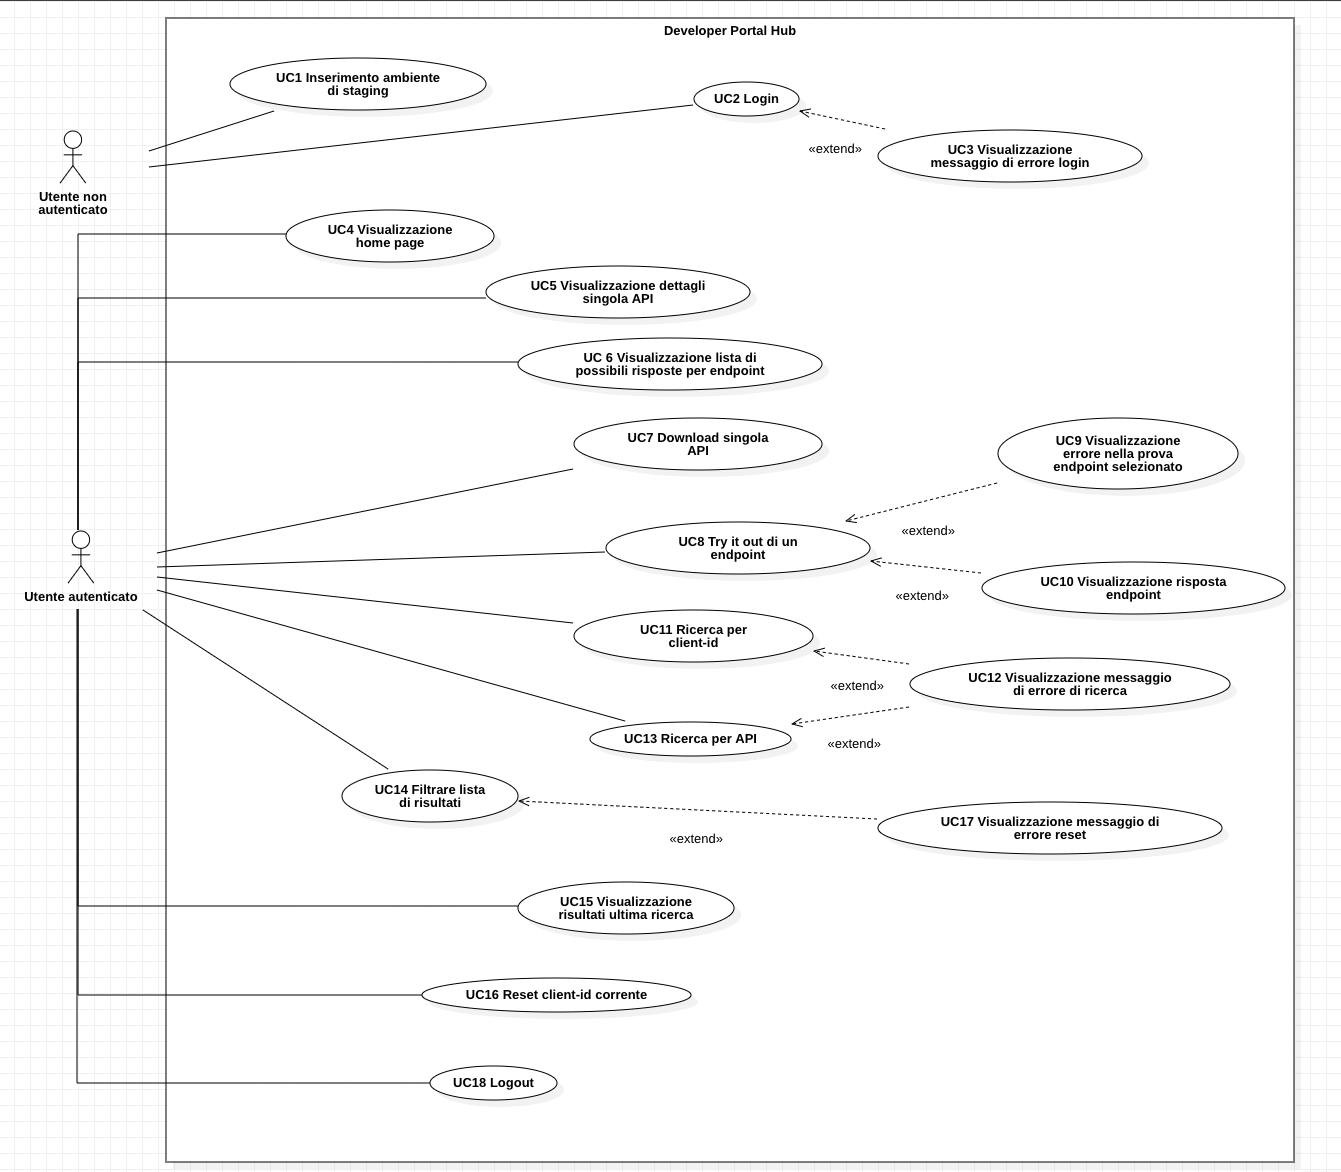
\includegraphics[width=0.85\columnwidth, alt={Scenario principale dei casi d'uso individuati}]{images/usecase/scenario-principale.jpg}
    \caption{Scenario principale}\label{fig:usecase-scenario-principale}
\end{figure}

\clearpage


% UC 1 - Inserimento ambiente di staging
\begin{usecase}{1}{Inserimento ambiente di staging}\label{uc:inserimento-ambiente-di-staging}
    \usecaseactors{Utente non autenticato}
    \usecasepre{L'utente non è autenticato e non ha ancora avviato l'applicazione web}
    \usecasedesc{L'utente vuole avviare l'applicazione web e deve scegliere in che ambiente di staging farlo}
    \usecasepost{L'utente avvia l'applicazione nell'ambiente di staging scelto}

    \usecasemain{}
        \begin{enumerate}
            \item L'utente seleziona il link del portale a seconda dell'ambiente di staging che vuole avviare (development, quality e production)
        \end{enumerate}

\end{usecase}

% UC 2 - Login
\begin{usecase}{2}{Login}\label{uc:login}
    \usecaseactors{Utente non autenticato, Microsoft 365}
    \usecasepre{ L'utente possiede un account valido per autenticazione tramite Microsoft 365 che appartiene al gruppo autorizzato per il login al sistema. Inoltre l'utente non è autenticato e si trova nella pagina di login}
    \usecasedesc{L'utente vuole accedere al sistema e deve inserire le proprie credenziali per accedervi}
    \usecasepost{L'utente è autenticato correttamente e può procedere con l'utilizzo di tutte le funzionalità disponibili all'interno del sistema}

    \usecasemain{}
        \begin{enumerate}
            \item L'utente inserisce la propria e-mail;
            \item L'utente inserisce la propria password;
            \item Microsoft 365 verifica le credenziali inserite, in base ai permessi configurati.
        \end{enumerate}

    \usecaseext{}
    \begin{enumerate}
        \item Visualizzazione messaggio di errore login UC3.
    \end{enumerate}

    \usecasegen{}
    \begin{enumerate}
        \item Inserimento e-mail UC2.1;
        \item Inserimento password UC2.2.
    \end{enumerate}

\end{usecase}

\begin{figure}[!ht] 
    \centering 
    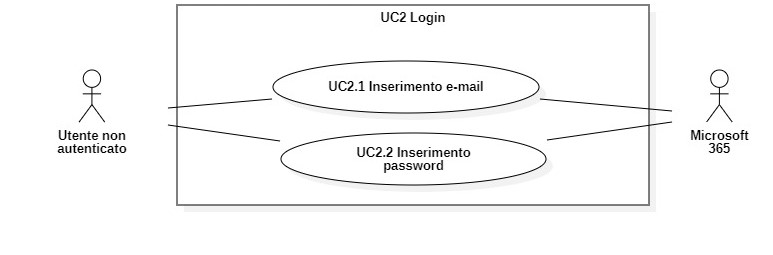
\includegraphics[width=0.9\columnwidth, alt={Caso d'uso relativo al login}]{images/usecase/UC2.jpg}
    \caption{UC2 Login}\label{fig:uc:login}
  \end{figure}
  
%   \newpage


% UC 2.1 - Inserimento e-mail
\begin{usecase}{2.1}{Inserimento e-mail}\label{uc:inserimento-email}
    \usecaseactors{Utente non autenticato}
    \usecasepre{L'utente possiede un account valido per autenticazione tramite Microsoft 365 che appartiene al gruppo autorizzato per il login al sistema. Inoltre l'utente non è autenticato e si trova nella pagina di login}
    \usecasedesc{L'utente deve inserire la propria e-mail per autenticarsi al sistema}
    \usecasepost{L'utente ha inserito la propria e-mail, può quindi procedere a completare il processo di autenticazione}

    \usecasemain{}
        \begin{enumerate}
            \item L'utente inserisce nell'apposito campo la propria e-mail.
        \end{enumerate}

\end{usecase}


% UC 2.2 - Inserimento password
\begin{usecase}{2.2}{Inserimento password}\label{uc:inserimento-password}
    \usecaseactors{Utente non autenticato}
    \usecasepre{L'utente possiede un account valido per autenticazione tramite Microsoft 365 che appartiene al gruppo autorizzato per il login al sistema. Inoltre l'utente non è autenticato e si trova nella pagina di login}
    \usecasedesc{L'utente deve inserire la propria password per autenticarsi al sistema}
    \usecasepost{L'utente ha inserito la propria password e può concludere il processo di autenticazione}

    \usecasemain{}
        \begin{enumerate}
            \item L'utente inserisce nell'apposito campo la propria password.
        \end{enumerate}

\end{usecase}

\clearpage
% UC 3 - Visualizzazione messggio di errore login
\begin{usecase}{3}{Visualizzazione messggio di errore login}\label{uc:visualizzazione-errore-login}
    \usecaseactors{Utente non autenticato}
    \usecasepre{L'utente ha inserito una tra le due credenziali email o password in modo errato}
    \usecasedesc{L'utente deve inserire delle credenziali corrette per poter effettuare il login correttamente}
    \usecasepost{L'utente ha inserito una tra le due credenziali errate}

    \usecasemain{}
        \begin{enumerate}
            \item L'utente visualizza un messaggio di errore che lo informa che una delle credenziali che ha inserito per autenticarsi al sistema è sbagliata.
        \end{enumerate}

\end{usecase}


% UC 4 - Visualizzazione home page
\begin{usecase}{4}{Visualizzazione home page}\label{uc:visualizzasioen-home-page}
    \usecaseactors{Utente autenticato}
    \usecasepre{L'utente è autenticato ed è stato reindirizzato alla pagina principale}
    \usecasedesc{L'utente vuole visualizzare la pagina principale}
    \usecasepost{L'utente ha visualizzato la pagina principale}

    \usecasemain{}
        \begin{enumerate}
            \item L'utente visualizza la pagina principale.
        \end{enumerate}

    \usecasegen{}
        \begin{enumerate}
            \item Visualizzazione lista APIs disponibili UC4.1;
            \item Visualizzazione client-id di default UC4.2;
            \item Visualizzazione dettagli utente autenticato UC4.3.
        \end{enumerate}

\end{usecase}

\begin{figure}[!ht] 
    \centering 
    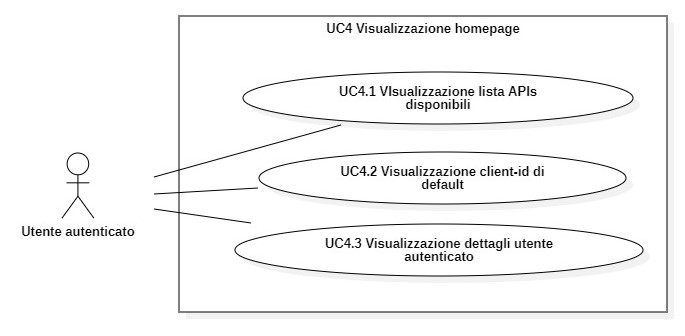
\includegraphics[width=0.9\columnwidth, alt={Caso d'uso relativo alla visualizzazione della homepage}]{images/usecase/UC4.jpg}
    \caption{UC4 Visualizzazione home page}\label{fig:uc:visualizzazione-home-page}
  \end{figure}

  \pagebreak


% UC 4.1 - Visualizzazione lista APIs disponibili
\begin{usecase}{4.1}{Visualizzazione lista APIs disponibili}\label{uc:visualizzazione-lista-apis-disponibili}
    \usecaseactors{Utente autenticato}
    \usecasepre{L'utente è autenticato ed è stato reindirizzato alla pagina principale}
    \usecasedesc{L'utente vuole visualizzare la lista di API disponibili per la consultazione all'interno del sistema}
    \usecasepost{L'utente ha visualizzato la lista di API disponibili all'interno del sistema}
    \usecasemain{}
        \begin{enumerate}
            \item L'utente visualizza la lista di API disponibili all'interno del sistema.
        \end{enumerate}

\end{usecase}

% UC 4.2 - Visualizzazione client-id di default
\begin{usecase}{4.2}{Visualizzazione client-id di default}\label{uc:visualizzazione-client-id-di-default}
    \usecaseactors{Utente autenticato}
    \usecasepre{L'utente è autenticato ed è stato reindirizzato alla pagina principale}
    \usecasedesc{L'utente vuole visualizzare il client-id di default impostato nell'ambiente corrente}
    \usecasepost{L'utente ha visualizzato il client-id di default impostato nell'ambiente corrente in cui si trova}

    \usecasemain{}
        \begin{enumerate}
            \item L'utente visualizza il client-id di default impostato nell'ambiente corrente in cui si trova.
        \end{enumerate}

\end{usecase}

\clearpage

% % UC 4.3 Visualizzazione dettagli utente autenticato
\begin{usecase}{4.3}{Visualizzazione dettagli utente autenticato}\label{uc:visualizzazione-dettagli-utente-autenticato}
    \usecaseactors{Utente autenticato}
    \usecasepre{L'utente è autenticato ed è stato reindirizzato alla pagina principale}
    \usecasedesc{L'utente vuole visualizzare i propri dati personali, ovvero del proprio utente autenticato}
    \usecasepost{L'utente visualizza i dati personali del proprio account autenticato nel sistema}

    \usecasemain{}
        \begin{enumerate}
            \item L'utente visualizza le informazioni personali del proprio account autenticato nel sistema.
        \end{enumerate}

\end{usecase}

% UC 5 Visualizzazione dettagli singola API
\begin{usecase}{5}{Visualizzazione dettagli singola API}\label{uc:visualizzazione-dettagli-singola-api}
    \usecaseactors{Utente autenticato}
    \usecasepre{L'utente è autenticato e si trova nella pagina principale}
    \usecasedesc{L'utente vuole visualizzare la pagina di dettaglio di una singola API}
    \usecasepost{L'utente ha visualizzato la pagina di dettaglio di una singola API tra quelle presenti nel sistema}

    \usecasemain{}
        \begin{enumerate}
            \item L'utente clicca su una delle API presenti nella lista di API disponibili all'interno del sistema.
            \item L'utente visualizza la pagina di dettaglio della singola API selezionata.
        \end{enumerate}

    \usecasegen{}
        \begin{enumerate}
            \item Visualizzazione lista endpoint disponibili UC5.1.
        \end{enumerate}

\end{usecase}

\begin{figure}[!ht] 
    \centering 
    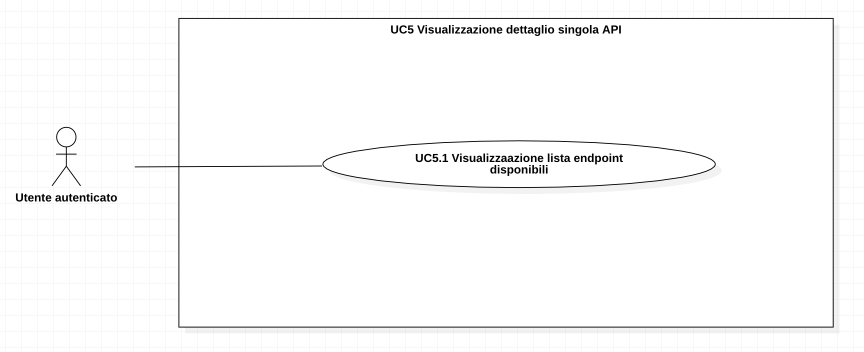
\includegraphics[width=0.9\columnwidth, alt={Caso d'uso relativo alla visualizzazione del dettaglio di una singola API}]{images/usecase/UC5.jpg}
    \caption{UC5 Visualizzazione dettaglio singola API}\label{fig:uc:visualizzazione-dettaglio-singola-api}
  \end{figure}

  \pagebreak

% UC 5.1 Visualizzazione lista endpoint disponibili
\begin{usecase}{5.1}{Visualizzazione lista endpoint disponibili}\label{uc:visualizzazione-lista-endpoint-disponibili}
    \usecaseactors{Utente autenticato}
    \usecasepre{L'utente è autenticato e sta visualizzando la pagina di dettaglio di una singola API}
    \usecasedesc{L'utente vuole visualizzare la lista completa di endpoint disponibili per l'API}
    \usecasepost{L'utente visualizza la lista completa di endpoint disponibili per l'API}

    \usecasemain{}
        \begin{enumerate}
            \item L'utente visualizza la lista completa di endpoint disponibili per l'API che ha selezionato.
        \end{enumerate}

    \usecasegen{}
        \begin{enumerate}
            \item Visualizzazione dettaglio singolo endpoint UC5.1.1.
        \end{enumerate}

\end{usecase}

\begin{figure}[!ht] 
    \centering 
    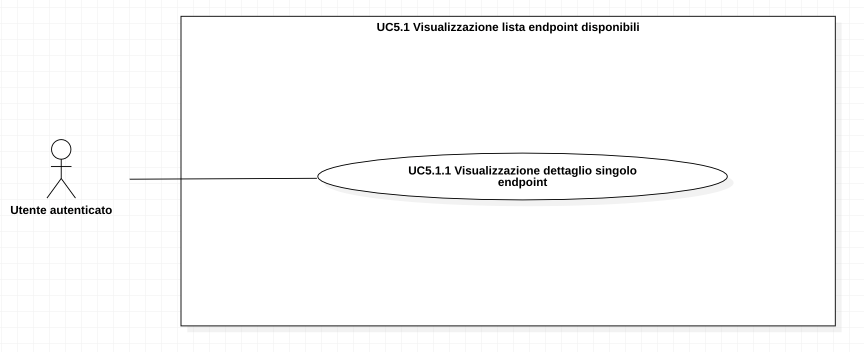
\includegraphics[width=0.9\columnwidth, alt={Caso d'uso relativo al visualizzazione della lista di endpoint disponibili}]{images/usecase/UC5.1.jpg}
    \caption{UC5.1 Visualizzazione lista endpoint disponibili}\label{fig:uc:visualizzazione-lista-endpoint-disponibili}
  \end{figure}
  \pagebreak


% UC 5.1.1 Visualizzazione dettaglio singolo endpoint
\begin{usecase}{5.1.1}{Visualizzazione dettaglio singolo endpoint}\label{uc:visualizzazione-dettaglio-singolo-endpoint}
    \usecaseactors{Utente autenticato}
    \usecasepre{L'utente è autenticato, sta visualizzando la pagina di dettaglio di una singola API contenente la lista di endpoint disponibili}
    \usecasedesc{L'utente vuole visualizzare la pagina di dettaglio di un singolo endpoint}
    \usecasepost{L'utente visualizza la pagina di dettaglio di un singolo endpoint}

    \usecasemain{}
        \begin{enumerate}
            \item L'utente clicca sullo specifico endpoint che vuole visualizzare;
            \item L'utente visualizza i dettagli disponibili per l'endpoint selezionato.
        \end{enumerate}

    \usecaseext{}
        \begin{enumerate}
            \item Visualizzazione lista di possibili risposte endpoint UC6.
        \end{enumerate}

\end{usecase}


% UC 6 Visualizzazione lista di possibili risposte endpoint
\begin{usecase}{6}{Visualizzazione lista di possibili risposte endpoint}\label{uc:visualizzazione-risposte-endpoint}
    \usecaseactors{Utente autenticato}
    \usecasepre{L'utente è autenticato, sta visualizzando la sezione di dettaglio di un singolo endpoint}
    \usecasedesc{L'utente vuole visualizzare la lista dei possibili risultati possibili per l'endpoint selezionato}
    \usecasepost{L'utente visualizza la lista delle possibili risposte disponibili per l'endpoint che ha selezionato}

    \usecasemain{}
        \begin{enumerate}
            \item L'utente visualizza i dettagli riguardanti le possibili risposte che l'endpoint selezionato può ritornare.
        \end{enumerate}

\end{usecase}


% UC 7 Download singola API
\begin{usecase}{7}{Download singola API}\label{uc:download-singola-api}
    \usecaseactors{Utente autenticato}
    \usecasepre{L'utente è autenticato ed ha selezionato una API dalla lista di API disponibili nel sistema}
    \usecasedesc{L'utente vuole poter scaricare in formato YAML un API dal portale}
    \usecasepost{L'utente ha scaricato in formato YAML un API dal portale}

    \usecasemain{}
        \begin{enumerate}
            \item L'utente scarica il formato YAML di un API dal portale, tra quelle disponibili;
            \item Una nuova pagina si apre e il download dell'API viene eseguito;
            \item Il nome del file è già impostato con il nome dell'API scaricata.
        \end{enumerate}

\end{usecase}


% UC 8 Try it out endpoint
\begin{usecase}{8}{Try it out endpoint}\label{uc:try-it-out-endpoint}
    \usecaseactors{Utente autenticato}
    \usecasepre{L'utente è autenticato, sta visualizzando i dettagli di un singolo endpoint di un API disponibile nel sistema}
    \usecasedesc{L'utente vuole poter provare l'endpoint selezionato}
    \usecasepost{L'utente ha provato l'endpoint selezionato}

    \usecasemain{}
        \begin{enumerate}
            \item L'utente ha selezionato una determinata API;
            \item L'utente ha selezionato un determinato endpoint di quell'API;
            \item L'utente ha cliccato sul pulsante per provare l'endpoint selezionato.
        \end{enumerate}

    \usecaseext{}
        \begin{enumerate}
            \item Visualizzazione errore nella prova dell'endpoint selezionato UC9;
            \item Visualizzazione risposta endpoint UC10.
        \end{enumerate}

    \usecasegen{}
        \begin{enumerate}
            \item Inserimento parametri per try it out endpoint UC8.1;
            \item Definire campi aggiuntivi per try it out endpoint UC8.2.
        \end{enumerate}

\end{usecase}

\begin{figure}[!ht] 
    \centering 
    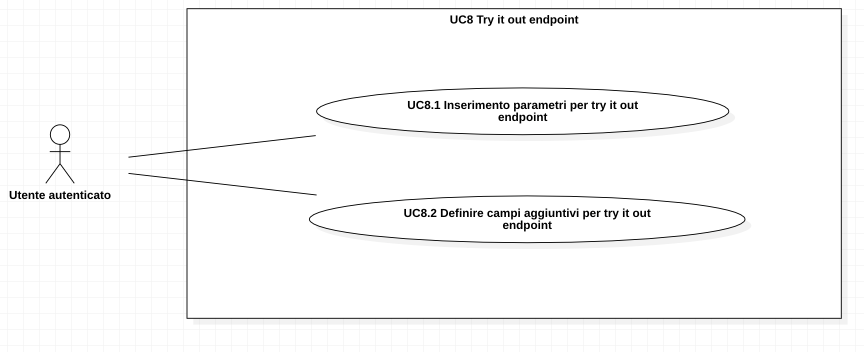
\includegraphics[width=0.9\columnwidth, alt={Caso d'uso relativo alla prova di un endpoint}]{images/usecase/UC8.jpg}
    \caption{UC8 Try it out endpoint}\label{fig:uc:try-it-out-endpoint}
\end{figure}

\\

% UC 8.1 Inserimento parametri necessari per la prova dell'endpoint     
\begin{usecase}{8.1}{Inserimento parametri per try it out endpoint}\label{uc:inserimento-parametri-try-it-out-endpoint}
    \usecaseactors{Utente autenticato}
    \usecasepre{L'utente è autenticato, sta visualizzando la schermata di try it out nella sezione di inserimento dei parametri}
    \usecasedesc{L'utente vuole poter inserire i parametri necessari per la prova dell'endpoint}
    \usecasepost{L'utente ha inserito i parametri necessari alla chiamata verso l'endpoint}

    \usecasemain{}
        \begin{enumerate}
            \item L'utente inserisce i parametri richiesti per la chiamata verso l'endpoint selezionato.
        \end{enumerate}

\end{usecase}


% UC 8.2 Definire campi aggiuntivi per try it out endpoint
\begin{usecase}{8.2}{Definire campi aggiuntivi per try it out endpoint}\label{uc:definire-campi-try-it-out-endpoint}
    \usecaseactors{Utente autenticato}
    \usecasepre{L'utente è autenticato, sta visualizzando la schermata di try it out nella sezione dei parametri aggiuntivi}
    \usecasedesc{L'utente vuole poter definire dei campi aggiuntivi ai parametri già esistenti, per poi andare a provare la chiamata verso l'endpoint}
    \usecasepost{L'utente ha creato dei parametri aggiuntivi per la chiamata verso l'endpoint}

    \usecasemain{}
        \begin{enumerate}
            \item L'utente definisce dei parametri da aggiungere a quelli già esistenti.
        \end{enumerate}

\end{usecase}

% UC 9 Visualizzazione errore nella prova dell'endpoint selezionato
\begin{usecase}{9}{Visualizzazione errore nella prova dell'endpoint selezionato}\label{uc:visualizzazione-errore-prova-endpoint-selezionato}
    \usecaseactors{Utente autenticato}
    \usecasepre{L'utente è autenticato, è nella sezione di prova di un endpoint ed ha inserito dei parametri errati}
    \usecasedesc{L'utente deve inserire dei parametri corretti per poter provare l'endpoint senza riscontrare errori} 
    \usecasepost{L'utente ha inserito dei parametri parzialmente o in modo scorretto e non può procedere con l'esecuzione della chiamata}

    \usecasemain{}
        \begin{enumerate}
            \item L'utente visualizza un messaggio di errore che lo avvisa che i parametri inseriti non sono corretti, o risultano incompleti.
        \end{enumerate}

\end{usecase}


% UC 10 Visualizzazione risposta endpoint
\begin{usecase}{10}{Visualizzazione risposta endpoint}\label{uc:visualizzazione-risposta-endpoint}
    \usecaseactors{Utente autenticato}
    \usecasepre{L'utente è autenticato, è nella sezione di prova di un endpoint ed ha inserito dei parametri corretti}
    \usecasedesc{L'utente vuole visualizzare la risposta dell'endpoint}
    \usecasepost{L'utente visualizza la risposta adeguata alla chiamata verso l'endpoint, in base ai parametri inseriti}

    \usecasemain{}
        \begin{enumerate}
            \item L'utente visualizza la risposta dell'endpoint, uno tra quelle possibili contenute nella descrizione dell'endpoint. La risposta varia in base ai parametri inseriti.
        \end{enumerate}

\end{usecase}

\clearpage

% UC 11 Ricerca per client-id
\begin{usecase}{11}{Ricerca per client-id}\label{uc:ricerca-client-id}
    \usecaseactors{Utente autenticato}
    \usecasepre{L'utente è autenticato e sta navigando all'interno del sistema} 
    \usecasedesc{L'utente vuole poter ricercare un client-id all'interno del sistema}
    \usecasepost{L'utente effettua una ricerca per client-id e il sistema ha restituito i risultati della ricerca}

    \usecasemain{}
        \begin{enumerate}
            \item L'utente clicca il bottone per effettuare la ricerca per client-id;
            \item L'utente inserisce nell'apposito campo il client-id che vuole cercare all'interno del sistema;
            \item Il sistema ricerca il client-id inserito e restituisce i risultati della ricerca;
            \item Il sistema aggiunge l'ultima ricerca effettuata alla cronologia delle ultime ricerche.
        \end{enumerate}

    \usecaseext{}
        \begin{enumerate}
            \item Visualizzazione messaggio di errore di ricerca UC 12.
        \end{enumerate}

\end{usecase}


% % UC 12 Visualizzazione messaggio di errore di ricerca
\begin{usecase}{12}{Visualizzazione messaggio di errore di ricerca}\label{uc:visualizzazione-errore-ricerca}
    \usecaseactors{Utente autenticato}
    \usecasepre{L'utente è autenticato e ha cercato un client-id o un API inesistente nel sistema}
    \usecasedesc{L'utente deve inserire un client-id o un API esistente nel sistema per poter effettuare la ricerca. Inoltre il client-id deve esistere per l'ambiente selezionato}
    \usecasepost{L'utente ha inserito un client-id o un API inesistente nel sistema e visualizza un messaggio di errore}

    \usecasemain{}
        \begin{enumerate}
            \item L'utente visualizza un messaggio di errore che lo informa che la ricerca effettuata non ha prodotto nessun risultato, indicando che ciò è dovuto al fatto
            che il client-id o l'API cercata non è presente nel sistema, oppure non esiste quel client-id per l'ambiente selezionato.
        \end{enumerate}

\end{usecase}

\clearpage
% UC 13 Ricerca per API
\begin{usecase}{13}{Ricerca per API}\label{uc:ricerca-api}
    \usecaseactors{Utente autenticato}
    \usecasepre{L'utente è autenticato e sta navigando all'interno del sistema}
    \usecasedesc{L'utente vuole poter ricercare un API all'interno del sistema}
    \usecasepost{L'utente effettua una ricerca per API e il sistema ha restituito i risultati della ricerca}

    \usecasemain{}
        \begin{enumerate}
            \item L'utente clicca il bottone per effettuare la ricerca per API;
            \item L'utente inserisce nell'apposito campo l'API che vuole cercare all'interno del sistema;
            \item Il sistema ricerca l'API inserita e restituisce i risultati della ricerca;
            \item Il sistema aggiunge l'ultima ricerca effettuata alla cronologia delle ultime ricerche.
        \end{enumerate}

    \usecaseext{}
        \begin{enumerate}
            \item Visualizzazione messaggio di errore di ricerca UC12.
        \end{enumerate}

\end{usecase}


% UC 14 Reset client-id corrente
\begin{usecase}{14}{Reset client-id corrente}\label{uc:reset-client-id}
    \usecaseactors{Utente autenticato}
    \usecasepre{L'utente è autenticato, sta navigando all'interno del sistema e ha già selezionato un client-id che non è quello di default} 
    \usecasedesc{L'utente vuole poter resettare il client-id corrente e tornare al client-id di default per l'ambiente selezionato}
    \usecasepost{L'utente ha resettato il client-id corrente e ora visualizza il client-id di default per l'ambiente selezionato}

    \usecasemain{}
        \begin{enumerate}
            \item L'utente clicca il bottone per resettare il client-id corrente;
            \item Il sistema resetta il client-id corrente ed imposta il client-id al valore di default a seconda dell'ambiente selezionato.
        \end{enumerate}

        \clearpage
    \usecaseext{}
        \begin{enumerate}
            \item Visualizzazione messaggio di errore reset UC15.
        \end{enumerate}

\end{usecase}


% UC 15 Visualizzazione messaggio di errore reset
\begin{usecase}{15}{Visualizzazione messaggio di errore reset}\label{uc:visualizzazione-errore-reset}
    \usecaseactors{Utente autenticato}
    \usecasepre{L'utente è autenticato e ha provato a resettare il client-id corrente che è quello di default per l'ambiente selezionato}
    \usecasedesc{L'utente deve aver selezionato un client-id diverso da quello di default, per poterlo resettare}
    \usecasepost{L'utente ha provato a resettare il client-id corrente, ma risulta essere quello di default}

    \usecasemain{}
        \begin{enumerate}
            \item L'utente visualizza un messaggio di errore che lo informa che il client-id corrente è quello di default per l'ambiente selezionato e non può essere resettato.
        \end{enumerate}

\end{usecase}


% UC 16 Logout
\begin{usecase}{16}{Logout}\label{uc:}
    \usecaseactors{Utente autenticato, Microsoft 365}
    \usecasepre{L'utente è autenticato e vuole uscire dalla sessione corrente}
    \usecasedesc{L'utente vuole effettuare il logout dal sistema}
    \usecasepost{L'utente effettua il logout dal sistema terminando la sessione corrente, non è più autenticato e viene reindirizzato alla pagina di login}

    \usecasemain{}
        \begin{enumerate}
            \item L'utente clicca il bottone per effettuare il logout;
            \item Microsoft 365 effettua il logout dell'utente terminando la sessione.
        \end{enumerate}

\end{usecase}

\clearpage

\section{Tracciamento dei requisiti}

In questa sezione vengono riportati i requisiti indiduati durante il progetto di stage.
Questo capitolo si sofferma in particolare sulla classificazione dei requisiti in tre categorie principali:
\begin{itemize}
    \item \textbf{Requisiti funzionali}: delineano le funzionalità che il sistema deve offrire. Essi delineano le azioni specifiche che il sistema deve eseguire, le risposte attese a determinati input e le dinamiche generali delle operazioni;
    \item\textbf{Requisiti qualitativi}: definiscono gli aspetti legati alla qualità, all'usabilità e alle prestazioni del sistema;
    \item \textbf{Requisiti di vincolo}: delineano le restrizioni e i parametri che il sistema deve rispettare durante lo sviluppo e l'implementazione. 
\end{itemize}

Inoltre viene fatta una classificazione dei requisiti in base alla priorità assegnata a ciascun requisito.

\subsubsection{Notazione}
Ciascun requisito è identificato da un codice univoco, che segue la seguente notazione:
\begin{center}
    \textbf{R[Priorità][Tipo]-[Codice]}
\end{center}
  dove:
  \begin{itemize}
  \item \textbf{Priorità} indica il livello di priorità assegnato: obbligatorio (\textbf{O}), desiderabile (\textbf{D}) e opzionale (\textbf{Z}) ;
  \item \textbf{Tipo} indica il tipo di requisito: funzionale (\textbf{F}) , qualititativo (\textbf{Q}) e di vincolo (\textbf{V});
  \item \textbf{Codice} indica il codice identificativo del requisito.
  \end{itemize}

Nelle tabelle \ref{tab:requisiti-funzionali}, \ref{tab:requisiti-qualitativi} e \ref{tab:requisiti-vincolo} sono riassunti i requisiti tramite una breve descrizione accompagnata dalle fonti da cui è stato individuato il requisito per
facilitarne la tracciabilità. 

% \newpage

\subsubsection{Requisiti funzionali}

% \renewcommand{\arraystretch}{1.1} % Adjust the spacing inside the cells
% % Redefine column type to center the content
% \newcolumntype{C}[1]{>{\arraybackslash}p{#1}}

\begin{center}
\captionof{table}{Tabella del tracciamento dei requisiti funzionali}\label{tab:requisiti-funzionali}
\begin{longtable}{|c|p{0.6\textwidth}|c|}
\hline
\textbf{Requisito} & \textbf{Descrizione} & \textbf{Fonte}\\
\hline
RFO-1 &L'utente deve scegliere l'ambiente di staging & UC1 \\
\hline
RFO-2 &Il sistema deve permettere l'autenticazione ad un utente con un account valido & UC2 \\
\hline
RFO-2.1 & L'utente deve inserire la propria mail & UC2.1 \\
\hline
% \textit{username}
RFO-2.2 & L'utente deve inserire la propria password & UC2.2 \\
\hline
RFO-3 &Il sistema deve avvisare l'utente tramite un messaggio di errore che le credenziali inserite nel login sono errate & UC3 \\
\hline
RFO-4 &Il sistema deve reindirizzare l'utente alla pagina principale, dopo che il login è andato a buon fine & UC4 \\
\hline
RFO-4.1 &L'utente deve poter visualizzare la lista di API disponibili nel sistema & UC4.1 \\
\hline
RFO-4.2 &L'utente deve poter visualizzare la lista di client-id di default impostata nell'ambiente di staging in cui si trova & UC4.2 \\
\hline
RFO-4.3 &L'utente deve poter visualizzare i dettagli relativi al suo account & UC4.3 \\
\hline
RFO-5 &L'utente deve poter visualizzare i dettagli relativi ad una singola API  & UC5 \\
\hline
RFO-5.1 &L'utente deve poter visualizzare la lista di endpoint disponibili all'interno del sistema & UC5.1 \\
\hline
RFO-5.1.1 &L'utente deve poter visualizzare i dettagli relativi ad un singolo endpoint di una determinata API & UC5.1.1 \\
\hline
RFO-6 &L'utente deve poter visualizzare l'elenco delle possibili risposte per il determinato endpoint selezionato & UC6 \\
\hline
RFO-7 &Il sistema deve permettere il download all'utente di una singola API & UC7 \\
\hline
RFO-8 &Il sistema deve permettere il try it out di un singolo endpoint all'utente & UC8 \\
\hline
RFO-8.1 &Il sistema deve permettere l'inserimento dei parametri necessari per il try it out di un endpoint & UC8.1 \\
\hline
RFD-8.2 &Il sistema deve permettere la possibilità di definire dei campi aggiuntivi per il try it out di un endpoint & UC8.2 \\
\hline
RFO-9 &Il sistema deve avvisare l'utente tramite un messaggio di errore che i parametri inseriti non sono corretti o incompleti & UC9 \\
\hline
RFO-10 &L'utente deve poter visualizzare la risposta dell'endpoint che ha provato & UC10 \\
\hline
RFO-11 &Il sistema deve permettere all'utente di poter effettuare una ricerca per client-id & UC11 \\
\hline
RFO-12 &Il sistema deve avvisare l'utente tramite un messaggio di errore che la ricerca effettuata non ha portato a risultati presenti nel sistema & UC12 \\
\hline
RFO-13 &Il sistema deve permettere all'utente di poter effettuare una ricerca per API & UC13 \\
\hline
RFD-14 &Il sistema deve permettere il reset del client-id corrente & UC14 \\
\hline
RFO-15 &Il sistema deve avvisare l'utente tramite un messaggio di errore che il client-id è già di default & UC15 \\
\hline
RFO-16 &Il sistema deve permettere il logout all'utente, uscendo dalla sessione  & UC16 \\
\hline
\end{longtable}
\end{center}

\subsubsection{Requisiti qualitativi}

% \renewcommand{\arraystretch}{1.1} 
% \newcolumntype{C}[1]{>{\arraybackslash}p{#1}}

\begin{center}
\captionof{table}{Tabella del tracciamento dei requisiti qualitativi}\label{tab:requisiti-qualitativi}
\begin{longtable}{|c|p{0.6\textwidth}|c|}
\hline
\textbf{Requisito} & \textbf{Descrizione} & \textbf{Fonte}\\
\hline
RQO-1 &Il progetto deve essere accompagnato da documentazione tecnica e funzionale & Interno \\
\hline
RQO-2 &La parte frontend del progetto deve essere coperta da test di unità & Interno \\
\hline
RQZ-3 &L'applicazione web deve avere un'interfaccia responsive & Interno \\
\hline
RQD-5 &L'applicativo deve essere accessibile utilizzando i principali browser & Interno \\
\hline
\end{longtable}
\end{center}


\subsubsection{Requisiti di vincolo}

% \renewcommand{\arraystretch}{1.1} 
% \newcolumntype{C}[1]{>{\arraybackslash}p{#1}}

\begin{center}
\captionof{table}{Tabella del tracciamento dei requisiti di vincolo}\label{tab:requisiti-vincolo}
\begin{longtable}{|c|p{0.6\textwidth}|c|}
\hline
\textbf{Requisito} & \textbf{Descrizione} & \textbf{Fonte}\\
\hline
RVO-1 & L'applicazione deve essere sviluppata utilizzando il framework Vue.js 3, usando Typescript come linguaggio di programmazione & UC1 \\
\hline
RVO-2 & I componenti devono essere scritti utilizzando le Composition API di Vue.js 3 & UC1 \\
\hline
RVD-3 & I componenti di base devono essere implementati utilizzando la libreria THRON Components & UC2 \\
\hline
RVZ-4 & L'interfaccia dell'applicazione deve seguire il design system THRON & UC2 \\
\hline
\end{longtable}
\end{center}
    \chapter{Struttura principale e progettazione}\label{cap:struttura-progettazione}

\intro{In questo capitolo sono descritte la struttura principale del progetto e le attività di progettazione dell'applicativo.
Inoltre vengono descritte le tecnologie utilizzate durante lo sviluppo del progetto e le scelte architetturali.
}

\section{Tecnologie utilizzate}\label{sec:tecnologie-utilizzate}
Di seguito viene data una panoramica delle tecnologie utilizzate durante lo sviluppo del progetto di stage.

\subsection{Frontend}\label{subsec:frontend}
\subsubsection{Vue.js}\label{subsubsec:vue-js}
\textit{Vue.js} è un \textit{framework JavaScript} progressivo e reattivo, utilizzato per lo sviluppo di interfacce utente dinamiche e moderne. 
Creato da \textit{Evan You}, \textit{Vue.js} è apprezzato per la sua semplicità d'uso e flessibilità. Con un sistema di reattività basato su un modello di oggetti e dipendenze, 
\textit{Vue.js} rende facile il monitoraggio e l'aggiornamento automatico dell'interfaccia utente in base ai cambiamenti di stato dei dati. La sua architettura basata 
su componenti consente di organizzare il codice in moduli riutilizzabili e autonomi, semplificando la creazione di applicazioni complesse. 
Grazie alle direttive, è possibile arricchire il \glsfirstoccur{\gls{domg}} con funzionalità reattive, mentre il sistema di \textit{routing} agevola la creazione di \glsfirstoccur{\gls{spag}}. 
Con una crescita costante della comunità di sviluppatori, \textit{Vue.js} è diventato un'opzione popolare nel mondo dello sviluppo frontend.
Per il mio progetto ho utilizzato la versione 3 di \textit{Vue.js}, insieme allo \textit{script setup}, che è una nuova sintassi per definire componenti, progettata per semplificare la struttura del codice~\cite{site:vue.js}.

\subsubsection{TypeScript}\label{subsubsec:typeScript}
\textit{TypeScript} è un linguaggio di programmazione \glsfirstoccur{\gls{opensourceg}} sviluppato da \textit{Microsoft}. Si basa su \textit{JavaScript} e offre tipizzazione statica opzionale, 
consentendo agli sviluppatori di specificare tipi per variabili, parametri di funzioni e oggetti. Questa caratteristica aiuta a individuare errori e a migliorare 
la manutenibilità del codice~\cite{site:typescript}.\\
All'interno del mio progetto ho creato per la parte frontend una cartella chiamata \textit{types}, che contiene un file \textit{TypeScript} con al suo interno tutti i tipi utilizzati nel progetto.
\subsubsection{Vite.js}\label{subsubsec:vite}
\textit{Vite.js} è un \textit{build tool} utilizzato per lo sviluppo di applicazioni web. È stato creato da \textit{Evan You}, lo stesso creatore di \textit{Vue.js}, e si basa su \glsfirstoccur{\gls{rollupjsg}}.
\textit{Vite.js} è stato progettato per essere veloce, semplice da utilizzare e facile da configurare. La sua velocità è dovuta al fatto che utilizza la tecnica dell'\glsfirstoccur{\gls{esmg}} (\textit{ECMAScript Modules})
che permette di caricare i moduli in modo asincrono, riducendo i tempi di compilazione e di \glsfirstoccur{\gls{hotreloadg}}~\cite{site:vite}.
\subsubsection{Sass}\label{subsubsec:sass}
\textit{Sass} è un'estensione di \textit{CSS} che offre funzionalità aggiuntive e avanzate per semplificare e organizzare il modo in cui viene scritto e gestito il codice.
Può essere considerato un preprocessore \textit{CSS}, in quanto viene compilato in \textit{CSS} prima di essere interpretato dal \textit{browser}. \textit{Sass} inoltre permette di utilizzare funzionalità non disponibili in \textit{CSS} nativo, offrendo una serie di funzioni, variabili, \glsfirstoccur{\gls{mixing}} e altro~\cite{site:sass}.\\
Insieme a \textit{Sass}, ho utilizzato \textit{BEM}, ovvero una metodologia di \textit{naming convention} utilizzata nel mondo dello sviluppo web.

\subsection{Backend}\label{subsec:backend}
\subsubsection{Nest.js}\label{subsubsec:nest-js}
\textit{Nest.js} è un \textit{framework} per applicazioni \textit{server-side} basato su \textit{Node.js}. Si basa su \glsfirstoccur{\gls{expressjsg}} e \textit{TypeScript} ed è progettato per creare applicazioni scalabili e performanti.
Il \textit{framework} in questione combina concetti e caratteristiche provenienti da diversi paradigmi di sviluppo, tra cui la programmazione orientata agli oggetti (OOP), la programmazione funzionale e la programmazione reattiva~\cite{site:nest.js}.

\subsection{Altre tecnologie di supporto}\label{subsec:altre-tecnologie-di-supporto}
\subsubsection{Node.js}\label{subsubsec:node-js}
\textit{Node.js} è un ambiente di \textit{runtime JavaScript open-source} progettato per eseguire codice lato server~\cite{site:node}. Per gestire le dipendenze del mio progetto,
ho deciso di utilizzare \glsfirstoccur{\gls{pnpmg}} come gestore di pacchetti. Questa selezione ha portato a un miglior utilizzo delle risorse di sistema e ha notevolmente accelerato il processo di 
installazione delle dipendenze.
\subsubsection{Pinia}\label{subsubsec:pinia}
\textit{Pinia} è una libreria per la gestione dello stato per applicazioni \textit{Vue.js}. Promuove l'uso di \textit{store} modulari, ognuno dei quali gestisce uno stato specifico dell'applicazione~\cite{site:pinia}.
\subsubsection{Vue-router}\label{subsubsec:vue-router}
\textit{Vue-router} è una libreria per la gestione delle \textit{route} per le applicazioni \textit{Vue.js}. Permette di definire le \textit{route} dell'applicazione e di navigare tra le pagine~\cite{site:vue-router}.

\subsection{Versionamento}\label{subsec:versionamento}
\subsubsection{Git}\label{subsubsec:git}
\textit{Git} è un sistema di controllo versione distribuito e altamente flessibile, utile per tenere traccia delle modifiche apportate al codice sorgente durante lo sviluppo di un progetto \glsfirstoccur{\gls{softwareg}}~\cite{site:git}.
\subsubsection{CodeCommit}\label{subsubsec:code-commit}
\textit{AWS CodeCommit} rappresenta un servizio di \textit{hosting} di \textit{repository} altamente scalabile, che è gestito all'interno dell'ecosistema di \glsfirstoccur{\gls{awsg}} (\textit{Amazon Web Services}). 
Con \textit{CodeCommit}, è possibile ospitare \textit{repository Git} privati in un ambiente sicuro e flessibile~\cite{site:code-commit}.

\subsection{Verifica}\label{subsec:verifica}
\subsubsection{ESLint}\label{subsubsec:eslint}
\textit{ESLint} è uno strumento \textit{open-source} ampiamente utilizzato per l'analisi statica del codice \textit{JavaScript}. Esso permette di identificare e segnalare potenziali errori o pratiche non conformi durante la fase di sviluppo.
\subsubsection{Vitest}\label{subsubsec:vitest}
\textit{Vitest} è un \textit{framework} per l'implementazione di test di unità, utilizzato prevalentemente in progetti \textit{Vue.js}.
Usato in coppia con \textit{Vite} permette di eseguire test di unità in modo più veloce e semplice~\cite{site:vitest}.

\subsection{Librerie esterne utilizzate}\label{subsec:librerie-esterne}
\subsubsection{THRON Components}\label{subsubsec:thron-components}
La libreria \textit{THRON Components} contiene i componenti utilizzati per creare elementi comuni, come i bottoni del portale, seguendo il \textit{design system} aziendale.
\subsubsection{Azure MSAL}\label{subsubsec:azure-MSAL}
\textit{Azure MSAL} è una libreria che permette di integrare il login con \glsfirstoccur{\gls{azureadg}} (\textit{Azure Active Directory}) all'interno di un'applicazione web~\cite{site:msal}.
\subsubsection{Swagger UI}\label{subsubsec:swagger-ui}
\textit{Swagger UI} è una libreria \textit{open-source} progettata per semplificare la visualizzazione e l'interazione con la documentazione delle \textit{API}~\cite{site:swagger}.

\section{Struttura principale del sistema}\label{sec:struttura-principale-sistema}
Il sistema è composto da due principali sezioni:
\begin{itemize}
  \item Frontend, ovvero l'interfaccia utente dell'applicazione web che permette all'utilizzatore di interagire con il sistema. È responsabile di presentare i contenuti in modo visivamente attraente e interattivo, consentendo agli utenti di navigare, inserire dati e svolgere azioni specifiche. Per lo
  sviluppo di questa parte del sistema è stato utilizzato il \textit{framework Vue.js};
  \item Backend, ovvero la parte del sistema che elabora le richieste provenienti dal frontend e restituisce i risultati. È responsabile della gestione dei dati e della logica di \textit{business}.
  Lo sviluppo di questa parte del sistema è stato realizzato utilizzando il \textit{framework Nest.js}. 
\end{itemize}

\subsection{Ambienti di sviluppo}\label{subsec:ambienti-sviluppo}
Gli ambienti di \textit{staging} sono ambienti di test che vengono utilizzati per testare le funzionalità dell'applicazione prima di rilasciarla in produzione.
A livello aziendale sono stati definiti tre ambienti di cui i primi due di \textit{staging}, denominati come segue:
\begin{itemize}
  \item \textbf{\textit{Development}}: consente di validare a livello tecnico le funzionalità;
  \item \textbf{\textit{Quality}}: consente di validare a livello funzionale o di implementazione le funzionalità;
  \item \textbf{\textit{Production}}: ambiente di produzione in cui viene rilasciata la funzionalità.
\end{itemize}

\subsection{Configurazione dell'ambiente per lo sviluppo del progetto}\label{subsec:configurazione-ambiente-sviluppo}
Il progetto di stage, necessita di cartelle per la configurazione dell'ambiente di sviluppo, per la configurazione del progetto e per la configurazione del \textit{deploy}.
Più precisamente, il progetto segue la seguente struttura:

\subsubsection*{\emph{Buildspec}}\label{subsubsec:buildspec}
La cartella \textit{Buildspec} contiene i file di configurazione per la \textit{build} dell'applicazione su \glsfirstoccur{\gls{awscodebuildg}}.
Questo è il primo step del processo di \textit{deploy}, in quanto viene eseguita la \textit{build} sia del \textit{middleware} che del portale.
La cartella è formata a sua volta da tre file: \textit{buildspec\_development}, \textit{buildspec\_quality} e \textit{buildspec\_production}. 
Ognuno di questi file configura la \textit{build} dell'applicazione in base all'ambiente di \textit{deploy}.\\
Successivamente dopo aver effettuato tutti i comandi specificati nei file \textit{buildspec}, inizia lo step di \textit{deploy}, specificato nella cartella \textit{Infra}.
Ognuno dei file \textit{buildspec} è un file \textit{YAML}, che è formato dalle seguenti sezioni:
\begin{itemize}
  \item La sezione \textit{env} dove vengono specificate le variabili d'ambiente utilizzate nel progetto;
  \item La sezione di \textit{pre-build} dove vengono specificati i comandi da eseguire prima della \textit{build};
  \item La sezione di \textit{build} dove vengono specificati i comandi per la \textit{build} del portale e del \textit{middleware}.
\end{itemize}

\subsubsection*{\emph{Infra}}\label{subsubsec:infra}
La cartella \textit{Infra} contiene i file di configurazione per il \textit{deploy} dell'applicazione su \textit{AWS}. È scritta utilizzando il linguaggio di programmazione \glsfirstoccur{\gls{pythong}}.\\
La cartella è formata da due file: `\textit{app.py}' e `\textit{stack.py}'. Il primo file contiene la configurazione per il \textit{deploy} dell'applicazione, mentre il secondo file contiene la configurazione per il \textit{deploy} dell'infrastruttura.\\
Per quanto riguarda l'infrastruttura del progetto, ho utilizzato e configurato due costrutti, anche chiamati \textit{CDK Constructs} o semplicemente \textit{Constructs}, che sono delle classi che rappresentano un componente dell'infrastruttura.
Il primo costrutto si chiama \textit{THRONCloudFrontDistribution} e consente di accelerare la distribuzione dei contenuti web statici e dinamici, come file \textit{HTML}, \textit{CSS}, \textit{JS} e immagini, agli utenti.
In breve questo costrutto genera il \textit{template} di \glsfirstoccur{\gls{awscloudfrontg}} ed esegue il \textit{deploy} degli \textit{asset} statici su un \glsfirstoccur{\gls{s3g}}.\\
Il secondo costrutto che ho utilizzato si chiama \textit{THRONDockerLambda} e consente di creare una funzione \glsfirstoccur{\gls{lambdag}} in cui il gestore è un'immagine \glsfirstoccur{\gls{dockerg}}.
Nel caso del mio progetto, mi è servito per creare una \textit{lambda} che una volta invocata avvia un \textit{docker} con all'interno il progetto backend.\\

\subsubsection*{\emph{Middleware}}\label{subsubsec:middleware}
La cartella \textit{Middleware} contiene il progetto backend in \textit{Nest.js}. Nello specifico la cartella è formata dalle seguenti sezioni:
\begin{itemize}
  \item La cartella \textit{src} che contiene il codice sorgente dell'applicazione, dove vengono specificati i vari \textit{endpoint} che utilizzo sulla parte frontend, lo \textit{script} per la configurazione
  della \textit{lambda}, una cartella con gli \textit{helpers} e la cartella del \textit{middleware};
  % \item La cartella test che contiene i test di unità dell'applicazione;
  \item File \textit{env} che contiene le variabili d'ambiente utilizzate nel progetto;
  \item Una cartella \textit{node\_modules} che contiene le dipendenze del progetto.
\end{itemize}
\subsubsection*{\emph{Portal}}\label{subsubsec:portal}
La cartella \textit{portal} contiene il progetto frontend in \textit{Vue.js}. Nello specifico la cartella è formata dalle seguenti sezioni:
\begin{itemize}
  \item La cartella \textit{public} contenente il file `\textit{index.html}', ovvero il file principale dell'applicazione;
  \item Una cartella \textit{node\_modules} che contiene le dipendenze del progetto;
  \item La cartella \textit{src} che contiene il codice sorgente dell'applicazione, dove vengono specificati i vari componenti che utilizzo, i vari \textit{store}, i vari \textit{router} e le varie \textit{utilities};
  \item File \textit{env} che contiene le variabili d'ambiente utilizzate nel progetto.
\end{itemize}

\subsubsection*{\emph{Dockerfile}}\label{subsubsec:dockerfile}
Il file \textit{Dockerfile} è un file \textit{docker} che contiene le istruzioni per creare un'immagine che viene utilizzata per eseguire il \textit{middleware} all'interno di una \textit{lambda}.\\
Utilizzando la struttura \textit{Dockerfile}, ho creato un ambiente isolato in cui il \textit{middleware} può essere configurato e utilizzato come parte della mia funzione 
\textit{lambda}. Quando la funzione viene invocata, avvia il \textit{Docker} \glsfirstoccur{\gls{containerg}} ed esegue il \textit{middleware} all'interno dell'ambiente containerizzato, 
garantendo che esso sia parte integrante dell'applicazione \glsfirstoccur{\gls{serverlessg}}.

\section{Progettazione}\label{sec:progettazione}

\subsection{Architettura frontend}\label{subsec:architettura-front-end}
\subsubsection{Architettura Vue.js}\label{subsubsec:architettura-vue-js}
\textit{Vue.js} è un \textit{framework} utilizzato nelle \textit{single page applications}, che permette di definire le pagine web in modo modulare, utilizzando componenti riutilizzabili.
I componenti costituiscono la base dell'architettura di \textit{Vue}. Essi rappresentano una parte isolata dell'interfaccia, che può contenere il proprio modello, i propri stili e la propria logica, infatti ogni componente ha il proprio
\textit{template} scritto in \textit{HTML}, il proprio \textit{script} scritto nel mio caso in \textit{TypeScript} e i propri stili scritti nel mio caso in \textit{Scss}.
Come già accennato in precedenza, i componenti sono riutilizzabili all'interno di un'applicazione e possono essere combinati tra loro per creare gerarchie di interfacce ancora più complesse.\\

L'architettura di \textit{Vue.js} è basata sul pattern architetturale \textit{MVVM} (\textit{Model-View-ViewModel}), che è una variante del pattern \glsfirstoccur{\gls{mvcg}} (\textit{Model-View-Controller}), dove:
\begin{itemize}
  \item \textbf{\textit{Model}}: rappresenta lo stato, i dati e le regole di \textit{business} dell'applicazione, che gestiscono l'accesso e la modifica di tali dati. Lo stato viene definito tramite l'uso
  di particolari variabili di tipo reattivo, che permettono di aggiornare automaticamente la \textit{View} associata in caso di modifiche;
  \item \textbf{\textit{View}}: è l'interfaccia utente, che visualizza i dati contenuti nel \textit{Model} e si occupa di reagire agli input dell'utente. La \textit{View} è definita utilizzando i template \textit{Vue.js} e viene reattivamente aggiornata in base ai cambiamenti del modello. La vista viene definita utilizzando un \textit{template}, ovvero una direttiva dell'\textit{HTML}, arricchita con alcune direttive \textit{Vue.js}. 
  Queste particolari direttive permettono di collegare elementi del \textit{DOM} a proprietà o metodi del modello, in modo che la \textit{View} possa reagire agli input dell'utente e aggiornare automaticamente lo stato dell'applicazione;
  \item \textbf{\textit{ViewModel}}: è l'intermediario tra la \textit{View} e il \textit{Model}. Il \textit{ViewModel} gestisce la logica dell'interfaccia utente e mantiene lo stato dell'applicazione sincronizzato con la \textit{View}.
  Il \textit{ViewModel} è rappresentato da un componente \textit{Vue.js}, infatti esso è un'istanza che collega il modello e la vista. All'interno di un componente è possibile definire metodi, proprietà 
  computate, metodi del ciclo di vita, gestione di eventi e molte altre funzionalità. Questo consente di definire la logica di presentazione e di manipolare i dati all'interno di un contesto definito.
\end{itemize}

In breve, l'architettura è incentrata sulla creazione e utilizzo di componenti riutilizzabili che al loro interno incorporano sia il modello che la vista. Un aspetto che rende \textit{Vue.js}
diverso da altri \textit{framework} è proprio il concetto di reattività, infatti \textit{Vue.js} è in grado di rilevare automaticamente le dipendenze tra i componenti, in modo da poter aggiornare automaticamente l'interfaccia utente~\cite{site:vue-architettura}.

\subsection{Architettura backend}\label{subsec:architettura-backend}
\subsubsection{Architettura Nest.js}\label{subsubsec:architettura-nest-js}
L'architettura di \textit{Nest.js} si basa su diversi principi chiave e concetti fondamentali che lo rendono un \textit{framework} efficace per la creazione di applicazioni \textit{server-side}.
La caratteristica principale di \textit{Nest.js} è la modularità, che promuove la suddivisione dell'applicazione in moduli, consentendo di organizzare il codice in unità funzionali e riutilizzabili.\\
Di seguito i concetti base su cui si basa l'architettura:
\begin{itemize}
  \item \textbf{\textit{Module}}: rappresenta un'unità organizzativa dell'applicazione che contiene un gruppo di elementi correlati come \textit{Controller}, \textit{Service} e \textit{Provider}. Questa struttura modulare 
  favorisce la separazione delle responsabilità rendendo il codice più leggibile;
  \item \textbf{\textit{Controller}}: sono interfacce tra la rete e la logica dell'applicazione responsabili della gestione delle richieste \glsfirstoccur{\gls{httpg}} in ingresso. Ogni \textit{Controller} è associato a un percorso specifico e a uno o più metodi che rappresentano le diverse azioni eseguibili sul percorso;
  \item \textbf{\textit{Service}}: contiene la logica di \textit{business} dell'applicazione. I \textit{Service} si occupano della gestione dei dati e dell'interazione con le risorse esterne~\cite{site:nest-architettura}.
\end{itemize}

    \chapter{Codifica}\label{cap:codifica}

\intro{In questo capitolo verranno descritti i componenti e le funzionalità sviluppate durante il progetto di stage. 
Per questioni di chiarezza e di ordine, questo capitolo è suddiviso in due parti: la prima rappresenta la parte frontend, mentre la seconda rappresenta la parte backend.
}

\section{Codifica frontend}\label{sec:codifica-front-end}

\subsection{Utils}\label{subsec:utils}
La cartella \textit{Utils} contiene una serie di file \textit{TypeScript} che rappresentano funzioni, \textit{utilities} o moduli che forniscono funzionalità di supporto a varie parti dell'applicazione.
Questi file sono progettati per semplificare compiti ripetitivi, astrazioni complesse o per fornire funzionalità condivise in più componenti. Ogni \textit{utility} è accompagnata 
da un file di test che ne verifica il corretto funzionamento.\\
Di seguito sono elencati le \textit{utilities} che ho sviluppato durante il progetto di stage.

\subsubsection{Auth}\label{subsubsec:auth-utils}
Il file \textit{Auth} è una \textit{utility} per la gestione dell'autenticazione utilizzando come supporto la libreria \textit{Azure MSAL}. Essa è utile
per interfacciarsi all'autenticazione verso il servizio \textit{Azure Active Directory}.\\
\textit{Auth} è composto da più metodi, a partire dalla funzione di login fino alla funzione di acquisizione del \textit{token} di accesso.\\
Una funzione importante che ho implementato con l'aiuto della libreria \textit{Azure MSAL} è la funzionalità di recupero del \textit{token} in modo automatico con 
l'implementazione del \textit{refresh token}. Essa segue la procedura seguente:
\begin{enumerate}
  \item Innanzitutto viene controllata la \textit{cache} nell'archivio del \textit{browser} per verificare se esiste un \textit{token} di accesso ancora valido per la sessione corrente. Se lo trova lo restituisce;
  \item In caso il \textit{token} sia scaduto o non esista proprio, viene tentato l'utilizzo del \textit{refresh token} per ottenere un nuovo \textit{token} di accesso;
  \item In caso siano passate ventiquattro ore, ovvero la validità del \textit{refresh token}, la libreria \textit{Azure MSAL} apre un \textit{hidden iframe} per richiedere
  un nuovo codice di autorizzazione usando la sessione corrente dell'utente se esiste, ottenendo quindi un nuovo \textit{token} di accesso e di aggiornamento. 
\end{enumerate}
Questo procedimento per il recupero del \textit{token} con lo scopo di mantenere la sessione attiva, può non funzionare correttamente nei seguenti casi:
\begin{itemize}
  \item L'utente ha cambiato la password;
  \item Il browser blocca i \textit{cookies} di terze parti, che prevengono l'utilizzo del \textit{hidden iframe} per il recupero del \textit{token};
\end{itemize}
In questi casi, si verificherà un errore che verrà catturato tramite un \textit{try catch} e verrà utilizzato il metodo di login con \textit{pop-up} per effettuare nuovamente l'autenticazione.
\subsubsection{Debounce}\label{subsubsec:debounce}
Il file \textit{Debounce} è una \textit{utility} che ho creato per ritardare l'esecuzione di una funzione fino a quando non si verifica
un certo intervallo di tempo in cui non vengono eseguite chiamate ad essa.\\
Questa \textit{utility} è stata utilizzato per ritardare l'esecuzione della chiamata \textit{POST} per il filtraggio dei risultati della ricerca. 
In questo modo, quando l'utente digita nella barra di ricerca, la chiamata \textit{POST} viene eseguita ogni 300 millisecondi, ignorando le chiamate precedenti.

\subsubsection{EndpointApiCall}\label{subsubsec:endpoint-api-call}
L'\textit{utility EndpointApiCall} è una funzione che ho creato per gestire la chiamata all'\textit{endpoint} del backend per ottenere
i dati relativi alle \textit{API} disponibili nel sistema.
Questa chiamata necessita di un \textit{token} di autenticazione valido per la sessione corrente, necessario per evitare chiamate non autorizzate.

\subsubsection{GetClients}\label{subsubsec:get-clients}
L'\textit{utility GetClients} è una funzione progettata per effettuare una richiesta \textit{GET} al backend, al fine di recuperare 
l'elenco dei \textit{client-id} disponibili nel sistema. Questa funzione è stata utilizzata per popolare la lista dei \textit{clients} disponibili
per la ricerca, in modo da poterne selezionare uno tra quelli presenti, in base all'ambiente di sviluppo.
La chiamata necessita di un \textit{token} di autenticazione valido per la sessione corrente per evitare chiamate non autorizzate.

\subsubsection{GetResults}\label{subsubsec:get-results}
L'\textit{utility getResults} è una funzione progettata per effettuare una richiesta \textit{POST} al backend utilizzata per ottenere i risultati della ricerca. 
La logica della ricerca nel mio progetto è spostata lato backend, in modo da rispettare la \textit{best practice} usata in azienda.
La chiamata è autenticata e viene utilizzata insieme alla funzione di \textit{debounce} per ritardare l'esecuzione della chiamata \textit{POST}. Come \textit{body} della chiamata
viene passato il testo che l'utente sta scrivendo nella barra di ricerca.

\subsubsection{MsGraphApiCall}\label{subsubsec:ms-graph-api-call}
L'\textit{utility MsGraphApiCall} contiene al suo interno due funzioni che ho creato per effettuare chiamate alle \textit{API} di \textit{Microsoft Graph}. 
La prima funzione è una chiamata \textit{GET} che viene utilizzata per ottenere i dati relativi all'utente che ha effettuato l'accesso al portale.
La seconda funzione è sempre una chiamata \textit{GET} ad un altro \textit{endpoint} di \textit{Microsoft}, per ottenere informazioni secondarie sull'utente, come ad esempio l'immagine del profilo.
Entrambe le chiamate necessitano di un \textit{token}, diverso dal \textit{token} utilizzato per le chiamate al backend. Infatti, questo \textit{token} è specifico per le chiamate verso \textit{Microsoft Graph}.

\subsubsection{SwaggerUtils}\label{subsubsec:swagger-utils}
L'\textit{utility SwaggerUtils} contiene al suo interno una moltitudine di funzionalità utili per la gestione della documentazione delle \textit{API} e la sua visualizzazione all'interno
del \textit{MainContent}, spiegato in seguito.
Al suo interno sono andato inoltre a creare dei \textit{plugin} utili alla visualizzazione della documentazione, tra cui che parti del file \textit{YAML} visualizzare, come ad esempio la descrizione, la versione delle \textit{API}, ecc.
La \textit{utility} gestisce anche il \textit{try it out} di un \textit{endpoint} e le funzionalità relative ad esso, spostando la logica in un unico file centralizzato.

\subsection{Config}\label{subsec:config}
\subsubsection{ConfigAuth}\label{subsubsec:config-auth}
Il seguente file rappresenta un modulo di configurazione per l'autenticazione. Esso contiene le configurazioni per l'autenticazione verso \textit{Azure Active Directory},
come il \textit{clientId}, il \textit{redirectUri} o l'\textit{authority}.  

\subsection{Stores}\label{subsec:store}
La cartella \textit{Stores} contiene i vari \textit{store} utilizzati all'interno del progetto in \textit{Vue.js}. Gli \textit{store} sono utili per gestire lo stato dell'applicazione,
in modo da poterlo condividere tra più componenti.\\
Di seguito sono descritti gli \textit{store} che ho sviluppato durante il progetto di stage.

\subsubsection{Auth}\label{subsubsec:auth-store}
Il seguente \textit{store} è stato creato per gestire lo stato dell'autenticazione utente e l'interazione con un servizio di autenticazione esterno.
Esso utilizza al suo interno l'\textit{utility Auth} precedentemente descritta, che include variabili reattive per gestire lo stato dell'autenticazione e la gestione dei \textit{token}.\\
Ho scritto lo \textit{store Auth} utilizzando uno stile di programmazione basato su funzioni \textit{closure} di \textit{JavaScript}. Questo approccio consente di incapsulare
lo stato dell'autenticazione consentendo un maggiore controllo sull'accesso alle variabili e alle funzioni all'interno del modulo.

\subsubsection{Store}\label{subsubsec:store}
Il seguente \textit{store}, a differenza del precedente, utilizza \textit{Pinia}, una libreria apposita per la gestione dello stato.
Esso è utilizzato per la gestione delle \textit{API} e \textit{client-id} disponibili nell'applicazione. Infatti lo \textit{store} inizializza le variabili reattive per la gestione
delle \textit{API} e dei \textit{client-id}, effettuando una chiamata al backend utilizzando le \textit{utility} apposite definite in precedenza.

\subsection{Router}\label{subsec:router}
La cartella \textit{Router} contiene le rotte definite nel progetto, ovvero i percorsi che l'utente può visitare all'interno dell'applicazione, e un \textit{helper} per la gestione del \textit{router}.
\subsubsection{CustomNavigation}\label{subsubsec:custom-navigation}
Il seguente file rappresenta una classe con due metodi: il primo è utilizzato nel flusso di autenticazione e più precisamente nelle richieste con \textit{pop-up},
mentre il secondo è utilizzato per convertire qualsiasi \textit{URI} di reindirizzamento completo in un \textit{URI} di reindirizzamento relativo, in modo che il \textit{Router}
possa gestire correttamente i \textit{redirect} in modo sicuro.

\subsection{Views}\label{subsec:views}
La seguente sezione contiene le \textit{Views}, ovvero le pagine dell'applicazione.
Di seguito sono descritte le \textit{Views} che ho sviluppato durante il progetto di stage.

\subsubsection{LoginView}\label{subsubsec:login-view}
La LoginView è la prima pagina con cui l'utente interagisce (in figura~\ref{fig:login-view}). Essa contiene un bottone che permette di effettuare il login tramite pop-up, utilizzando un \textit{account} Microsoft 365.
La pagina consente di accedere al portale ed è l'unica di tutto il progetto che non richiede l'autenticazione.\\
Quando un utente non autenticato tenterà di accedere a qualsiasi altra pagina del portale, verrà sempre reindirizzato
automaticamente a questa View. La pagina al suo interno contiene un unico componente, ovvero LoginButton, che verrà descritto in seguito.
\begin{figure}[ht]
  \centering
  
\includegraphics[width=0.6\textwidth, alt={Pagina di login dell'applicazione}]{images/frontend/LoginView.jpg}
  \caption{LoginView}\label{fig:login-view}
\end{figure}
% \clearpage

Inoltre, per permettere un uso comodo anche in schermi di piccole dimensioni, o comunque utilizzando una scheda del browser ristretta, ho sviluppato
un design responsive (in figura~\ref{fig:login-view-responsive}), che permette di visualizzare il contenuto in maniera ottimale anche su spazi ridotti.
Ciò secondo me è necessario perchè trattandosi di un portale per la consultazione di documentazione, è possibile che l'utente 
lo utilizzi in combinazione con altre schede del browser.

\begin{figure}[ht]
  \centering
  
\includegraphics[width=0.6\textwidth, alt={Pagina di login responsive dell'applicazione}]{images/frontend/LoginViewRes.jpg}
  \caption{LoginView responsive}\label{fig:login-view-responsive}
\end{figure}


\subsubsection{HomeView}\label{subsubsec:home-view}
La seguente View rappresenta la prima pagina visibile dopo aver effettuato il login. Infatti, dopo che l'autenticazione si è conclusa con successo
l'utente viene reindirizzato a questa pagina (in figura~\ref{fig:home-view}).
La \textit{HomeView} è composta da tre sezioni principali: \textit{HeaderNav}, \textit{Sidebar} e \textit{StartPage}. Quest'ultimo è il componente visibile 
subito dopo aver effettuato il login. Infatti quando l'utente inizierà a navigare tra le varie \textit{API}, la \textit{StartPage} verrà sostituita con il \textit{MainContent}.

\begin{figure}[ht]
  \centering
  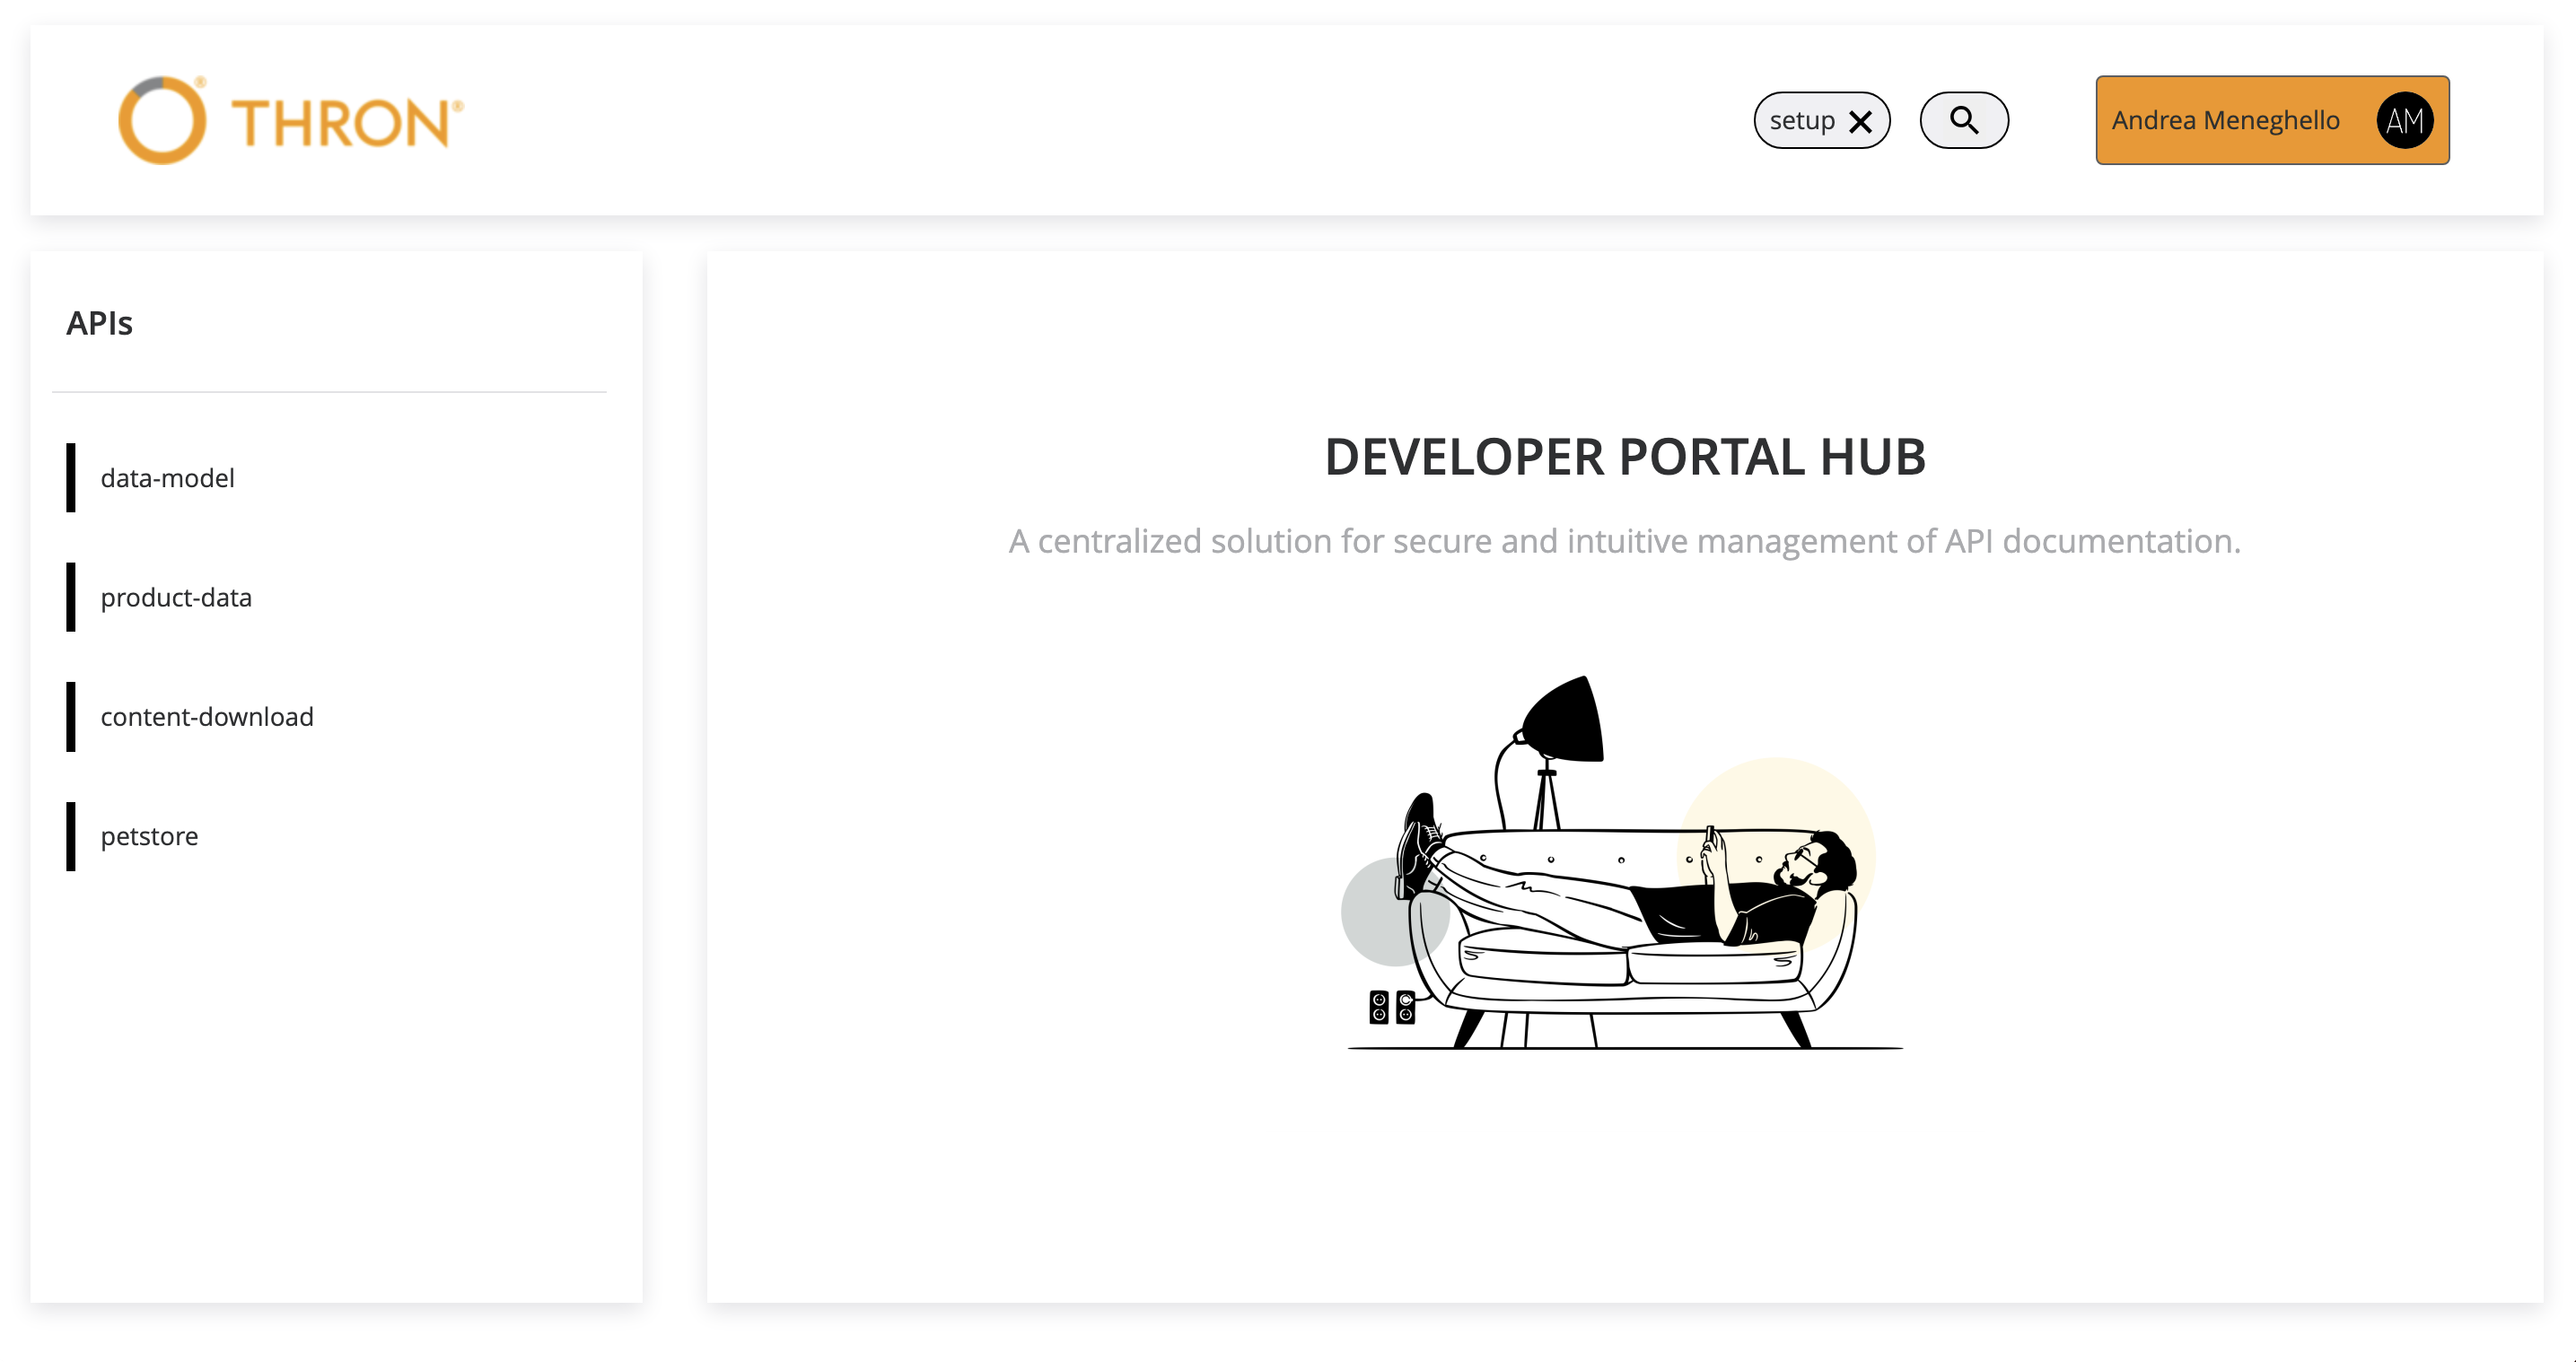
\includegraphics[width=0.6\textwidth, alt={Pagina principale dell'applicazione}]{images/frontend/HomeView.jpg}
  \caption{HomeView}\label{fig:home-view}
\end{figure}

Come la pagina di login, anche la pagina principale è stata sviluppata con un \textit{design responsive} (in figura~\ref{fig:home-view-responsive}).
Come si vede dall'immagine, si può notare che il menù laterale viene nascosto automaticamente e sarà accessibile cliccando l'apposito bottone a forma di \textit{hamburger}.

\begin{figure}[ht]
  \centering
  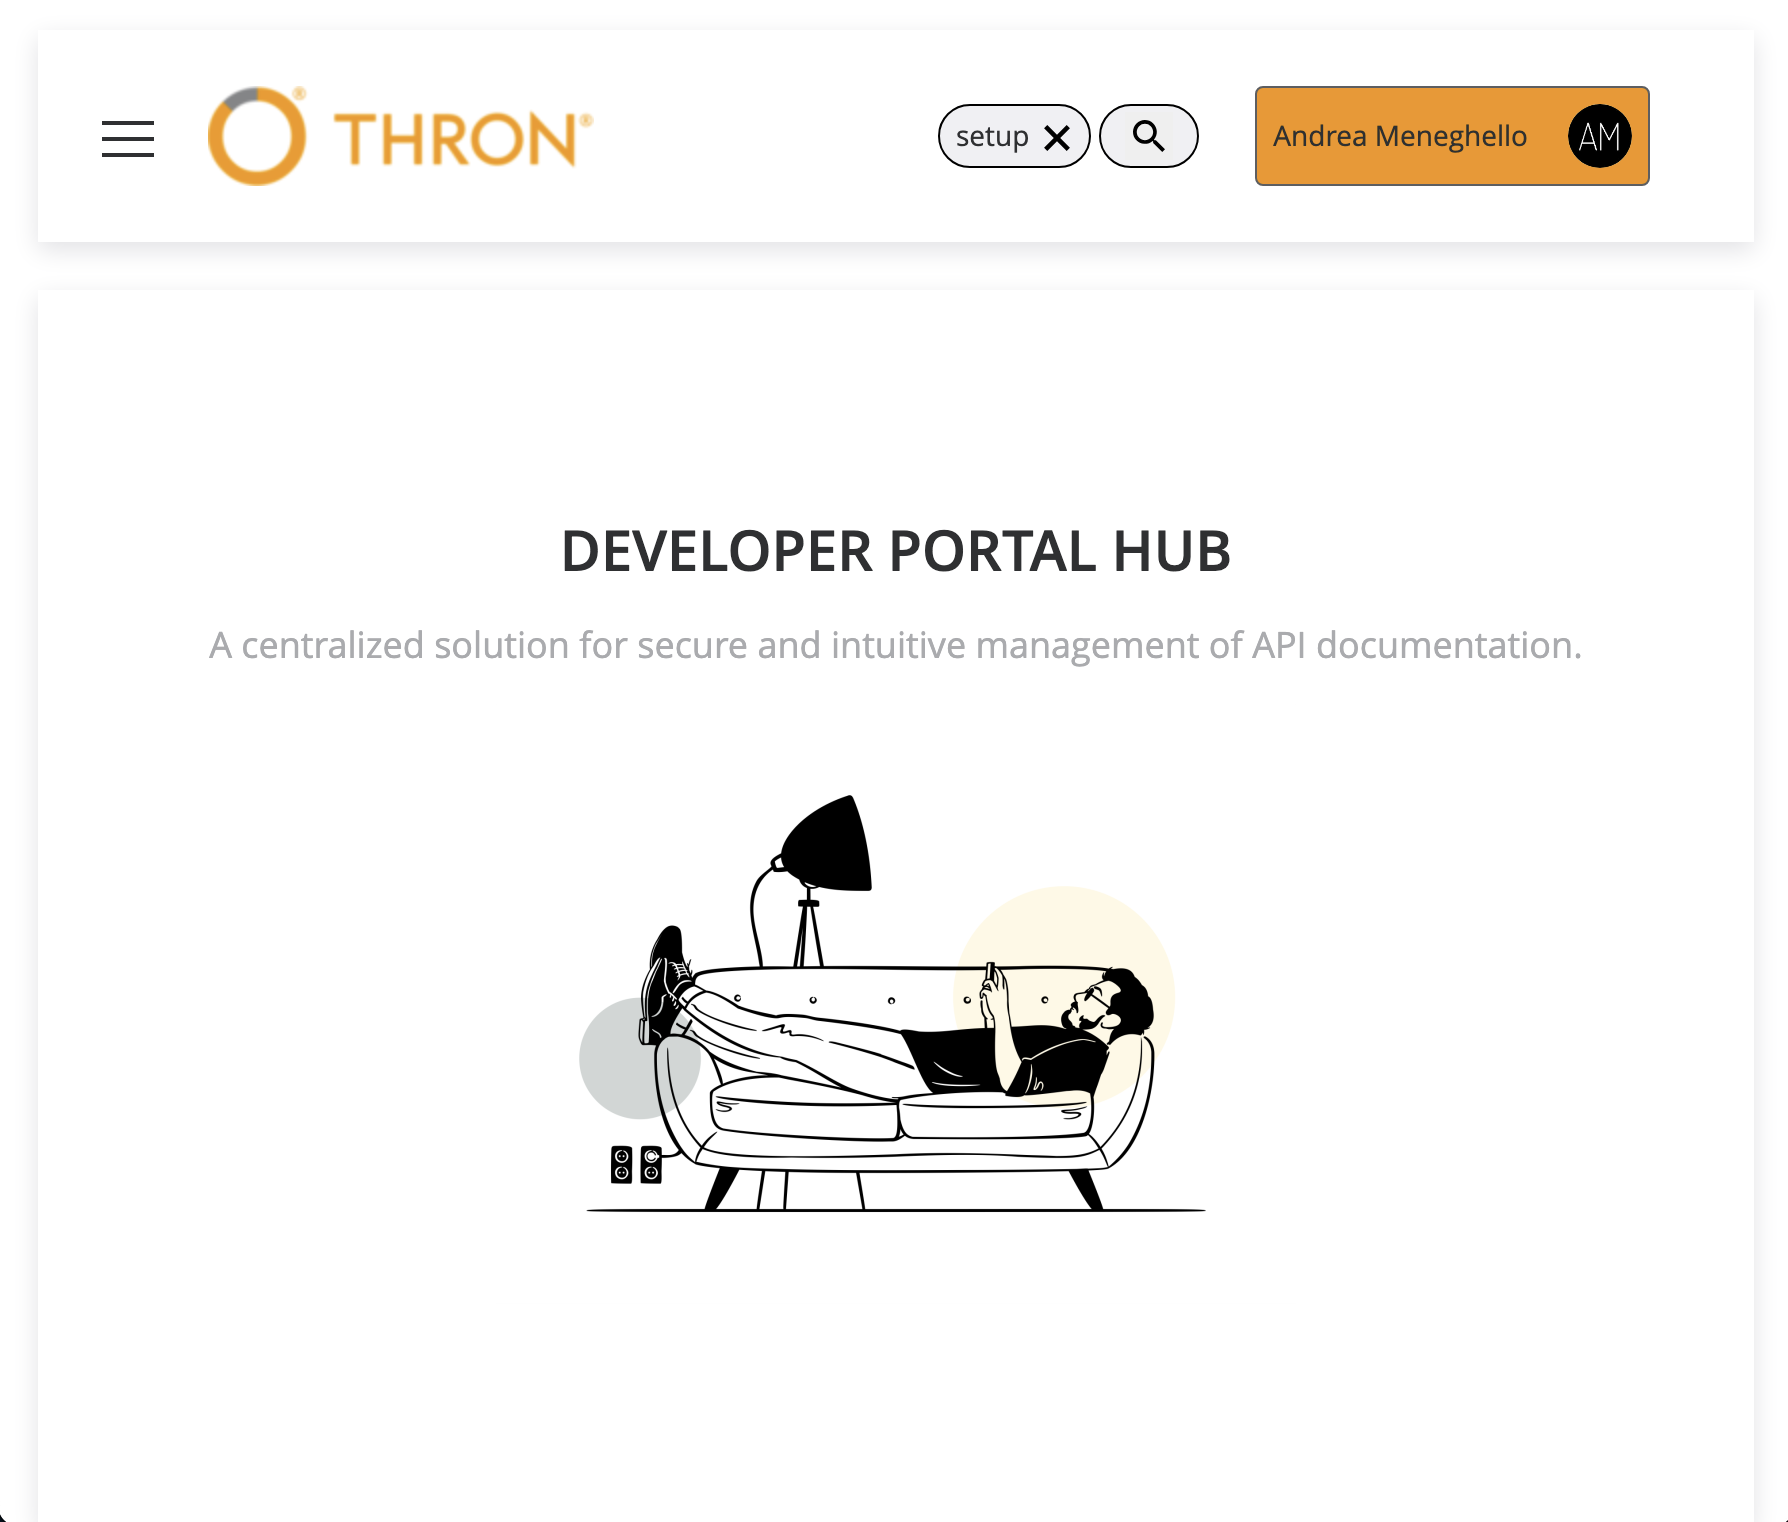
\includegraphics[width=0.5\textwidth, alt={Pagina principale responsive dell'applicazione}]{images/frontend/HomeViewRes.jpg}
  \caption{HomeView responsive}\label{fig:home-view-responsive}
\end{figure}


\subsubsection{NotFoundView}\label{subsubsec:not-found-view}
Quando un utente tenta di accedere ad una pagina non esistente, verrà reindirizzato automaticamente alla pagina di errore 404 (in figura~\ref{fig:not-found-view}).
La pagina consiste in un messaggio di errore con un'immagine, dove viene informato l'utente che la pagina richiesta non esiste.
Per tornare alla \textit{HomeView} basterà cliccare sul bottone \textit{Home} e si potrà continuare la navigazione all'interno del portale.

\begin{figure}[ht]
  \centering
  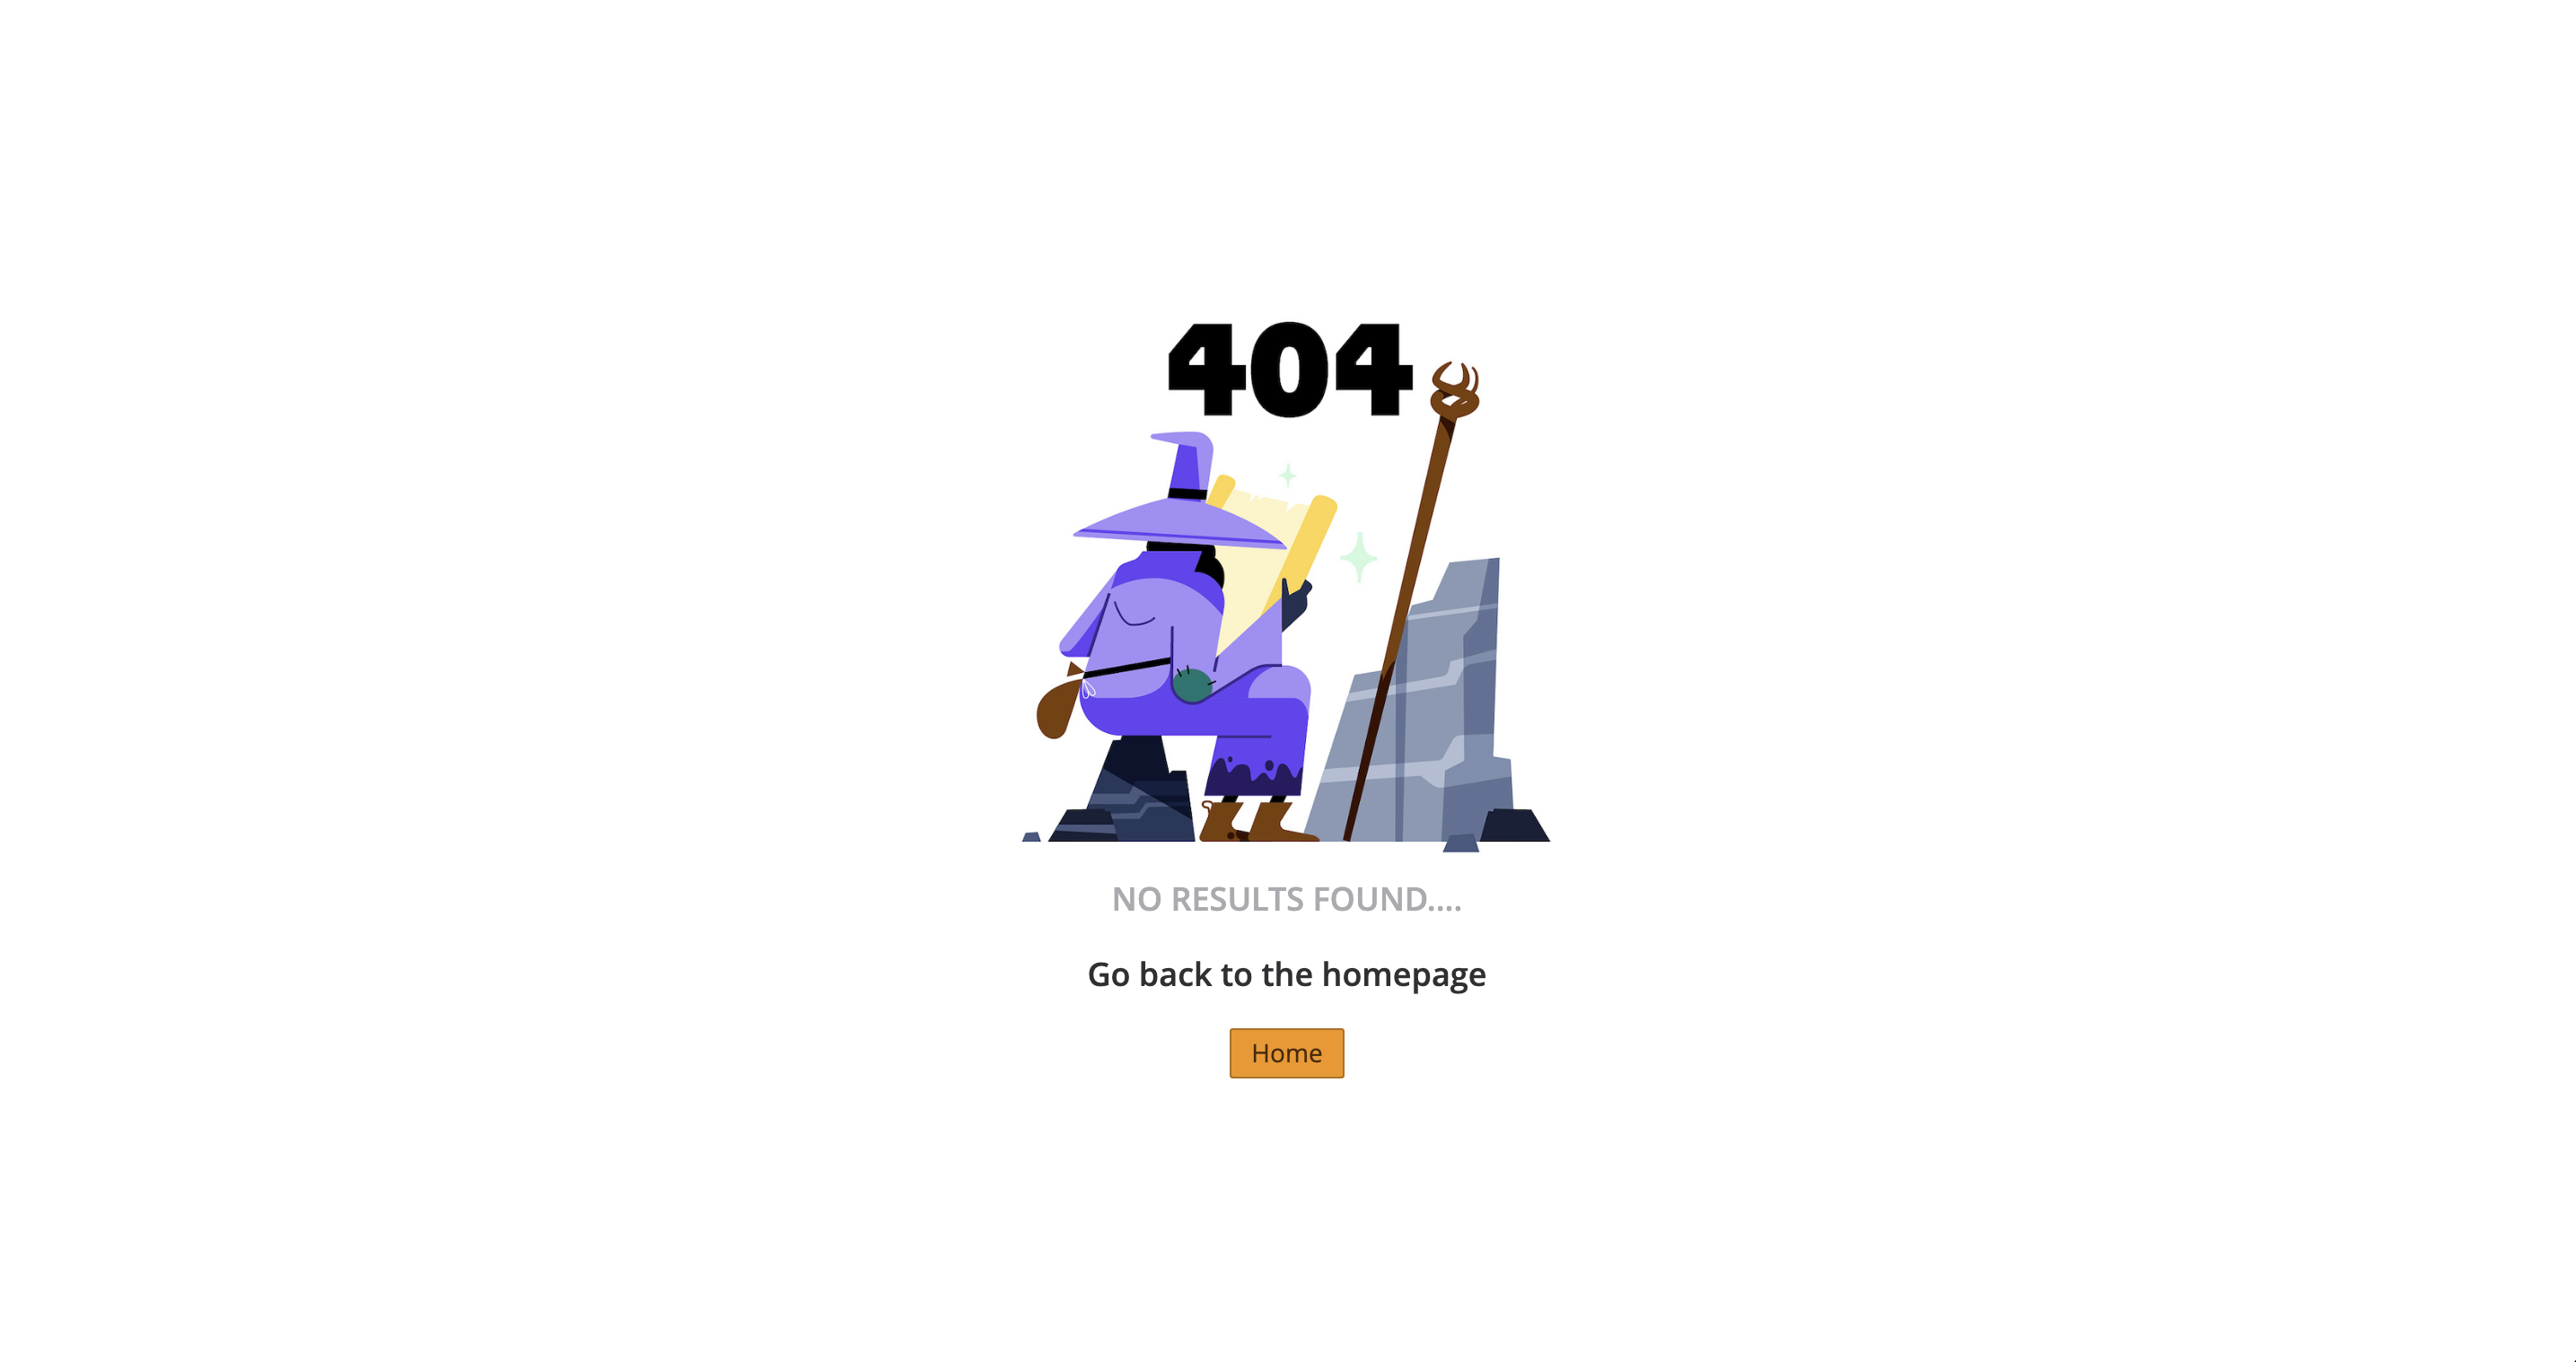
\includegraphics[width=0.6\textwidth, alt={Pagina di errore 404}]{images/frontend/NotFoundView.jpg}
  \caption{NotFoundView}\label{fig:not-found-view}
\end{figure}
\pagebreak
\subsection{Components}\label{subsec:components}

% Home
\subsubsection{HeaderNav}\label{subsubsec:header-nav}
Il componente rapppresenta la barra di navigazione superiore dell'applicazione (in figura~\ref{fig:header-nav-responsive}). Essa contiene il logo dell'applicazione, la \textit{chip} con il client-id
corrente, il bottone di ricerca e il \textit{popover} di logout. 
La barra viene sempre visualizzata una volta che l'utente ha effettuato il login all'interno del portale.\\
In caso di visualizzazione su schermi ridotti, l'\textit{HeaderNav} avrà un design responsive, dove viene aggiunto nell'estremità sinistra un bottone ad \textit{hamburger}
che permette di visualizzare la \textit{SideBar} a comparsa.

\begin{figure}[ht]
  \centering
  
\includegraphics[width=0.6\textwidth, alt={Barra di navigazione superiore con design responsive}]{images/frontend/HeaderRes.jpg}
  \caption{HeadearNav responsive}\label{fig:header-nav-responsive}
\end{figure}

\subsubsection{MainContent}\label{subsubsec:main-content}
Il componente rappresenta il contenuto principale dell'applicazione. Esso infatti contiene la struttura per visualizzare i dettagli di ogni API (in figura~\ref{fig:main-content}), tramite l'aiuto 
della libreria \textit{Swagger UI}.
La struttura segue il \textit{layout} di \textit{Swagger Editor} per motivi di semplicità e uniformità. Inizia con una descrizione iniziale, prosegue con la lista degli endpoint disponibili e conclude con l'elenco dei modelli.
I colori utilizzati sono uguali a quelli utilizzati in un comune \textit{Swagger Editor} per dare un senso di familiarità all'utente ed è stata una richiesta avanzata dal team.
Nell'angolo destro è stato aggiunto un bottone per il download della documentazione, che verrà discusso in seguito.
\begin{figure}[ht]
  \centering
  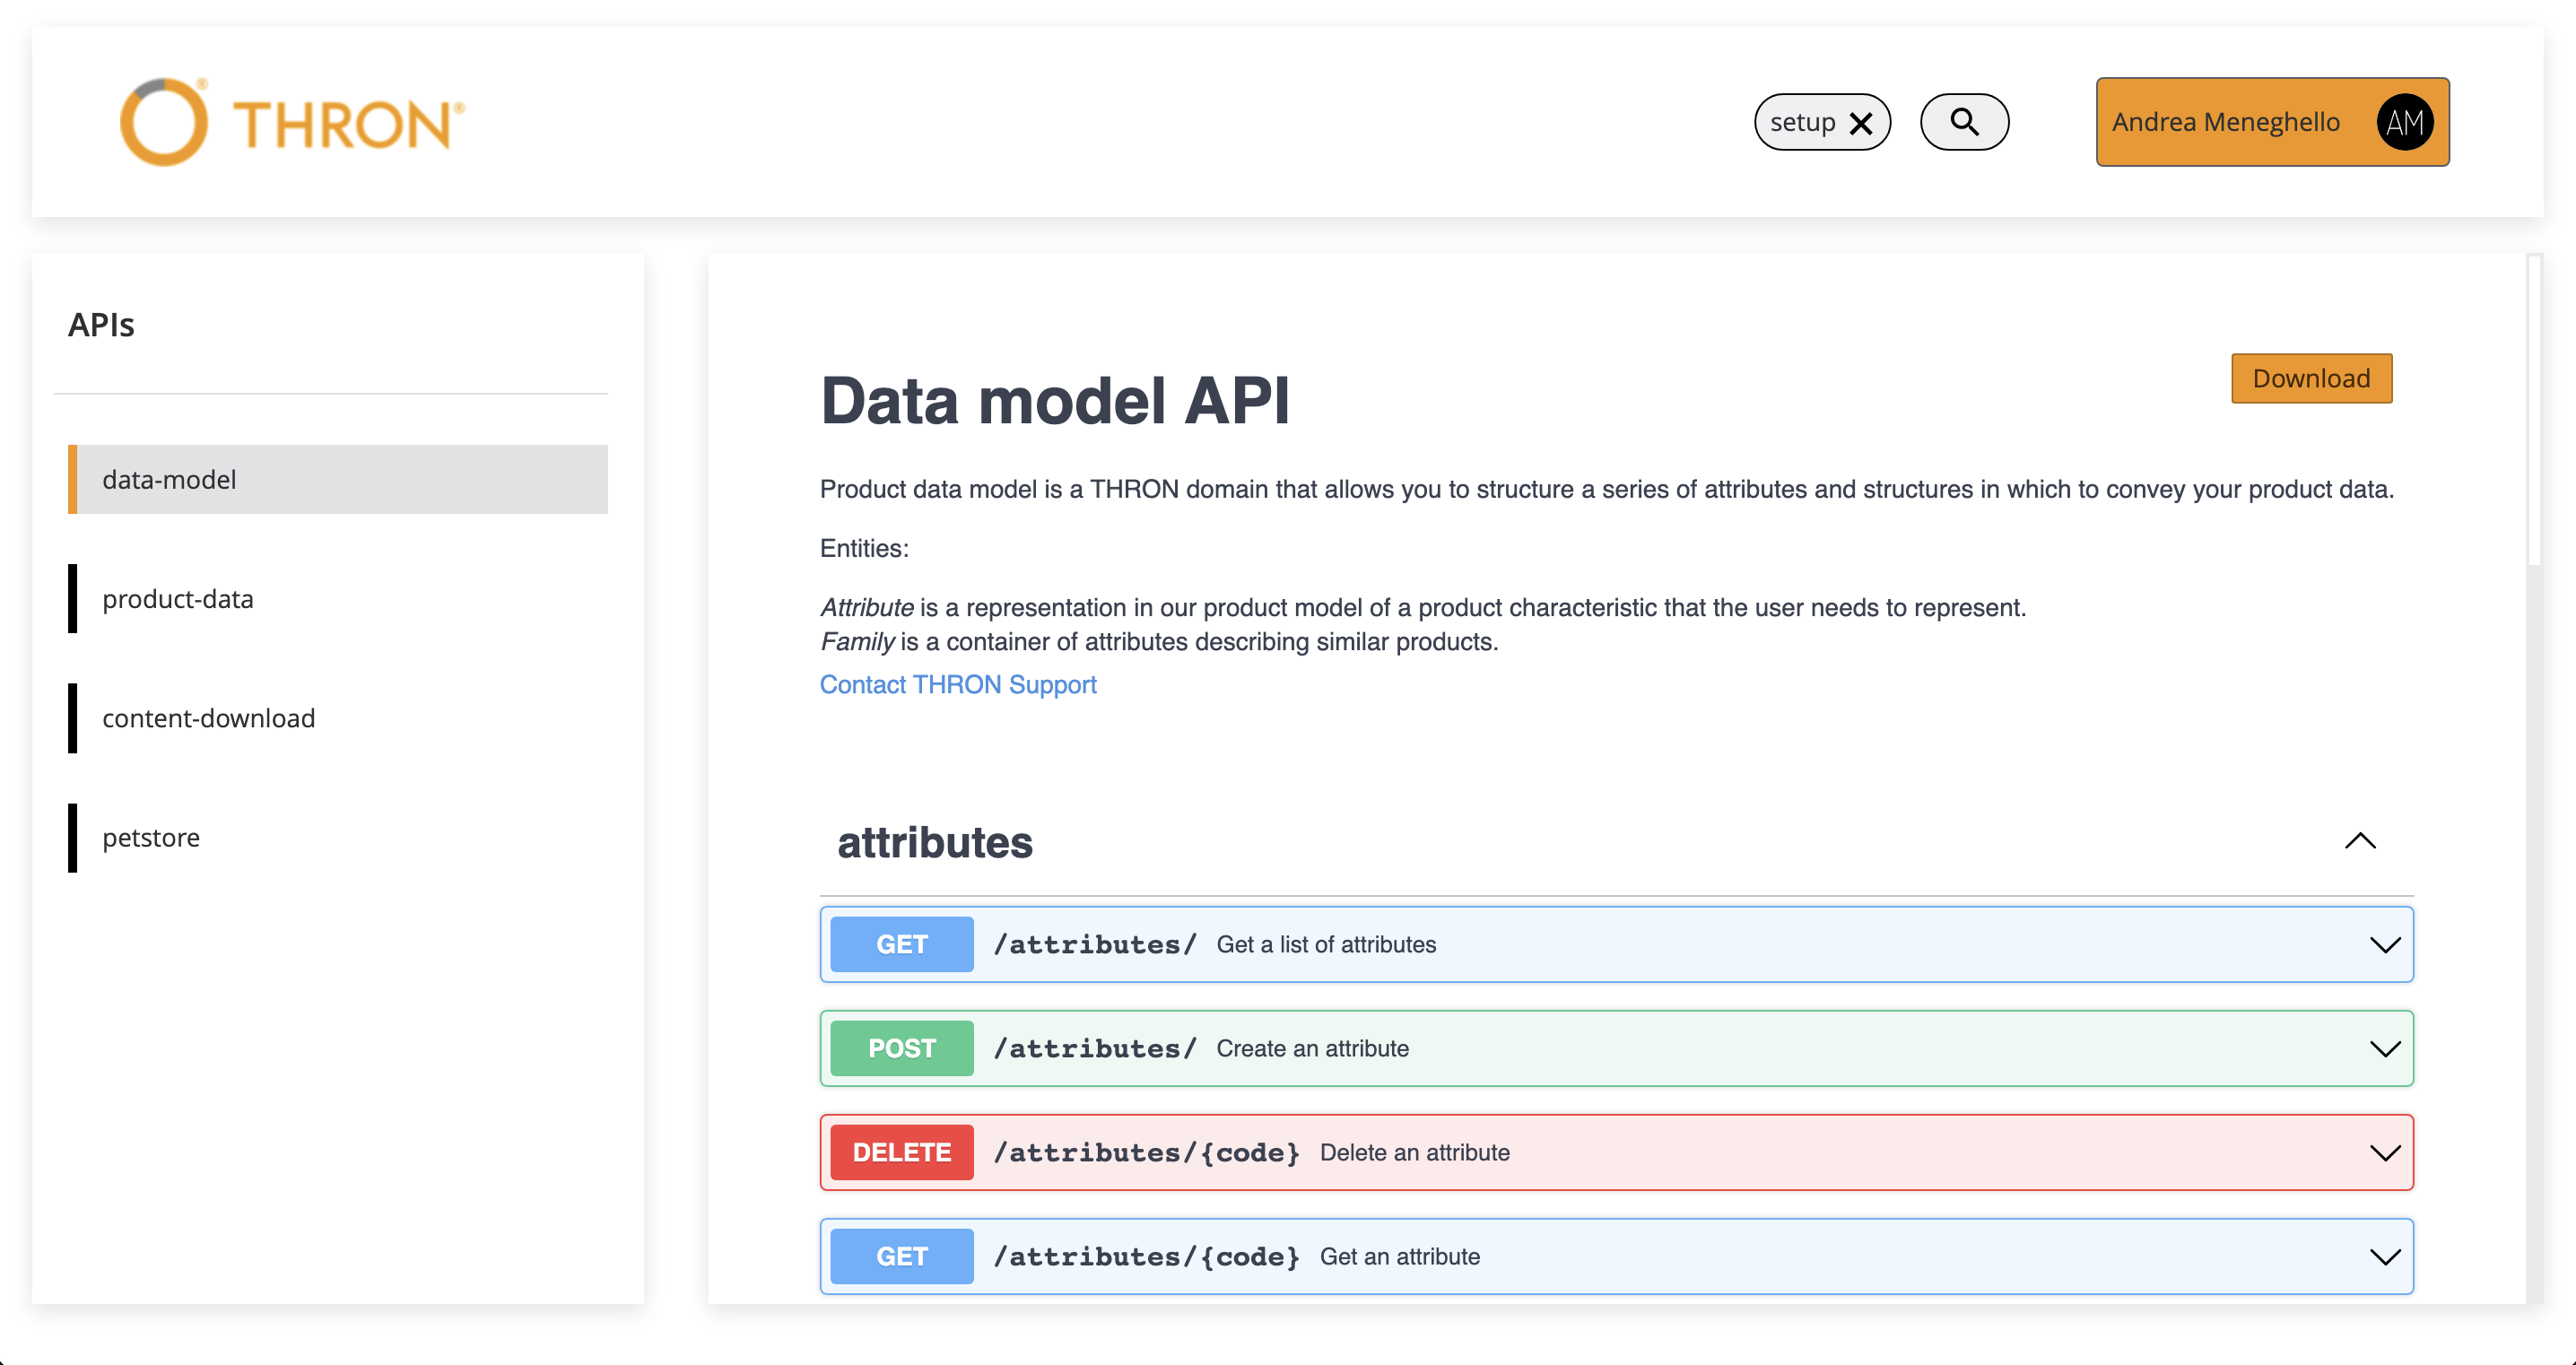
\includegraphics[width=0.6\textwidth, alt={Sezione per la visualizzazione dei dettagli di un API}]{images/frontend/DataModelView.jpg}
  \caption{MainContent}\label{fig:main-content}
\end{figure}
\pagebreak

Cliccando su uno degli endpoint disponibili, ci sarà una sezione dedicata per la visualizzazione dei dettagli di quest'ultimo (in figura~\ref{fig:try-it-out}).
I parametri e il \textit{Try it out} sono gestiti all'interno della \textit{utility SwaggerUtils} per una migliore suddivisione della logica.

\begin{figure}[ht]
  \centering
  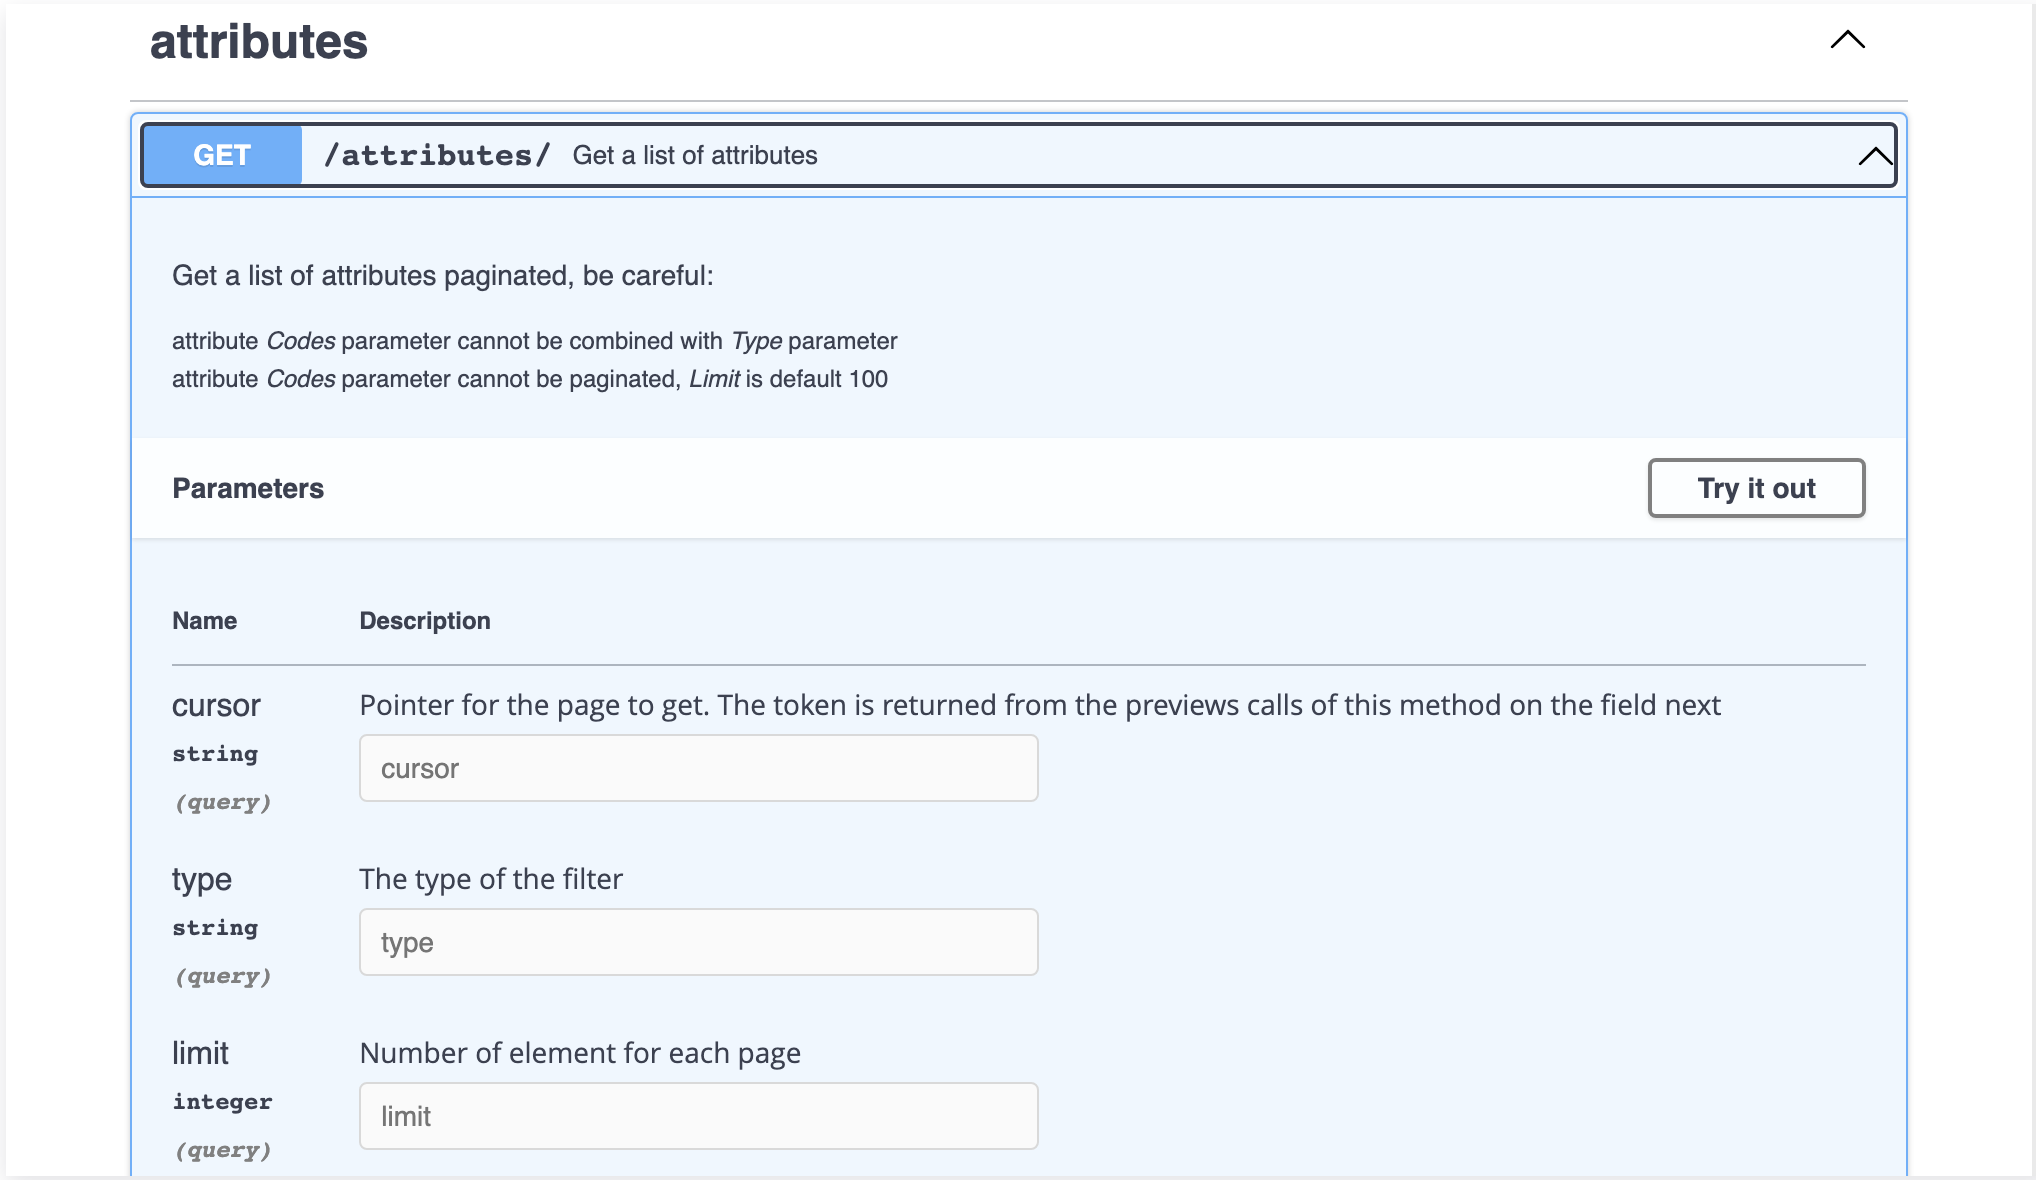
\includegraphics[width=0.6\textwidth, alt={Sezione try it out di un endpoint}]{images/frontend/TryItOut.jpg}
  \caption{Try it out di un endpoint}\label{fig:try-it-out}
\end{figure}

Inserendo i parametri e facendo quindi il \textit{try it out} verrà visualizzato il risultato della chiamata (in figura~\ref{fig:risposta-endpoint}).

\begin{figure}[ht]
  \centering
  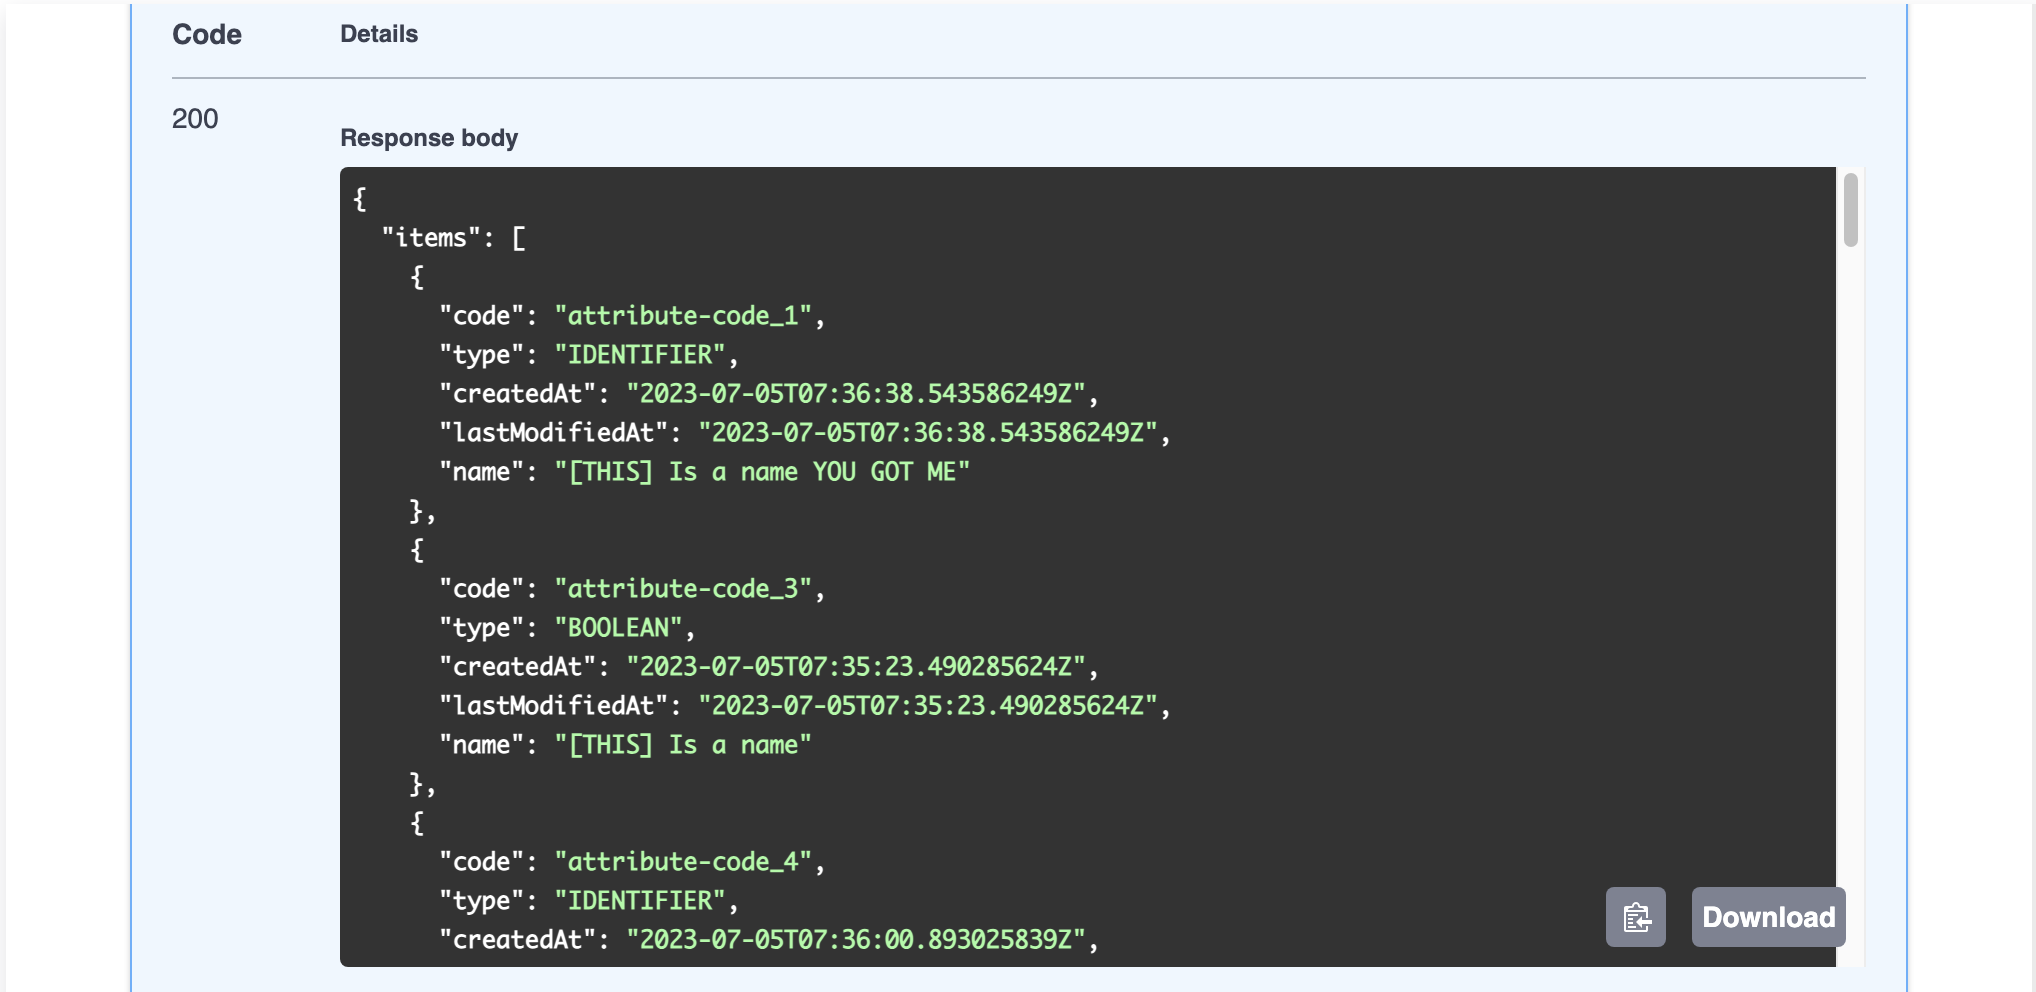
\includegraphics[width=0.6\textwidth, alt={Sezione per la visualizzazione della risposta di un endpoint}]{images/frontend/TryItOut3.jpg}
  \caption{Risposta di un endpoint}\label{fig:risposta-endpoint}
\end{figure}

Inoltre al di sotto sarà presente anche una lista delle possibili risposte che l'endpoint può restituire (in figura~\ref{fig:response-list}).

\begin{figure}[ht]
  \centering
  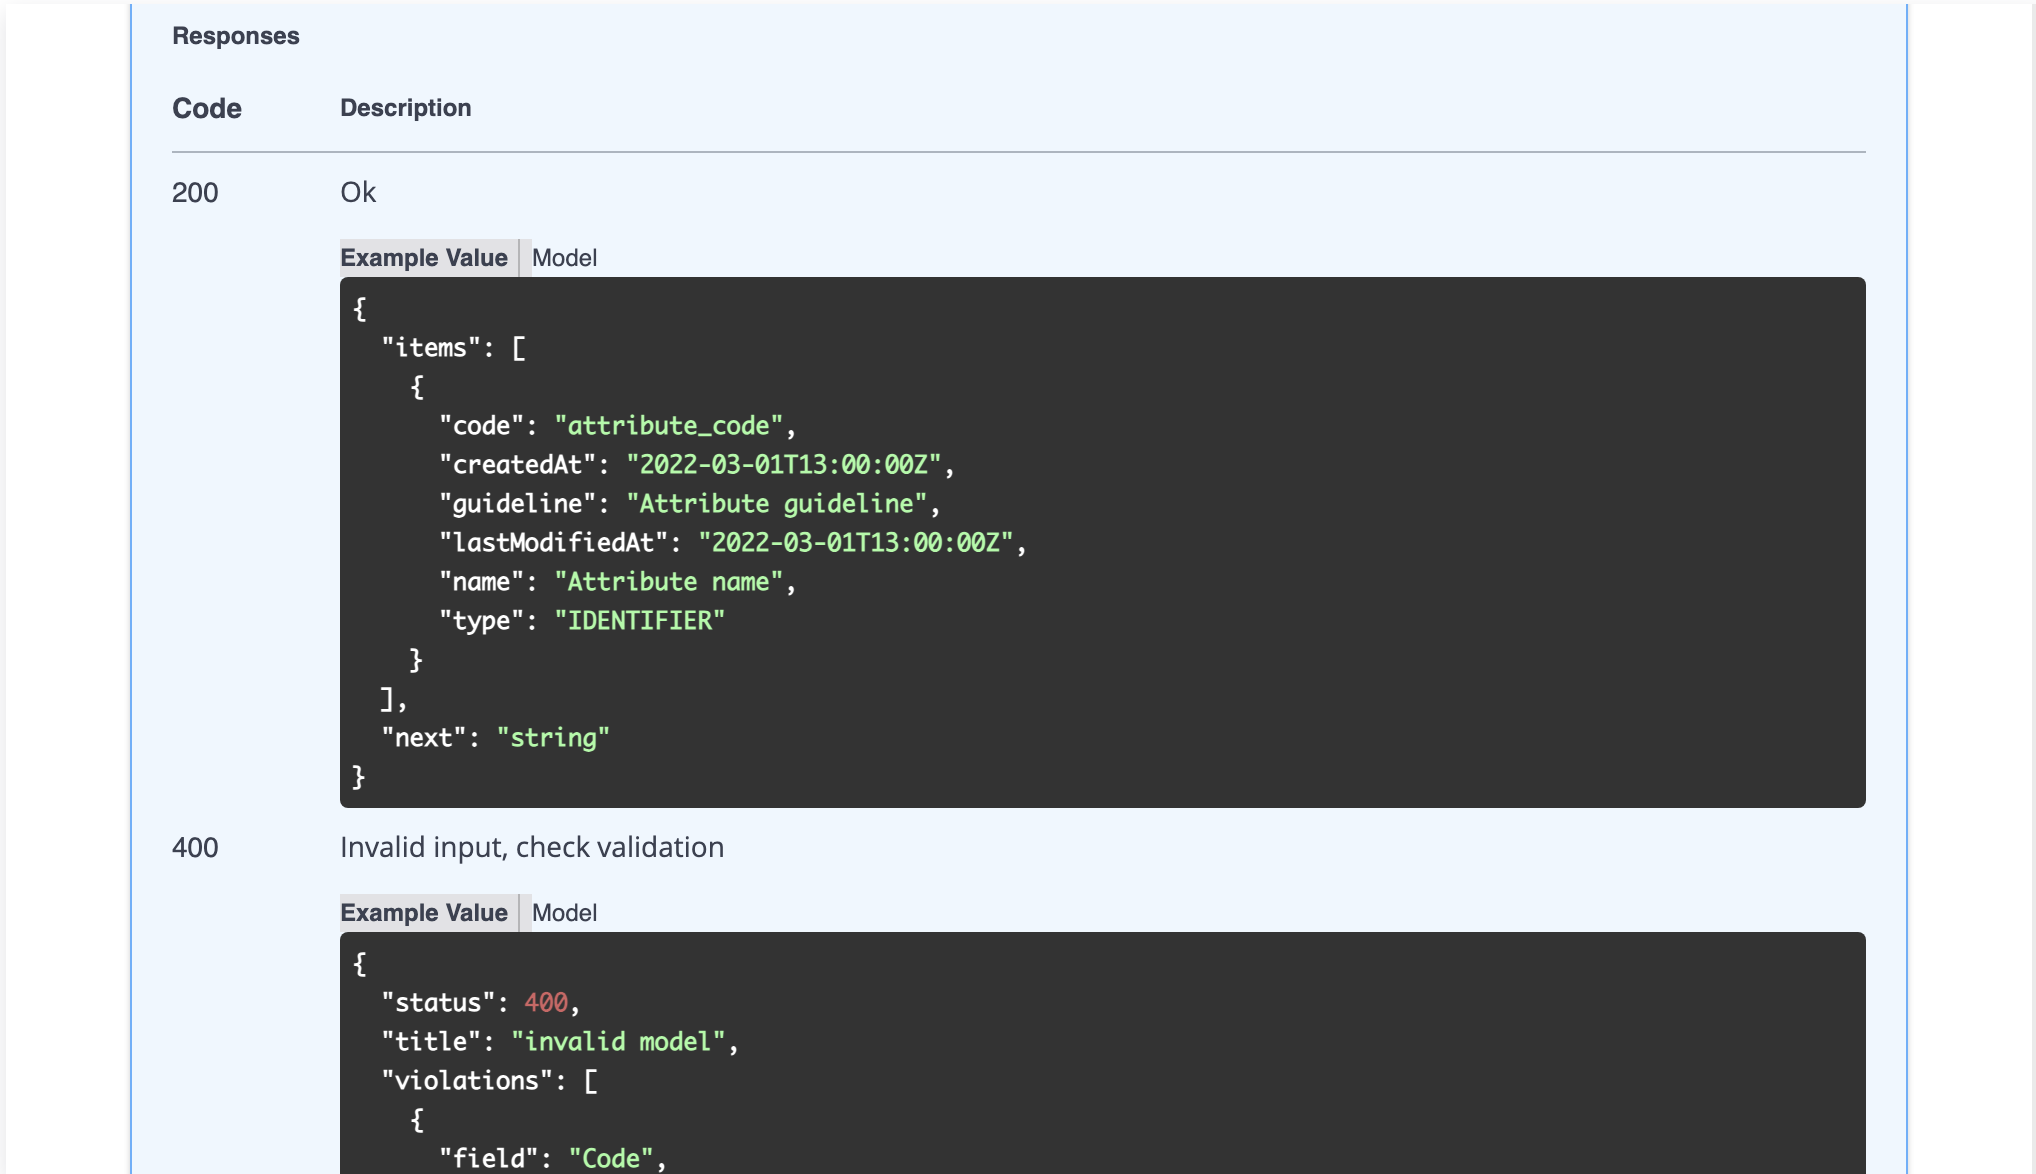
\includegraphics[width=0.6\textwidth, alt={Sezione per la visualizzazione delle possibili risposte di un endpoint}]{images/frontend/TryItOut4.jpg}
  \caption{Lista di risposte di un endpoint}\label{fig:response-list}
\end{figure}

\pagebreak

Nel caso di chiamate con necessità del parametro \textit{client-id}, è stato gestito tramite l'\textit{utility SwaggerUtils} l'\textit{autofill} di esso.
Infatti, il campo verrà compilato con il \textit{client-id} presente nella \textit{chip}, evitando che si inseriscano valori non presenti per 
quell'ambiente di sviluppo.


\subsubsection{SideBar}\label{subsubsec:side-bar}
Il componente rappresenta la barra di navigazione laterale dell'applicazione che contiene la lista di tutte le API disponibili nel portale (in figura~\ref{fig:side-bar-responsive}).
Attraverso la barra sarà possibile navigare tra le varie API, andando a visualizzare i dettagli di ognuna di esse. 
Il componente è stato sviluppato utilizzando un design responsive, che permette di visualizzare il contenuto in maniera ottimale anche su spazi ridotti, 
infatti il menù andrà a nascondersi automaticamente e sarà accessibile cliccando l'apposito bottone a forma di \textit{hamburger} situato nell'\textit{HeaderNav}.\\

\begin{figure}[ht]
  \centering
  \includegraphics[width=0.5\textwidth, alt={Design responsive della barra laterale}]{images/frontend/Sidebar.jpg}
  \caption{Design responsive SideBar}\label{fig:side-bar-responsive}
\end{figure}

\subsubsection{StartPage}\label{subsubsec:start-page}
% \gls{apig} è un portale che permette di consultare la documentazione delle API disponibili nel sistema.
Il componente rappresenta la pagina iniziale di benvenuto dell'applicazione ed è la prima schermata che l'utente visualizza dopo aver effettuato il login con successo.
Essa contiene il nome del portale, una breve descrizione e un'immagine. Per iniziare la navigazione nel portale, basterà usare la \textit{SideBar}.

\subsubsection{SwaggerLoader}\label{subsubsec:swagger-loader}
Il componente rappresenta il loader di caricamento per il \textit{MainContent} (in figura~\ref{fig:swagger-loader}). 
Esso rappresenta un caricamento di stile \textit{skeleton}, ovvero un caricamento di contenuto che simula il contenuto finale, mentre questo viene caricato, attraverso un sfondo dinamico grigio.
Il componente ha la stessa struttura del \textit{MainContent}, quindi segue lo stesso design responsive.
Il loader sarà visibile ogni volta che l'utente clicca su una delle API disponibili nella \textit{SideBar}, e scomparirà una volta che il contenuto sarà caricato correttamente.

\begin{figure}[ht]
  \centering
  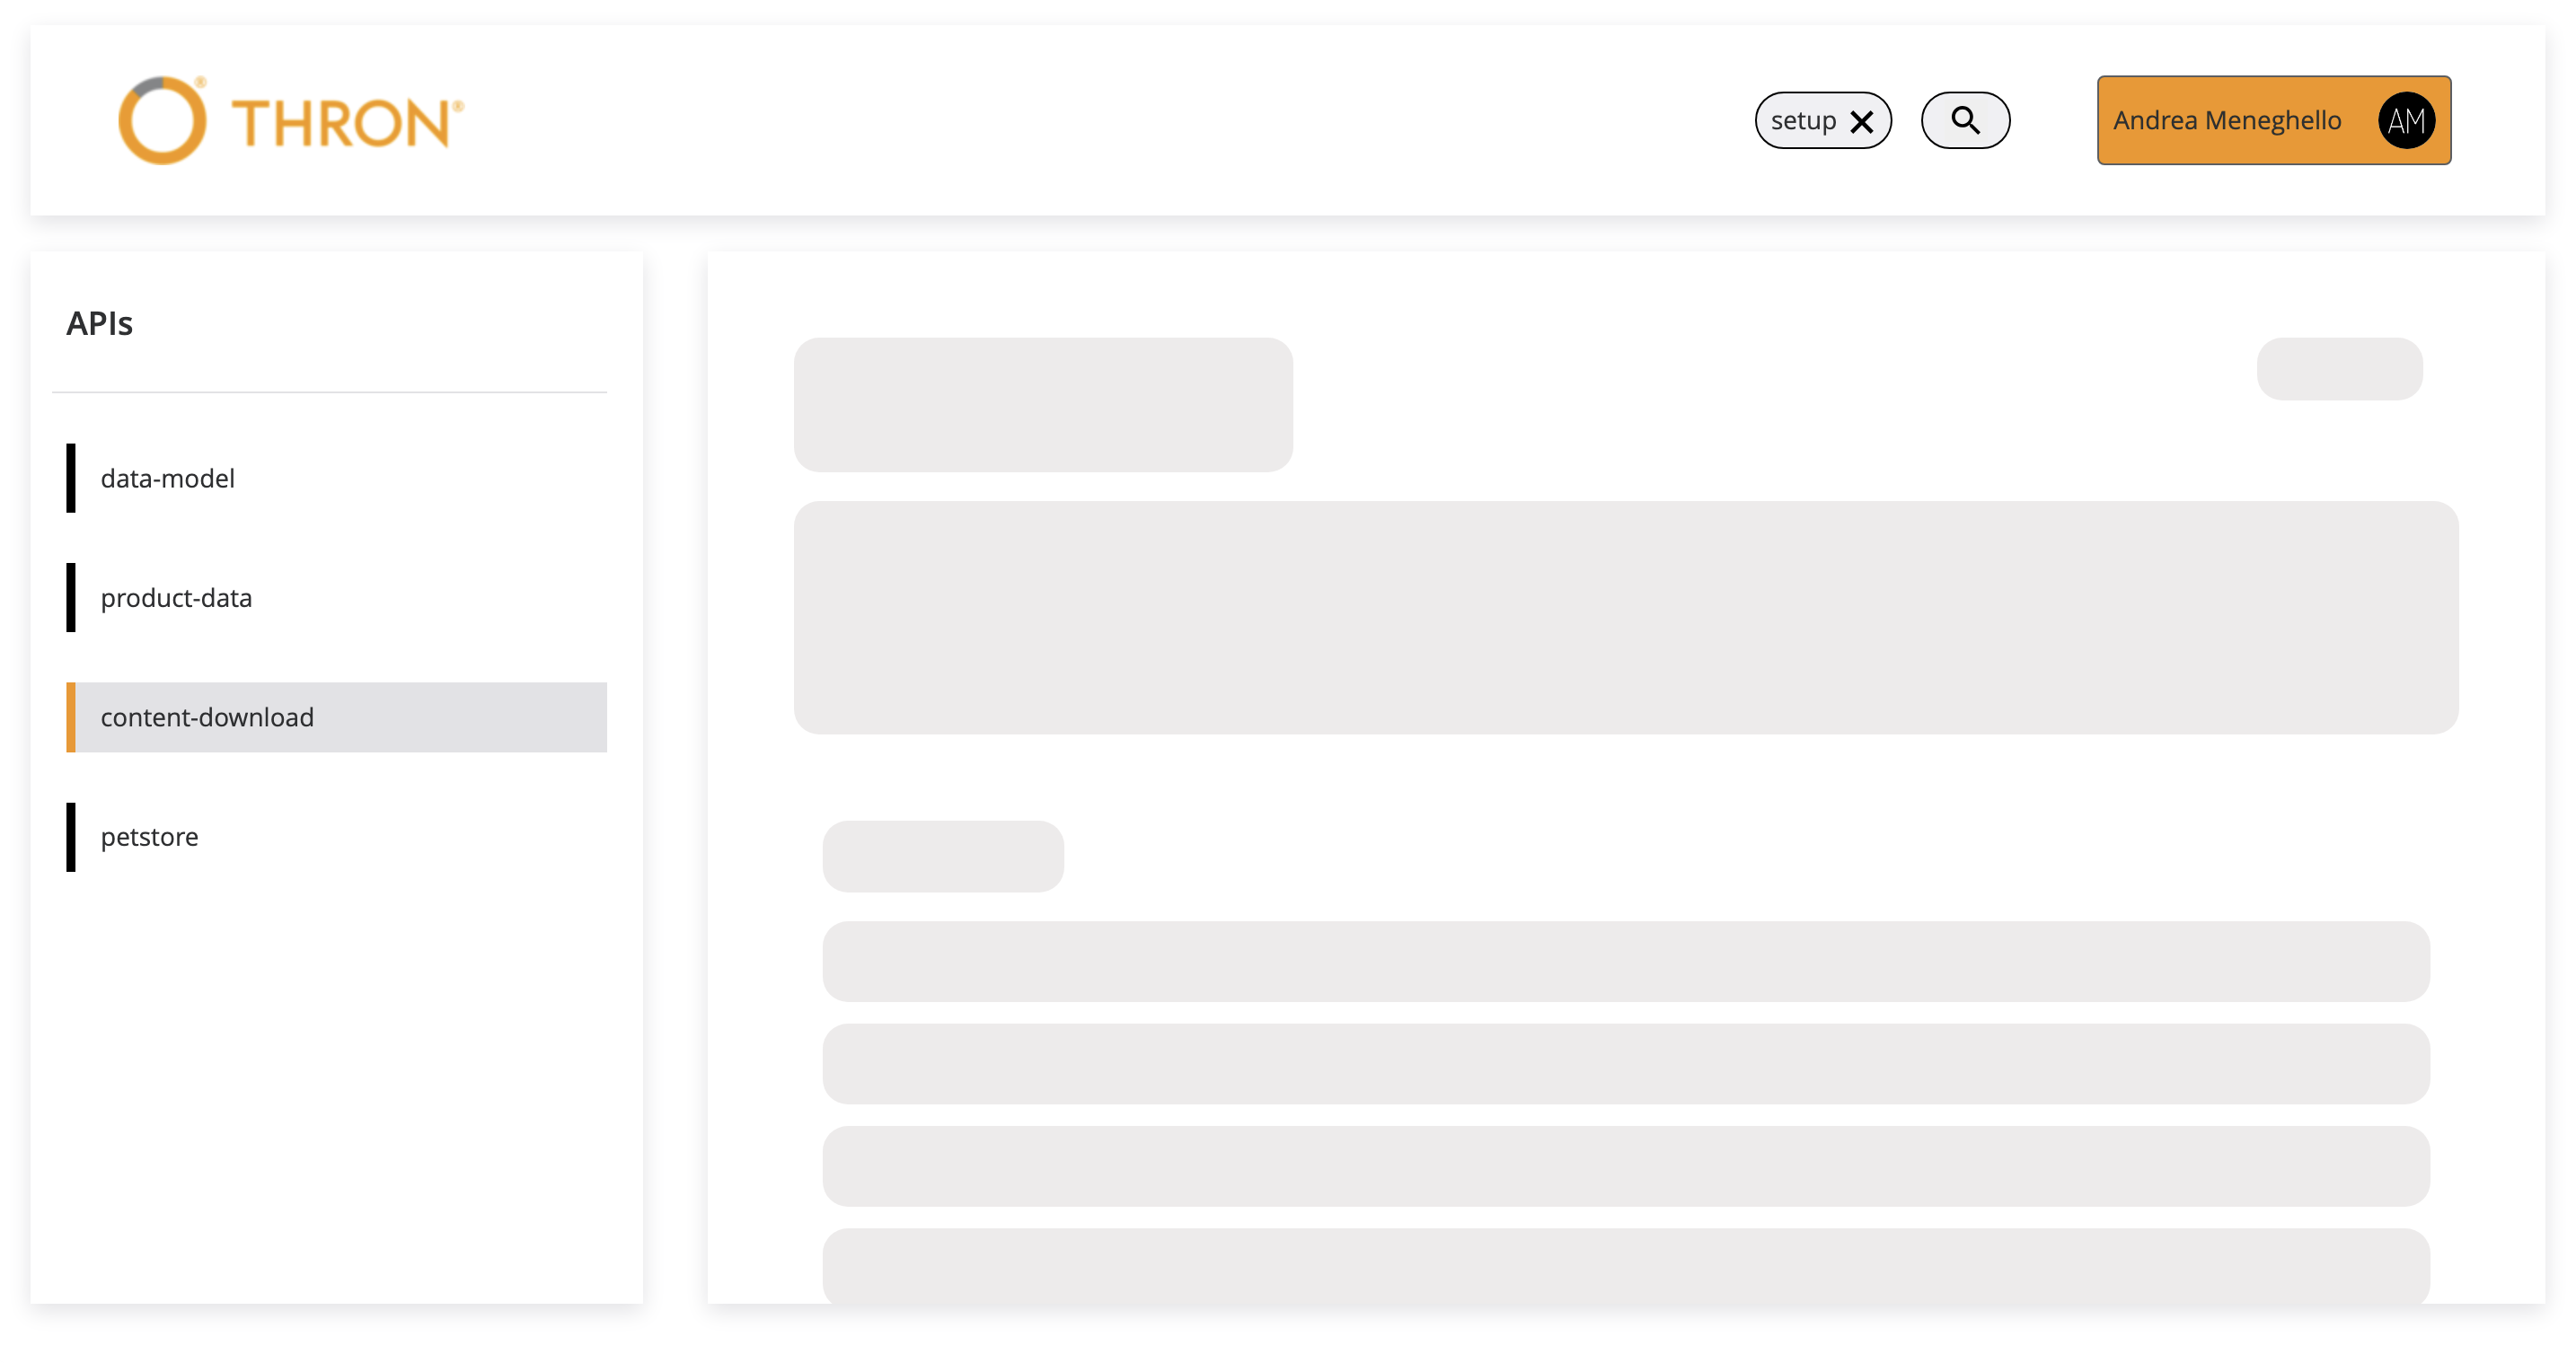
\includegraphics[width=0.6\textwidth, alt={Skeleton loader di caricamento per contenuto principale}]{images/frontend/SwaggerLoader.jpg}
  \caption{SwaggerLoader}\label{fig:swagger-loader}
\end{figure}

% \pagebreak
\subsubsection{DownloadButton}\label{subsubsec:download-button}
Il componente rappresenta il bottone di download presente in ogni pagina di dettaglio dell'API specifica. Esso è stato sviluppato rispettando il \textit{design system}
aziendale, infatti non è un componente \textit{custom} creato da zero, ma è stato sviluppato utilizzando il componente \textit{Button} della libreria \textit{Components} THRON.
Il componente da la possibilità di scegliere la grandezza, il testo del bottone e icone da visualizzare.
Il componente permette all'utente di scaricare la documentazione dell'API in formato \textit{.yaml}, con un nome predefinito a seconda 
del servizio scaricato. Una volta cliccato, andrà ad aprire una finestra secondaria del browser, e il file verrà scaricato automaticamente.\\

\subsubsection{LogoutButton}\label{subsubsec:logout-button}
Il componente rappresenta il bottone di logout presente nella barra di navigazione superiore 
dell'applicazione ed è stato sviluppato rispettando il \textit{design system} 
aziendale, infatti utilizza la libreria \textit{THRON Components} (in figura~\ref{fig:logout-button}).
Nello specifico è stato chiamato bottone per comodità, ma in realtà si tratta di un \textit{popover}, ovvero un componente a tendina che si apre
tramite l'\textit{hover} del mouse. Esso permette all'utente di effettuare il logout dal portale tramite un \textit{pop-up}, con successivo reindirizzamento
alla pagina di login.

\begin{figure}[ht]
  \centering
  
\includegraphics[width=0.5\textwidth, alt={Popover per il logout dall'applicazione}]{images/frontend/logout.jpg}
  \caption{LogoutButton}\label{fig:logout-button}
\end{figure}

% Login
\subsubsection{LoginButton}\label{subsubsec:login-button}
Il componente rappresenta il bottone di accesso al portale presente nella pagina di login dell'applicazione. Esso è stato sviluppato rispettando il \textit{design system} aziendale.
Il seguente bottone aprirà un \textit{pop-up} dove sarà possibile inserire le credenziali (e-mail e password) per effettuare l'accesso tramite \textit{Microsoft} 365.
Una volta effettuato il login, l'utente verrà reindirizzato alla pagina principale del portale.

% Components
\subsubsection{SearchButton}\label{subsubsec:search-button}
Il componente rappresenta il bottone di ricerca presente nella barra di navigazione superiore dell'applicazione.
Si tratta di un componente \textit{custom} creato da me, utilizzato per aprire la barra di ricerca globale del portale. 

\subsubsection{SearchBar}\label{subsubsec:search-bar}
Il componente rappresenta la barra di ricerca globale dell'applicazione (in figura~\ref{fig:search-bar}). 
Essa consiste in una barra dove poter inserire il \textit{client-id} o il nome dell'\textit{API} da cercare,
con un'icona di ricerca a fianco. Per una migliore esperienza di ricerca, è necessario utilizzare il componente insieme al componente \textit{autocomplete} descritto in seguito.
Infatti i componenti insieme, costituiscono la ricerca all'interno del portale. Inoltre La \textit{SearchBar} è accessibile anche tramite tastiera,
infatti tramite il comando \textit{Ctrl + B} sarà possibile aprire la barra di ricerca.\\

\begin{figure}[ht]
  \centering
  
\includegraphics[width=0.6\textwidth, alt={Barra di ricerca globale dell'applicazione}]{images/frontend/SearchBar.jpg}
  \caption{SearchBar}\label{fig:search-bar}
\end{figure}
\pagebreak

\subsubsection{Autocomplete}\label{subsubsec:autocomplete}
Il componente rappresenta l'elenco dei risultati visualizzato sotto la barra di ricerca dell'applicazione (in figura~\ref{fig:autocomplete}).
Essa consiste in una lista di suggerimenti dinamici che vengono visualizzati in base al testo inserito dall'utente. 
In caso il campo di ricerca della \textit{SearchBar} sia vuoto, verrà mostrata la lista degli ultimi quattro termini cercati, se presenti.
In caso contrario, quando è presente un termine nella barra di ricerca, verrà visualizzata una lista di suggerimenti divisa per categoria.
Nel caso in cui la ricerca non abbia prodotto risultati, verrà visualizzato un messaggio di errore, gestito tramite il componente \textit{SnackBar} descritto in seguito.\\
La logica della ricerca è completamente sviluppata lato \textit{backend} per estrapolare il componente di ricerca e renderlo riutilizzabile in altri progetti.
Essendo un componente \textit{custom}, ho aggiunto la possibilità di navigare il menù e selezionare un suggerimento tramite tastiera, funzionalità 
obbligatoria per rendere la ricerca accessibile anche a persone con disabilità.\\
Dopo aver selezionato un suggerimento, verrà aperta la pagina di dettaglio dell'API corrispondente se l'utente ha scelto un'API specifica.  In caso contrario, il client-id corrente verrà impostato e la Chip verrà aggiornata.
Il componente infine supporta la gestione di più liste di elementi per la ricerca globale, non limitandosi a soli due elenchi. Questo significa che è possibile avere un numero variabile di liste di elementi con cui effettuare la ricerca globale. 

\begin{figure}[ht]
  \centering
  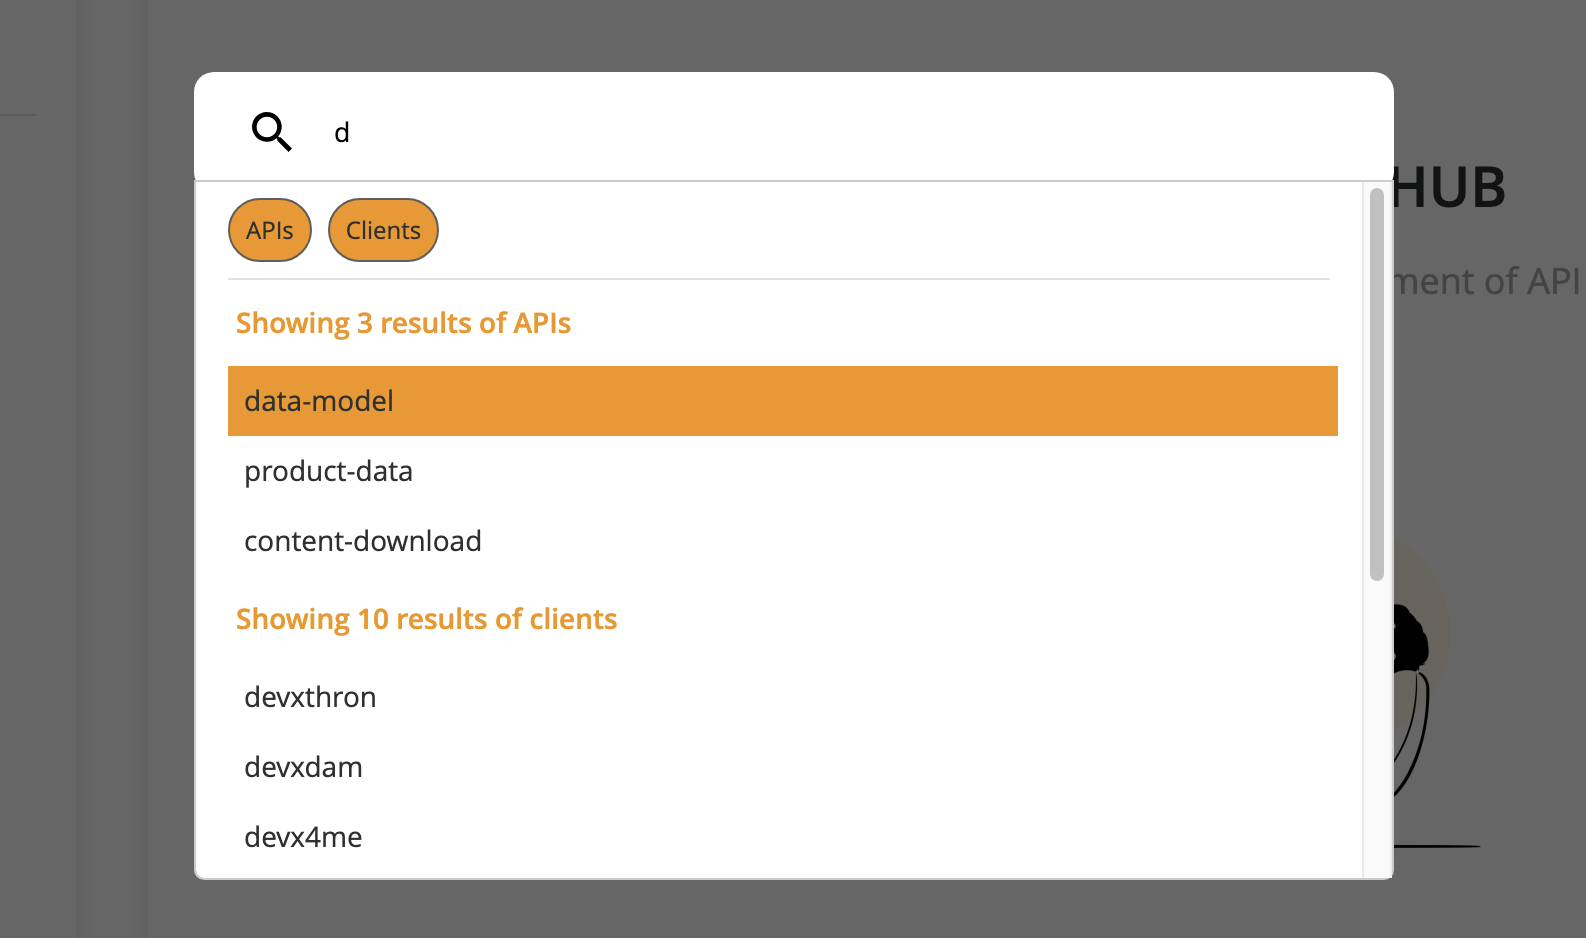
\includegraphics[width=0.6\textwidth, alt={Componente che si occupa della lista dinamica di risultati}]{images/frontend/SearchBar2.jpg}
  \caption{Autocomplete}\label{fig:autocomplete}
\end{figure}
\pagebreak
\subsubsection{Chip}\label{subsubsec:chip}
Il componente rappresenta la \textit{chip} situata nella barra di navigazione superiore dell'applicazione (in figura~\ref{fig:chip}).
Essa è utile a visualizzare il \textit{client-id} corrente, ovvero il \textit{client-id} che l'utente ha selezionato tramite la barra di ricerca globale.
Se l'utente non ha ancora effettuato alcuna selezione, verrà visualizzato il \textit{client-id} predefinito dell'ambiente di sviluppo.
Inoltre è possibile reimpostare il \textit{client-id} corrente cliccando sull'icona di reset a forma di \textit{X}, riportandolo al valore di default.
In caso il \textit{client-id} fosse già al valore predefinito, verrà visualizzato un messaggio di errore tramite il componente \textit{SnackBar} descritto in seguito.

\begin{figure}[ht]
  \centering
  
\includegraphics[width=0.3\textwidth, alt={Chip contenente il client id corrente}]{images/frontend/Chip.jpg}
  \caption{Chip}\label{fig:chip}
\end{figure}


\subsubsection{Filter}\label{subsubsec:filter}
Il componente rappresenta il bottone per filtrare la lista dei risultati della ricerca, all'interno del componente \textit{Autocomplete}.
Quando il bottone viene cliccato, lo sfondo risulta bianco e verrà visivamente nascosta la lista corrispondente al filtro cliccato.
Cliccando di nuovo sullo stesso filtro, il bottone tornerà arancione e verrà  mostrata la lista corrispondente al filtro cliccato.


\subsubsection{OptionList}\label{subsubsec:option-list}
Il componente rappresenta la lista di opzioni generiche, visualizzate all'interno della SideBar. Nel mio progetto, è stata utilizzata per visualizzare la lista
di tutte le \textit{API} disponibili nel sistema. 

\subsubsection{OptionListItem}\label{subsubsec:option-list-item}
Il componente rappresenta un singolo elemento della lista di opzioni generiche, visualizzate all'interno della SideBar. Nel mio progetto, un'\textit{item} rappresenta una singola \textit{API}.
Andando a cliccare un'opzione, verrà aperta la pagina di dettaglio dell'\textit{API} selezionata.

\subsubsection{SnackBar}\label{subsubsec:snack-bar}
Il componente rappresenta la \textit{snack-bar} dell'applicazione usata per la visualizzazione di messaggi di errore o di successo (in figura~\ref{fig:snack-bar}).
All'interno del portale è utilizzata per comunicare all'utente che un termine cercato non ha prodotto risultati, che il \textit{client-id} è stato resettato con successo
oppure per informare l'utente che il \textit{client-id} è già al valore di default.
Ho creato il componente con l'idea di renderlo riutilizzabile per diversi scopi, infatti è possibile modificare vari aspetti come il colore, il tipo di icona,
la durata del messaggio, il testo da visualizzare, la posizione del componente e la dimensione del componente.

\begin{figure}[ht]
  \centering
  
\includegraphics[width=0.5\textwidth, alt={Snackbar di errore}]{images/frontend/SnackBar1.jpg}
  \caption{SnackBar}\label{fig:snack-bar}
\end{figure}

\subsubsection{Loader}\label{subsubsec:loader}
Il seguente componente rapppresenta il sistema di caricamento principale dell'applicazione (in figura~\ref{fig:loader}).
Esso rappresenta un caricamento stile \textit{skeleton}, ovvero un caricamento che simula la presenza di contenuti, mentre questi vengono caricati, attraverso 
uno sfondo dinamico grigio.
Il componente è stato utilizzato per il caricamento della struttura della pagina, ovvero è composto da tre sezioni: \textit{HeaderNav}, \textit{SideBar} e
\textit{MainContent}. Il loader sarà visibile subito dopo aver effettuato il login o quando la pagina viene ricaricata, e scomparirà una volta che i dati saranno stati caricati correttamente.
Inoltre il componente è stato sviluppato utilizzando un design responsive, infatti seguirà la stessa struttura della pagina, andando a nascodere la sezione 
\textit{SideBar} in caso di schermi di piccole dimensioni.
Ho preferito utilizzare un caricamento di tipo \textit{skeleton} rispetto ad un classico \textit{loader} circolare, perchè secondo me migliora l'esperienza utente 
conferendo una sensazione migliore durante l'attesa del caricamento dei dati.

\begin{figure}[ht]
  \centering
  
\includegraphics[width=0.6\textwidth, alt={Skeleton loader di caricamento principale dell'applicazione}]{images/frontend/Loader.jpg}
  \caption{Loader}\label{fig:loader}
\end{figure}
\pagebreak

\section{Codifica backend}\label{sec:codifica-backend}

\subsection{Middleware}\label{subsec:middleware}
Il middleware è un meccanismo che permette di eseguire delle operazioni specifiche durante il ciclo di vita di una richiesta HTTP. 
Nel mio caso ho utilizzato questa funzionalità per svolgere della logica prima che la richiesta venga inoltrata al Controller e generi una risposta.
Il middleware è stato utilizzato per due scopi principali: la validazione del \textit{token JWT} di autenticazione e l'acquisizione del \textit{supertoken} utile per eseguire delle chiamate.
Basandoci sul ciclo di vita, il middleware intercetta le richieste, effettua le funzionalità appena descritte e successivamente inoltra la richiesta al Controller che si occuperà di restituire una risposta.
Quindi ogni chiamata verso gli \textit{endpoint} che ho sviluppato e che verranno descritti in seguito, passerà prima dal middleware. Questo perchè sono andato a specificare
nel modulo principale dell'applicazione le rotte che devono essere gestite dal \textit{middleware}, ovvero i controller di \textit{client-id}, \textit{API} e \textit{search}.

\subsubsection{Validazione token JWT}
La prima funzione implementata nel middleware è la validazione del \textit{token JWT} di autenticazione. Questa funzionalità è necessaria perchè all'interno del portale è presente un sistema di autenticazione, quindi sicuramente le chiamate verso i servizi \textit{backend} creati sono protetti dal login del portale.
La criticità consiste nel fatto che un servizio può essere accessibile direttamente, senza la necessità di passare attraverso il portale, poiché ciascun endpoint dispone di un URL pubblico.
La soluzione che sono andato ad adottare è stata quella di validare il token di autenticazione verificando che qualsiasi chiamata ai miei servizi fosse effettuata da un utente autenticato, avente un token valido nell'\textit{header} della richiesta.
Per verificare il \textit{token} ho effettuato i seguenti passaggi:
\begin{enumerate}
  \item Verifico che il \textit{token} di autenticazione sia presente nell'\textit{header} della richiesta. In caso non lo sia viene restituito un errore 401;
  \item Il \textit{token} viene decodificato e viene salvato solo l'\textit{header} di esso. In caso il risultato salvato non sia valido, viene restituito un errore 401;
  \item Vado ad estrarre il campo \textit{KID}, che identifica quale chiave pubblica verrà utilizzata per la verifica;
  \item Eseguo una \textit{GET} verso l'\textit{endpoint} di \textit{Microsoft AAD} per ottenere le informazioni di configurazione di \textit{OpenID Connect} (OIDC). 
  Queste informazioni includono gli \textit{URL} da dove è possibile ottenere le chiavi pubbliche per la verifica del \textit{token};
  \item Vado ad estrarre l'\textit{URL} che specifica dove trovare le chiavi pubbliche \textit{JSON Web Key Set} (JWKS) e faccio una seconda \textit{GET} verso l'\textit{endpoint} appena descritto;
  \item Effettuo un controllo con la chiave pubblica corrispondente all'intestazione del token JWT (identificata dal campo `\textit{kid}') nell'elenco delle chiavi ottenute da \textit{Azure AD}. Nel caso non ci sia nessuna corrispondenza viene restituito un errore 401;
  \item La chiave pubblica viene convertita e formattata in un certificato \textit{X509} valido;
  \item Effettuo la validazione del \textit{token} utilizzando la chiave pubblica convertita. Il risultato conterrà il \textit{payload} del \textit{token JWT} se la verifica ha successo o genererà un errore se la verifica fallisce.
\end{enumerate}

\subsubsection{GET Supertoken}
La seconda funzione implementata nel \textit{middleware} è l'acquisizione del \textit{supertoken}, che avviene solamente se la validazione del \textit{token} appena discussa non genera errori.
Per ottenere il \textit{supertoken} è necessario effettuare una chiamata verso un \textit{endpoint} aziendale, che restituisce il \textit{supertoken} in base al \textit{client-id} passato come parametro.
Per prima cosa sono andato a creare dei parametri, aggiungendo l'\textit{username} con il valore che mi è stato fornito dall'azienda.
Successivamente vado ad effettuare una \textit{POST} verso l'\textit{endpoint} aziendale che mi ritorna il \textit{supertoken}, e in caso di criticità viene restituito un errore.\\
Il \textit{token} appena ottenuto viene aggiunto all'\textit{header} della richiesta, in modo tale che ogni chiamata verso i miei \textit{endpoint}, avrà il \textit{supertoken} aggiunto automaticamente.

% Forse da aggiungere in architettura progettazione

\subsection{Endpoints}\label{subsec:endpoints}
La seguente sezione descrive gli \textit{endpoint} che ho creato all'interno del mio progetto. Tutti gli \textit{endpoint} sviluppati 
sono utilizzati all'interno del progetto \textit{frontend} descritto in precedenza.
Come descritto nel capitolo dell'architettura (in sezione~\ref{subsec:architettura-backend}), ogni endpoint creato sarà formato da un \textit{Module}, un \textit{Controller} e un \textit{Service}.

\subsubsection{Client-id}
L'\textit{endpoint} rappresenta il punto di accesso per ottenere la lista dei \textit{client-id} disponibili nel sistema.
È definito dal file \textit{Module}, dove vengono specificati i vari \textit{controller} e \textit{service} utilizzati.
Nel \textit{Controller} è presente l'endpoint `\textit{/clients}', ovvero un metodo \textit{GET} che restituisce la lista dei \textit{client-id} andando
a chiamare il metodo `\textit{getAllClients}' del \textit{Service}.
All’interno del metodo appena citato, viene chiamato un altro endpoint sviluppato dall'azienda, che restituisce 
la lista dei \textit{client-id} disponibili per l'ambiente di sviluppo in cui ci si trova.
Per chiamare questo \textit{endpoint}, sono state configurate all'interno dell'applicativo le variabili d'ambiente.
Inoltre la chiamata necessita del \textit{supertoken}, che grazie al \textit{middleware} sarà aggiunto automaticamente all'interno 
dell'\textit{header} della chiamata.
Il metodo ritorna un \textit{array} di stringhe, dove ogni stringa rappresenta un \textit{client-id} disponibile nel sistema.

\subsubsection{API}
L'\textit{endpoint} rappresenta il punto di accesso per ottenere la lista di \textit{API} disponibili nel sistema.
È definito dal file \textit{Module}, dove vengono specificati i vari \textit{controller} e \textit{service} utilizzati.
Nel \textit{Controller} è presente l'endpoint `\textit{/apis}', ovvero un metodo \textit{GET} che restituisce la lista delle \textit{API} andando
a chiamare il metodo `\textit{getAllApis}' del \textit{Service}.
All'interno del metodo appena citato, è presente la logica necessaria per restituire la lista completa di \textit{API} disponibili, che poi sarà visibile nel portale.
Il metodo utilizza un endpoint aziendale per ottenere la lista di \textit{API} dei servizi THRON.
Il metodo restituisce un \textit{array} di oggetti, dove ogni oggetto è rappresentato dal nome del servizio e dall'\textit{URL} corrispondente.

\subsubsection{Search}
L'\textit{endpoint} rappresenta il punto di accesso per ottenere la lista di suggerimenti utilizzata per la ricerca globale del portale.
È definito dal file \textit{Module}, dove vengono specificati i vari \textit{controller}, \textit{service} e gli \textit{imports} utilizzati. 
Quest'ultimi non sono altro che dei moduli che vengono utilizzati all'interno del \textit{controller}. Nel mio caso sono andato ad importare il modulo \textit{APIModule}
relativo alle \textit{API} e il modulo \textit{ClientModule} relativo ai \textit{client-id}.
Nel \textit{Controller} è presente l'endpoint `\textit{/results}', ovvero un metodo \textit{POST} che restituisce la lista di suggerimenti in base ad un parametro di ricerca
inserito nel \textit{body} della chiamata. Il metodo in primis ottiene le \textit{API} e i \textit{client-id} utilizzando i moduli importati. 
Successivamente viene chiamato il metodo `\textit{getResults}' del \textit{Service}, al quale vengono passati come parametri il termine di ricerca, la lista delle \textit{API} e la lista dei \textit{client-id}.
All'interno della funziona appena citata, è presente tutta la logica di filtraggio dei risultati.\\
Il servizio che ho creato va a restituire una lista di risultati, ognuno dei quali è un oggetto contenente il nome del gruppo filtrato ed una lista associata ad esso.
Inoltre, ho impostato un limite massimo di dieci risultati per ciascun gruppo. Questo limite serve a evitare di avere una lista eccessivamente lunga di elementi, che potrebbe risultare difficile da gestire o visualizzare.
    \chapter{Attività di verifica e validazione}\label{cap:verifica-validazione}

\intro{In questo capitolo saranno descritti i processi di verifica e validazione del prodotto.
In particolare verranno illustrati i test implementati, i risultati ottenuti e le possibili migliorie future del prodotto.
}

\section{Test di unità}\label{sec:test-unita}
Durante lo svolgimento del progetto di stage sono stati implementati dei test di unità, in modo da verificare il corretto funzionamento
dei singoli componenti e delle singole funzionalità implementate.\\
Ciascun test di unità è identificato da un codice univoco, che segue la seguente notazione:
\begin{center}
  \textbf{TU-[Codice]}
\end{center}
dove:
\begin{itemize}
  \item \textbf{TU}: definisce che il seguente test è di unità;
  \item \textbf{Codice}: definisce un numero progressivo che identifica il test.
\end{itemize}
Ad ogni test di unità corrisponderà un risultato, che può essere di due tipi:
\begin{itemize}
  \item \textbf{S}: il test è stato superato;
  \item \textbf{NS}: il test non è stato superato.
\end{itemize}

\clearpage
\subsection*{\emph{Views}}\label{subsec:test-unita-views}

\begin{center}
  \captionof{table}{Tabella del tracciamento dei test di unità delle Views}\label{tab:test-unita-views}
  \begin{longtable}{|c|c|p{0.5\textwidth}|c|}
  \hline
  \textbf{Codice} & \textbf{Oggetto} & \textbf{Descrizione} & \textbf{Stato}\\
  \hline
  TU-1 &LoginView &Verifica del corretto funzionamento dell'autenticazione, con successivo \textit{redirect} alla pagina principale &S \\
  \hline
  TU-2 &HomeView &Verifica la corretta visualizzazione della pagina e la corretta validazione dei parametri dell'\textit{URL} &S \\
  \hline
  TU-3 &NotFoundView &Verifica la corretta visualizzazione della pagina e il funzionamento del reindirizzamento alla \textit{home} &S \\
  \hline
\end{longtable}
\end{center}

\subsection*{\emph{Components}}\label{subsec:test-unita-components}

\begin{center}
  \captionof{table}{Tabella del tracciamento dei test di unità dei componenti}\label{tab:test-unita-componenti}
  \begin{longtable}{|c|c|p{0.5\textwidth}|c|}
  \hline
  \textbf{Codice} & \textbf{Oggetto} & \textbf{Descrizione} & \textbf{Stato}\\
  \hline
  TU-4 &HeaderNav &Verifica la corretta visualizazione della barra, verificando inoltre la visualizzazione dei dati dell'utente loggato  &S \\
  \hline
  TU-5 &MainContent &Verifica la corretta visualizzazione dei dati relativi all'\textit{API} e al funzionamento del \textit{try it out} di un \textit{endpoint} &S \\
  \hline
  TU-6 &SideBar &Verifica la corretta visualizzazione della barra laterale, mostrando le \textit{API} disponibili correttamente &S \\
  \hline
  TU-7 &StartPage &Verifica la corretta visualizzazione della pagina, controllando i parametri nell'\textit{URL} &S \\
  \hline
  TU-8 &DownloadButton &Verifica il corretto funzionamento del download di una singola \textit{API} &S \\
  \hline
  TU-9 &LogoutButton &Verifica il corretto funzionamento del logout con \textit{pop-up} di un utente &S \\
  \hline
  TU-10 &LoginButton &Verifica il corretto funzionamento del login con \textit{pop-up} di un utente &S \\
  \hline
  TU-11 &SearchButton &Verifica il corretto funzionamento del bottone di ricerca &S \\
  \hline
  \multicolumn{4}{|c|}{\textbf{Continuazione della tabella~\ref{tab:test-unita-componenti}}} \\
  \hline
  TU-12 &SearchBar &Verifica la corretta visualizzazione della barra di ricerca &S \\
  \hline
  TU-13 &Autocomplete &Verifica la corretta visualizzazione della lista aggiornata in base all'input corrente nella barra di ricerca. Inoltre verifica l'accessibilità del menù a tendina  &S \\
  \hline
  TU-14 &Chip &Verifica la corretta visualizzazione del \textit{client-id} corrente, verificando inoltre la funzionalità di reset &S \\
  \hline
  TU-15 &Filter &Verifica il corretto funzionamento del filtraggio, in base al filtro selezionato &S \\
  \hline
  TU-16 &OptionList &Verifica la corretta visualizzazione delle \textit{API} disponibili &S \\
  \hline
  TU-17 &OptionListItem &Verifica il corretto funzionamento del reindirizzamento all'\textit{API} selezionata &S \\
  \hline
  TU-18 &SnackBar &Verifica la corretta visualizzazione del messaggio di errore corretto &S \\
  \hline
\end{longtable}
\end{center}

\subsection*{\emph{Utils}}\label{subsec:test-unita-utils}


\begin{center}
  \captionof{table}{Tabella del tracciamento dei test di unità delle utilities}\label{tab:test-unita-utils}
  \begin{longtable}{|c|c|p{0.5\textwidth}|c|}
  \hline
  \textbf{Codice} & \textbf{Oggetto} & \textbf{Descrizione} & \textbf{Stato}\\
  \hline
  TU-19 &Auth &Verifica il corretta funzionamento di tutte le funzionalità riguardanti l'autenticazione & S \\
  \hline
  TU-20 &Debounce &Verifica il corretto funzionamento del \textit{delay}, verificando che un'azione sia eseguita solo dopo un tempo specificato &S \\
  \hline
  TU-21 &EndpointsApiCall &Verifica il corretto funzionamento della chiamata \textit{GET} all'\textit{endpoint} creato lato server &S \\
  \hline
  TU-22 &GetClients &Verifica il corretto funzionamento della chiamata \textit{GET} all'\textit{endpoint} creato lato server  &S \\
  \hline
  TU-23 &GetResults &Verifica il corretto funzionamento della chiamata \textit{POST} all'\textit{endpoint} creato lato server &S \\
  \hline
  TU-24 &MsGraphApiCall &Verifica il corretto funzionamento delle chiamate verso gli \textit{endpoint} di \textit{Microsoft Graph} &S \\
  \hline
\end{longtable}
\end{center}

\section{Test di compatibilità cross-browser}\label{sec:test-compatibilita-cross-browser}
In questa sezione sono introdotti i test di compatibilità \textit{cross-browser}, che sono stati implementati per assicurare il corretto funzionamento del prodotto finale su tutti i browser più utilizzati.\\
Ciascun test di unità è identificato da un codice univoco, che segue la seguente notazione:
\begin{center}
  \textbf{TB-[Codice]}
\end{center}
dove:
\begin{itemize}
  \item \textbf{TB}: definisce che il seguente test è di compatibilità \textit{cross-browser};
  \item \textbf{Codice}: definisce un numero progressivo che identifica il test.
\end{itemize}
Ad ogni test di unità corrisponderà un risultato, che può essere di due tipi:
\begin{itemize}
  \item \textbf{S}: il test è stato superato;
  \item \textbf{NS}: il test non è stato superato.
\end{itemize}

\begin{center}
  \captionof{table}{Tabella del tracciamento dei test di compatibilità cross-browser}\label{tab:test-compatibilita-cross-browser}
  \begin{longtable}{|c|c|p{0.5\textwidth}|c|}
  \hline
  \textbf{Codice} & \textbf{Oggetto} & \textbf{Descrizione} & \textbf{Stato}\\
  \hline
  TB-1 &Applicazione &Si verifica la corretta visualizzazione e il corretto funzionamento dell'applicazione sul \textit{browser Microsoft Edge} &S \\
  \hline
  TB-2 &Applicazione  &Si verifica la corretta visualizzazione e il corretto funzionamento dell'applicazione  sul \textit{browser Google Chrome} &S \\
  \hline
  TB-3 &Applicazione &Si verifica la corretta visualizzazione e il corretto funzionamento dell'applicazione  sul \textit{browser Mozilla Firefox} &S \\
  \hline
  TB-4 &Applicazione &Si verifica la corretta visualizzazione e il corretto funzionamento dell'applicazione  sul \textit{browser Safari} &S \\
  \hline
  TB-5 &Applicazione &Si verifica la corretta visualizzazione e il corretto funzionamento dell'applicazione  sul \textit{browser Brave} &S \\
  \hline
  TB-6 &Applicazione &Si verifica la corretta visualizzazione e il corretto funzionamento dell'applicazione  sul \textit{browser Opera} &S \\
  \hline
\end{longtable}
\end{center}
% \clearpage
\section{Documentazione}\label{sec:documentazione}
Un obiettivo obbligatorio dello stage era quello di produrre una documentazione sul progetto svolto, sia tecnica che funzionale.
La prima delle due è focalizzata sugli aspetti tecnici e implementativi del progetto, andando a rivolgersi principalmente agli sviluppatori.
Questo tipo di documentazione infatti, include informazioni dettagliate su componenti e tecnologie utilizzate, in modo che una persona che deve iniziare a lavorare sul progetto
può farlo in autonomia.
D'altro canto, la documentazione funzionale è orientata verso gli utenti finali del prodotto, ai clienti o agli \textit{stakeholder}.
Essa infatti, fornisce una panoramica degli scenari di utilizzo, delle interazioni dell'utente e delle risposte attese dal sistema, creando un guida che affronta i problemi più comuni.\\
La validazione della documentazione è stata effettuata tramite un confronto con il tutor aziendale, che ha fornito un \textit{feedback} sulle parti da migliorare e su quelle da approfondire.\\
Nel dettaglio le documentazioni sono composte dalle seguenti caratteristiche:
\begin{itemize}
  \item \textbf{Documentazione tecnica}: la documentazione in primis espone tutto ciò che è necessario per iniziare a lavorare da subito al progetto, come la locazione della \textit{repository}, i link 
  alle applicazioni distribuite nei vari ambienti di sviluppo o indicazioni su come effettuare il \textit{deploy} del progetto.\\
  Successivamente vengono affrontati vari punti come la struttura del progetto, i comandi per avviare il progetto in locale o informazioni ancora più dettagliate come l'aggiunta di un nuovo \textit{endpoint} all'interno del progetto backend.
  Grazie a tutte queste informazioni, un nuovo sviluppatore può lavorare in completa autonomia sul progetto;
  \item \textbf{Documentazione funzionale}: la documentazione funzionale è stata scritta in modo da essere comprensibile anche a persone che non hanno conoscenze tecniche.
  Essa infatti, fornisce una panoramica generale dell'utilizzo del progetto, fornendo una guida completa su come utilizzare le varie funzionalità che possono
  causare ad un utente dubbi o incertezze.
\end{itemize}
Infine, entrambe le documentazioni sono disponibili all'interno del \glsfirstoccur{\gls{confluenceg}} aziendale, in modo che sia facilmente accessibile a tutti i membri del team.

\section{Collaudo}\label{sec:collaudo}
Durante il periodo di stage, sono stati organizzati degli incontri interni con il tutor aziendale a cadenza settimanale, in cui venivano discussi i progressi
raggiunti e le criticità o dubbi riscontrati. Ciò ha permesso di avere un \textit{feedback} costante sul lavoro svolto, garantendo una maggiore trasparenza.\\
Questi incontri settimanali erano un momento fondamentale per monitorare l'andamento del mio stage e per affrontare eventuali problematiche in modo tempestivo.


\section{Presentazione finale}\label{sec:presentazione-finale}
Nell'ultima settimana di stage è stata organizzata una presentazione finale, in cui ho illustrato il lavoro svolto e i risultati ottenuti.
La presentazione è stata fatta davanti a tutta l'azienda, in modo che tutti i dipendenti potessero avere una panoramica del progetto.\\
L'esito della presentazione è stato più che positivo e non sono state evidenziate criticità a seguito delle domande poste dai presenti.\\
La presentazione ha contribuito ad una validazione finale del lavoro svolto ad alto livello.

\section{Migliorie future}\label{sec:migliorie-future}
Al termine dell'attività di stage, sono state individuate alcune possibili migliorie future, che potrebbero essere implementate in futuro per migliorare
il prodotto finale.\\
In particolare sono state individuate le seguenti:
\begin{itemize}
  \item \textbf{Gestione di \textit{openapi} più vecchie della 2.0}: attualmente il prodotto supporta solo \textit{openapi} versione 2.0 e 3.0, ma sarebbe interessante valutare la possibilità di supportare anche versioni precedenti, in modo da rendere il prodotto più flessibile;
  \item \textbf{Valutare cambio di tecnologia a \textit{Nuxt.js}}: attualmente il prodotto è stato sviluppato con \textit{Vue.js} e \textit{Nest.js}, ma sarebbe interessante valutare un cambio di tecnologia verso \textit{Nuxt.js}, che permette di sviluppare applicazioni \textit{server-side rendered}, 
  in modo da non avere due applicazioni separate per il frontend e il backend, ma un'unico progetto che comporta una migliore gestione e manutenibilità.
\end{itemize}
    \chapter{Conclusioni}\label{cap:conclusioni}

\intro{
  In questo ultimo capitolo verranno presentate le conclusioni del lavoro svolto, focalizzandosi in particolare sui risultati ottenuti,
  le conoscenze acquisite e fornendo infine una valutazione personale del lavoro svolto. 
}

\section{Obiettivi raggiunti e consuntivo finale}
Il progetto di stage svolto ha avuto come scopo la creazione di un portale per la consultazione di tutte le \textit{API} messe a disposizione da \textit{THRON}, in un'unica soluzione centralizzata. 
Il portale inoltre doveva permettere ad un utente di visualizzare i singoli \textit{endpoint} di ogni servizio e fornendo la possibilità di provarli direttamente senza l'utilizzo di strumenti esterni.
Essendo le \textit{API} informazioni sensibili, il portale per essere navigato in tutte le sue funzionalità, richiedeva un sistema di autenticazione tramite \textit{account} \textit{Microsoft 365}.
Per la realizzazione del progetto sono state affrontate varie fasi, partendo dall'analisi dei requisiti, dove sono stati definiti i casi d'uso e i requisiti del prodotto.
Successivamente sono state analizzate le tecnologie da utilizzare per la realizzazione del portale, con uno studio di esse, in particolare per quanto riguarda il \textit{framework Vue.js} e il \textit{framework Nest.js}.
È stata poi progettata l'architettura del sistema suguita dall'implementazione in tutte le sue parti.\\

In merito agli obiettivi prefissati per lo stage (in sezione~\ref{sec:obiettivi-stage}), sono stati raggiunti tutti quelli obbligatori e desiderabili, mentre per quanto riguarda gli opzionali, sono stati raggiunti tutti ad eccezzione di uno, ovvero la funzionalità di recupero automatico del \textit{token} per l'utilizzo delle \textit{API} direttamente dal portale.
Più nello specifico, sono stati raggiunti i seguenti obiettivi obbligatori:
\begin{itemize}
  \item \textbf{OB1}: Realizzazione di un portale che consenta la consultazione degli \textit{OpenAPIs schemas} dei servizi pubblici e privati offerti da THRON;
  \item \textbf{OB2}: Rendere possibile l'utilizzo delle \textit{API} direttamente dal portale (con inserimento manuale del \textit{token} di autenticazione);
  \item \textbf{OB3}: Documentazione delle funzionalità implementate;
  \item \textbf{OB4}: Realizzazione di test di unità delle funzionalità implementate.
\end{itemize}

Sono stati raggiunti i seguenti obiettivi desiderabili:
\begin{itemize}
  \item \textbf{DE1}:  Implementare la funzionalità di recupero automatico degli \textit{OpenAPI schemas};
  \item \textbf{DE2}: Implementare la funzionalità di autenticazione al portale.
\end{itemize}

Infine, sono stati raggiunti i seguenti obiettivi opzionali:
\begin{itemize}
  \item \textbf{OP1}: Implementare la funzionalità di download dello schema di uno specifico servizio (formato \textit{YAML}).
\end{itemize}

Come accennato in precedenza, non è stato raggiunto l'obiettivo opzionale \textit{OP2}, ovvero la funzionalità di recupero automatico del \textit{token} di autenticazione per l'utilizzo della \textit{API} direttamente dal portale.
Questo obiettivo era presenta nonostante non ci fosse ancora una vera soluzione applicabile, in quanto anche in azienda non era ancora stata trovata una soluzione definitiva.
La problematica principale era che il \textit{token} di autenticazione per provare le \textit{API} varia a seconda del \textit{client-id} scelto ed ha una durata ridotta e al momento in azienda
non esitono servizi a supporto di ciò.
La soluzione adottata è stata quella di inserire il \textit{token} manualmente, una soluzione che il mio team ha sempre utilizzato fin'ora e che è stata ritenuta più che accettabile.

\section{Conoscenze acquisite}
Il progetto di stage svolto mi ha permesso di acquisire nuove conoscenze e competenze, sia dal punto di vista tecnico che personale, andando a soddisfare le mie aspettative iniziali.\\
Innanzitutto, è stato molto stimolante esplorare in dettaglio i due prodotti aziendali \textit{THRON Pim} e \textit{THRON Dam Platform}, di cui non ero a conoscenza prima. 
Questo mi ha permesso di ottenere una comprensione completa del contesto operativo dell'azienda in cui ho svolto il mio stage.\\
Tra le competenze più significative acquisite, sicuramente spicca l'approfondimento e l'utilizzo del \textit{framework Vue.js} per la parte frontend e del \textit{framework Nest.js} per la parte backend del progetto.
Questi strumenti al giorno d'oggi sono estremamente rilevanti nell'ambito di applicazioni web e la loro richiesta è in costante crescita.
E' stato interessante anche imparare il concetto di \textit{middleware} del \textit{framework Nest.js} e come questo possa essere utilizzato per la gestione delle richieste \textit{HTTP}.\\
L'attività di stage mi è stata utile anche per consolidare ulteriormente le mie conoscenze del linguaggio di programmazione \textit{TypeScript}, linguaggio che avevo già utilizzato all'interno del corso di laurea.\\
Ho avuto modo di scoprire nuove nozioni riguardanti l'infrastruttura che supporta un progetto aziendale e tutto ciò che riguarda la configurazione di essa. Questo mi ha permesso di ottenere una visione
più completa del lavoro svolto, andando oltre l'attività dello sviluppo del portale.
Ho avuto modo di imparare e utilizzare strumenti infrastrutturali che hanno semplificato il mio lavoro, come i costrutti, ho configurato file per la \textit{build} e il \textit{deploy} del prodotto comprendendo il flusso di lavoro utilizzato in azienda per lo sviluppo di progetti.\\
La competenze più importante acquisita durante l'esperienza di stage è stata la capacità di lavorare in modo efficace in un team e poter partecipare attivamente a tutte le attività, dalle riunioni quotidiane fino alle riunioni di \textit{Sprint Retrospective}.
Riguardo a quest'ultima attività, ho avuto modo di apprendere in modo più approfondito la metodologia \textit{Scrum}, che avevo già utilizzato all'interno del corso di Ingegneria del Software, ma che non avevo ancora avuto modo di sperimentare in un ambiente lavorativo.

\section{Valutazione personale}

L'esperienza di stage rappresenta un capitolo fondamentale nel mio percorso di crescita personale e professionale. Durante questo periodo, ho avuto l'opportunità di acquisire conoscenze e competenze tecniche 
fondamentali nel campo dello sviluppo web, che saranno un pilastro essenziale per il mio futuro professionale. La possibilità di mettere in pratica le nozioni apprese durante il mio percorso di studi in un contesto
lavorativo concreto è stato molto gratificante e ha contribuito in modo significativo al mio apprendimento.\\
In aggiunta, lavorare a stretto contatto con il team di sviluppo mi ha insegnato l'importanza delle dinamiche di gruppo e della comunicazione efficace tra i suoi membri per il raggiungimento degli obiettivi prefissati.
Ho sviluppato una maggiore consapevolezza delle mie capacità e delle mie passioni professionali, grazie all'interazione con il team e lo stage mi hanno aiutato a identificare le mie aree di interesse e a definire 
maggiormente la mia futura carriera professionale.\\
I due mesi trascorsi in azienda sono stati estremamente piacevoli, un fatto che va attribuito in parte all'azienda stessa, che ha creato un ambiente di lavoro stimolante e giovane.
È stato un piacere partecipare alle attività ed eventi del team, sentendomi parte integrante di questo gruppo. Ho avuto l'opportunià di conoscere persone competenti e disponibili, che mi hanno sostenuto e guidato 
lungo tutto il mio percorso in azienda. Questo ha reso il mio team di lavoro un elemento chiave per il successo del mio stage.\\
Un ringraziamento particolare va a Andrea, il mio tutor aziendale, con il quale ho instaurato un ottimo rapporto. La sua disponibilità e la sua competenza hanno sempre garantito che non affrontassi complicazioni bloccanti da solo, 
permettendomi di raggiungere con successo gli obiettivi prestabiliti.\\

In conclusione, valuto l'esperienza di stage in maniera estremamente positiva e gratificante. Sono soddisfatto del risultato che ho ottenuto, del cammino che ho percorso per raggiungerlo, delle competenze 
che ho acquisito e delle persone che ho avuto l'opportunità di conoscere. Questa esperienza ha arricchito il mio percorso professionale e sono profondamente grato per questa opportunità, 
determinato a sfruttarla al massimo nelle sfide future che mi attendono.

    \backmatter
    % \printglossary[type=\acronymtype, title=Acronimi e abbreviazioni, toctitle=Acronimi e abbreviazioni]
    \printglossary[type=main, title=Glossario, toctitle=Glossario]

    \cleardoublepage
\chapter{Bibliografia}

\nocite{*}

% Print book bibliography
\printbibliography[heading=subbibliography,title={Riferimenti bibliografici},type=book]

% Print site bibliography
\printbibliography[heading=subbibliography,title={Siti web consultati},type=online]

\end{document}
